\SOPNoteLabel{CArch.Summary.ISA.RX.Note.1}
\SOPNoteHead{1. Abstract}
\SOPNoteBody

Algorithm analysis and comparison are usually done on the basis of three parameters -- Time Complexity, 
Space Complexity and Numerical Accuracy. Time complexity counts abstract operations (e.g. multiplication and 
add/sub operations), which hides the cost of the machine on which the algorithm runs. Knuth uses machine 
language of MIX and MMIX to show the implementation of algorithms in machines (\cite{knuth_mmix}). Performance 
engineering gains beyond Moore's law come from software tuned to the underlying architecture (\cite{charles_pe_paper}). 
We think performance libraries (\cite{rx_dsplib_um, cmsis_dsplib, esp_dsp_lib}) cannot achieve their 
best performance without understanding of the underlying ISA and microarchitecture, so algorithm analysis 
should be done on real processors for applications where every cycle counts (\cite{lex_ffmpeg}). For Renesas 
RX, ISA information required for such analysis is spread across nearly 1000 pages of ISA manuals 
(\cite{rx_v1_um, rx_v2_um, rx_v3_um}) and cycles across 25 group manuals.

This Quick Reference Guide (QRG) summarizes all instructions of RX ISA v1, v2 and v3
(\figref{CArch.Summary.ISA.RX.ISet.OpcodeSummary}), organized by nature and type, into \emph{seven pages},
and their cycles into a \emph{single-page} table, and lists where it deviates from the ISA manuals.
Instruction cycles are found to be the same in all processor groups of a version and, except FADD, FSUB
and FMUL, in all versions. For v1, cycle cost of an algorithm can be estimated from this QRG alone,
assuming no wait in memory access and instruction fetch. Dual issue restrictions (applicable to v2 and 
v3) and memory related stalls are outside the scope of this QRG and are planned as characterization work 
(Section 15). Target readers are Performance Engineers who already know RX ISA or are familiar with other 
ISAs like RISC-V or AArch32.

\emph{Organization:} %
Sections 2 to 7 cover registers, CPU, notations, addressing modes, instruction reference and encoding.
Section 8 covers cycles and Sections 9 to 13 cover intrinsics, inline assembly, calling conventions, floating
point, pseudo instructions and exceptions, so that this document can be used as a standalone reference.
Section 14 lists deviations from the ISA manuals and Section 15 covers related and future work.





\begin{figure}
\definecolor{vonefill}{HTML}{E7EDF4}\definecolor{voneline}{HTML}{3D5A80}\definecolor{vonetile}{HTML}{C9D7E8}
\definecolor{vtwofill}{HTML}{DDF1EE}\definecolor{vtwoline}{HTML}{23877B}\definecolor{vtwotile}{HTML}{B3E0D9}
\definecolor{vthrfill}{HTML}{FBF0DC}\definecolor{vthrline}{HTML}{C07F14}\definecolor{vthrtile}{HTML}{F4D9A2}

% Uses colors vonefill/voneline/vonetile, vtwo*, vthr* (defined with the instruction set figure).
\begin{subfigure}{\linewidth}
\centering
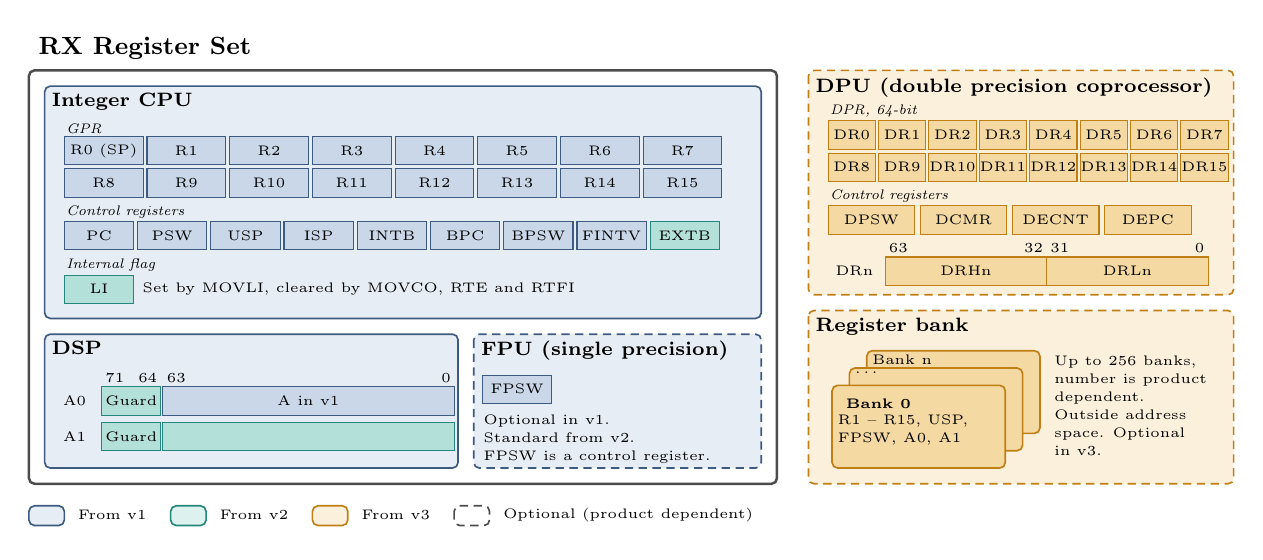
\begin{tikzpicture}[
  font=\scriptsize,
  box/.style={rounded corners=2pt, line width=0.6pt},
  c1/.style={box, fill=vonefill, draw=voneline},
  c2/.style={box, fill=vtwofill, draw=vtwoline},
  c3/.style={box, fill=vthrfill, draw=vthrline},
  cell/.style={draw, line width=0.4pt, minimum height=0.36cm, inner sep=0pt, font=\fontsize{5}{5}\selectfont},
  k1/.style={cell, fill=vonetile, draw=voneline},
  k2/.style={cell, fill=vtwotile, draw=vtwoline},
  k3/.style={cell, fill=vthrtile, draw=vthrline},
  opt/.style={dash pattern=on 3pt off 2pt},
  ttl/.style={font=\scriptsize\bfseries, anchor=north west, inner sep=1pt},
  sub/.style={font=\fontsize{5.5}{5.5}\selectfont\itshape, anchor=south west, inner sep=0.5pt},
  note/.style={font=\fontsize{5.5}{6.5}\selectfont, align=left, anchor=north west, inner sep=0.5pt},
  bit/.style={font=\fontsize{4.5}{4.5}\selectfont, anchor=south, inner sep=1pt}
]
% ======================= RX CPU =======================
\draw[box, draw=black!70, line width=0.9pt, fill=white] (0,0) rectangle (9.5,-5.25);
\node[font=\small\bfseries, anchor=south west] at (0,0.02) {RX Register Set};

% ---- Integer CPU ----
\draw[c1] (0.2,-0.2) rectangle (9.3,-3.15);
\node[ttl] at (0.25,-0.25) {Integer CPU};
\node[sub] at (0.45,-0.82) {GPR};
\foreach \i in {0,...,7} {
  \node[k1, minimum width=1.0cm] at ({0.95+\i*1.05},-1.02) {\ifnum\i=0 R0 (SP)\else R\i\fi};
  \pgfmathtruncatemacro{\j}{\i+8}
  \node[k1, minimum width=1.0cm] at ({0.95+\i*1.05},-1.43) {R\j};
}
\node[sub] at (0.45,-1.9) {Control registers};
\foreach \r [count=\i from 0] in {PC,PSW,USP,ISP,INTB,BPC,BPSW,FINTV} {
  \node[k1, minimum width=0.88cm] at ({0.89+\i*0.93},-2.1) {\r};
}
\node[k2, minimum width=0.88cm] at ({0.89+8*0.93},-2.1) {EXTB};
\node[sub] at (0.45,-2.58) {Internal flag};
\node[k2, minimum width=0.88cm] at (0.89,-2.78) {LI};
\node[note, anchor=west] at (1.42,-2.78) {Set by MOVLI, cleared by MOVCO, RTE and RTFI};

% ---- DSP ----
\draw[c1] (0.2,-3.35) rectangle (5.45,-5.05);
\node[ttl] at (0.25,-3.4) {DSP};
\node[bit, anchor=south west] at (0.93,-4.01) {71};
\node[bit, anchor=south east] at (1.67,-4.01) {64};
\node[bit, anchor=south west] at (1.71,-4.01) {63};
\node[bit, anchor=south east] at (5.40,-4.01) {0};
\foreach \a/\y in {A0/-4.2, A1/-4.65} {
  \node[font=\fontsize{5.5}{5.5}\selectfont, anchor=east] at (0.85,\y) {\a};
}
\node[k2, minimum width=0.75cm] at (1.3,-4.2) {Guard};
\node[k1, minimum width=3.7cm] at (3.55,-4.2) {A in v1};
\node[k2, minimum width=0.75cm] at (1.3,-4.65) {Guard};
\node[k2, minimum width=3.7cm] at (3.55,-4.65) {};

% ---- FPU ----
\draw[c1, opt] (5.65,-3.35) rectangle (9.3,-5.05);
\node[ttl] at (5.7,-3.4) {FPU (single precision)};
\node[k1, minimum width=0.88cm] at (6.2,-4.05) {FPSW};
\node[note] at (5.75,-4.35) {Optional in v1.\\Standard from v2.\\FPSW is a control register.};

% ======================= DPU (v3, optional) =======================
\draw[c3, opt] (9.9,0) rectangle (15.3,-2.85);
\node[ttl] at (9.95,-0.05) {DPU (double precision coprocessor)};
\node[sub] at (10.15,-0.62) {DPR, 64-bit};
\foreach \i in {0,...,7} {
  \pgfmathtruncatemacro{\j}{\i+8}
  \node[k3, minimum width=0.6cm, font=\fontsize{4.5}{4.5}\selectfont] at ({10.45+\i*0.64},-0.82) {DR\i};
  \node[k3, minimum width=0.6cm, font=\fontsize{4.5}{4.5}\selectfont] at ({10.45+\i*0.64},-1.23) {DR\j};
}
\node[sub] at (10.15,-1.7) {Control registers};
\foreach \r [count=\i from 0] in {DPSW,DCMR,DECNT,DEPC} {
  \node[k3, minimum width=1.1cm] at ({10.7+\i*1.17},-1.9) {\r};
}
\node[bit, anchor=south west] at (10.88,-2.36) {63};
\node[bit, anchor=south east] at (12.92,-2.36) {32};
\node[bit, anchor=south west] at (12.93,-2.36) {31};
\node[bit, anchor=south east] at (14.97,-2.36) {0};
\node[font=\fontsize{5.5}{5.5}\selectfont, anchor=west] at (10.12,-2.55) {DRn};
\node[k3, minimum width=2.05cm] at (11.9,-2.55) {DRHn};
\node[k3, minimum width=2.05cm] at (13.95,-2.55) {DRLn};

% ======================= Register bank (v3, optional) =======================
\draw[c3, opt] (9.9,-3.05) rectangle (15.3,-5.25);
\node[ttl] at (9.95,-3.1) {Register bank};
\foreach \d/\t in {0.44/Bank n, 0.22/\ldots} {
  \draw[box, fill=vthrtile, draw=vthrline] ({10.2+\d},{-4.0+\d}) rectangle ({12.4+\d},{-5.05+\d});
  \node[font=\fontsize{4.5}{4.5}\selectfont, anchor=north west, inner sep=1pt] at ({10.2+\d+0.03},{-4.0+\d-0.01}) {\t};
}
\draw[box, fill=vthrtile, draw=vthrline] (10.2,-4.0) rectangle (12.4,-5.05);
\node[font=\fontsize{5}{5}\selectfont\bfseries, anchor=north west] at (10.25,-4.05) {Bank 0};
\node[note] at (10.25,-4.35) {R1 -- R15, USP,\\FPSW, A0, A1};
\node[note] at (13.0,-3.6) {Up to 256 banks,\\number is product\\dependent.\\Outside address\\space. Optional\\in v3.};

% ======================= Legend =======================
\begin{scope}[shift={(0,-5.65)}]
\foreach \s/\t/\x in {c1/From v1/0, c2/From v2/1.8, c3/From v3/3.6} {
  \draw[\s] (\x,0.12) rectangle ++(0.45,-0.25);
  \node[font=\tiny, anchor=west] at (\x+0.5,0) {\t};
}
\draw[box, draw=black!70, opt] (5.4,0.12) rectangle ++(0.45,-0.25);
\node[font=\tiny, anchor=west] at (5.9,0) {Optional (product dependent)};
\end{scope}
\end{tikzpicture}
\captionsetup{font=scriptsize, labelfont=scriptsize}
\caption{RX register set. Color gives the version that introduced the element and dashed border marks 
an optional element. A0 extends v1 accumulator A with 8 guard bits, and A1 is added in v2.}
\figlabel{CArch.Summary.ISA.RX.RegisterSet}
\end{subfigure}

\vspace{0.5cm}

\begin{subfigure}{\linewidth}
\centering
\begin{tikzpicture}[
  tile/.style={draw, line width=0.4pt, minimum width=1.18cm, minimum height=0.33cm, inner sep=0pt,
               font=\fontsize{4.6}{4.6}\selectfont},
  t1/.style={tile, fill=vonetile, draw=voneline},
  t2/.style={tile, fill=vtwotile, draw=vtwoline},
  t3/.style={tile, fill=vthrtile, draw=vthrline},
  hd/.style={font=\fontsize{5.5}{5.5}\selectfont\itshape, inner sep=0.5pt},
  vl/.style={font=\scriptsize\bfseries, inner sep=1pt},
  optb/.style={draw=black!75, line width=0.7pt, dash pattern=on 2.5pt off 1.5pt},
  r1/.style={fill=vonefill}, r2/.style={fill=vtwofill}, r3/.style={fill=vthrfill}
]
\fill[r3, rounded corners=3pt] (-0.15,0.15) rectangle (16.670,-8.390);
\fill[r2, rounded corners=3pt] (-0.075,0.075) rectangle (13.800,-8.315);
\fill[r1, rounded corners=3pt] (0,0) rectangle (10.930,-8.240);
\node[vl, text=voneline, anchor=north east] at (10.880,-0.03) {RXv1};
\node[vl, text=vtwoline, anchor=north east] at (13.750,0.05) {RXv2};
\node[vl, text=vthrline, anchor=north east] at (16.620,0.13) {RXv3};
\node[hd, anchor=south west] at (0.250,-0.570) {Data Processing};
\node[t1] at (0.840,-0.785) {ABS};
\node[t1] at (2.080,-0.785) {ADC};
\node[t1] at (3.320,-0.785) {ADD};
\node[t1] at (0.840,-1.175) {CMP};
\node[t1] at (2.080,-1.175) {DIV};
\node[t1] at (3.320,-1.175) {DIVU};
\node[t1] at (0.840,-1.565) {EMUL};
\node[t1] at (2.080,-1.565) {EMULU};
\node[t1] at (3.320,-1.565) {MAX};
\node[t1] at (0.840,-1.955) {MIN};
\node[t1] at (2.080,-1.955) {MUL};
\node[t1] at (3.320,-1.955) {NEG};
\node[t1] at (0.840,-2.345) {SAT};
\node[t1] at (2.080,-2.345) {SATR};
\node[t1] at (3.320,-2.345) {SBB};
\node[t1] at (0.840,-2.735) {SUB};
\node[t1] at (2.080,-2.735) {TST};
\node[t1] at (0.840,-3.320) {AND};
\node[t1] at (2.080,-3.320) {NOT};
\node[t1] at (3.320,-3.320) {OR};
\node[t1] at (0.840,-3.710) {XOR};
\node[t1] at (0.840,-4.295) {REVL};
\node[t1] at (2.080,-4.295) {REVW};
\node[t1] at (3.320,-4.295) {ROLC};
\node[t1] at (0.840,-4.685) {RORC};
\node[t1] at (2.080,-4.685) {ROTL};
\node[t1] at (3.320,-4.685) {ROTR};
\node[t1] at (0.840,-5.075) {SHAR};
\node[t1] at (2.080,-5.075) {SHLL};
\node[t1] at (3.320,-5.075) {SHLR};
\node[hd, anchor=south west] at (4.160,-0.570) {Data Movement};
\node[t1] at (4.750,-0.785) {MOV};
\node[t1] at (5.990,-0.785) {MOVU};
\node[t1] at (4.750,-1.370) {POP};
\node[t1] at (5.990,-1.370) {POPC};
\node[t1] at (4.750,-1.760) {POPM};
\node[t1] at (5.990,-1.760) {PUSH};
\node[t1] at (4.750,-2.150) {PUSHC};
\node[t1] at (5.990,-2.150) {PUSHM};
\node[t1] at (4.750,-2.735) {SCCnd};
\node[t1] at (5.990,-2.735) {STNZ};
\node[t1] at (4.750,-3.125) {STZ};
\node[t1] at (5.990,-3.125) {XCHG};
\node[hd, anchor=south west] at (6.830,-0.570) {System};
\node[t1] at (7.420,-0.785) {MVTIPL};
\node[t1] at (8.660,-0.785) {RTE};
\node[t1] at (7.420,-1.175) {RTFI};
\node[t1] at (8.660,-1.175) {WAIT};
\node[t1] at (7.420,-1.760) {BRK};
\node[t1] at (8.660,-1.760) {CLRPSW};
\node[t1] at (7.420,-2.150) {INT};
\node[t1] at (8.660,-2.150) {MVFC};
\node[t1] at (7.420,-2.540) {MVTC};
\node[t1] at (8.660,-2.540) {NOP};
\node[t1] at (7.420,-2.930) {SETPSW};
\node[hd, anchor=south west] at (9.500,-0.570) {Control};
\node[t1] at (10.090,-0.785) {JMP};
\node[t1] at (10.090,-1.175) {JSR};
\node[t1] at (10.090,-1.760) {BCnd};
\node[t1] at (10.090,-2.150) {BRA};
\node[t1] at (10.090,-2.540) {BSR};
\node[t1] at (10.090,-3.125) {RTS};
\node[t1] at (10.090,-3.515) {RTSD};
\node[hd, anchor=south west] at (0.250,-5.660) {Array};
\node[t1] at (0.840,-5.875) {RMPA};
\node[t1] at (2.080,-5.875) {SSTR};
\node[t1] at (0.840,-6.265) {SUNTIL};
\node[t1] at (2.080,-6.265) {SWHILE};
\node[t1] at (0.840,-6.850) {SCMPU};
\node[t1] at (2.080,-6.850) {SMOVB};
\node[t1] at (0.840,-7.240) {SMOVF};
\node[t1] at (2.080,-7.240) {SMOVU};
\node[hd, anchor=south west] at (2.920,-5.660) {Bit};
\node[t1] at (3.510,-5.875) {BCLR};
\node[t1] at (3.510,-6.265) {BNOT};
\node[t1] at (3.510,-6.655) {BSET};
\node[t1] at (3.510,-7.045) {BTST};
\node[t1] at (3.510,-7.630) {BMCnd};
\node[hd, anchor=south west] at (4.350,-5.660) {DSP};
\node[t1] at (4.940,-5.875) {MACHI};
\node[t1] at (6.180,-5.875) {MACLO};
\node[t1] at (4.940,-6.265) {MULHI};
\node[t1] at (6.180,-6.265) {MULLO};
\node[t1] at (4.940,-6.850) {MVFACHI};
\node[t1] at (6.180,-6.850) {MVFACMI};
\node[t1] at (4.940,-7.240) {MVTACHI};
\node[t1] at (6.180,-7.240) {MVTACLO};
\node[t1] at (4.940,-7.825) {RACW};
\node[hd, anchor=south west] at (7.020,-5.660) {FPU};
\node[t1] at (7.610,-5.875) {FADD};
\node[t1] at (8.850,-5.875) {FCMP};
\node[t1] at (7.610,-6.265) {FDIV};
\node[t1] at (8.850,-6.265) {FMUL};
\node[t1] at (7.610,-6.655) {FSUB};
\node[t1] at (7.610,-7.240) {FTOI};
\node[t1] at (8.850,-7.240) {ITOF};
\node[t1] at (7.610,-7.630) {ROUND};
\draw[optb] (6.970,-5.360) rectangle (9.480,-7.835);
\node[hd, anchor=south west] at (11.130,-0.570) {DSP};
\node[t2] at (11.720,-0.785) {EMACA};
\node[t2] at (12.960,-0.785) {EMSBA};
\node[t2] at (11.720,-1.175) {EMULA};
\node[t2] at (12.960,-1.175) {MACLH};
\node[t2] at (11.720,-1.565) {MSBHI};
\node[t2] at (12.960,-1.565) {MSBLH};
\node[t2] at (11.720,-1.955) {MSBLO};
\node[t2] at (12.960,-1.955) {MULLH};
\node[t2] at (11.720,-2.540) {MVFACGU};
\node[t2] at (12.960,-2.540) {MVFACLO};
\node[t2] at (11.720,-2.930) {MVTACGU};
\node[t2] at (11.720,-3.515) {RACL};
\node[t2] at (12.960,-3.515) {RDACL};
\node[t2] at (11.720,-3.905) {RDACW};
\node[hd, anchor=south west] at (11.130,-4.440) {Data Movement};
\node[t2] at (11.720,-4.655) {MOVCO};
\node[t2] at (12.960,-4.655) {MOVLI};
\node[hd, anchor=south west] at (11.130,-5.190) {FPU};
\node[t2] at (11.720,-5.405) {FSQRT};
\node[t2] at (11.720,-5.990) {FTOU};
\node[t2] at (12.960,-5.990) {UTOF};
\node[hd, anchor=south west] at (14.000,-0.570) {DPU};
\node[t3] at (14.590,-0.785) {DABS};
\node[t3] at (15.830,-0.785) {DADD};
\node[t3] at (14.590,-1.175) {DCMPEQ};
\node[t3] at (15.830,-1.175) {DCMPLE};
\node[t3] at (14.590,-1.565) {DCMPLT};
\node[t3] at (15.830,-1.565) {DCMPUN};
\node[t3] at (14.590,-1.955) {DDIV};
\node[t3] at (15.830,-1.955) {DMUL};
\node[t3] at (14.590,-2.345) {DNEG};
\node[t3] at (15.830,-2.345) {DSQRT};
\node[t3] at (14.590,-2.735) {DSUB};
\node[t3] at (14.590,-3.320) {DROUND};
\node[t3] at (15.830,-3.320) {DTOF};
\node[t3] at (14.590,-3.710) {DTOI};
\node[t3] at (15.830,-3.710) {DTOU};
\node[t3] at (14.590,-4.100) {FTOD};
\node[t3] at (15.830,-4.100) {ITOD};
\node[t3] at (14.590,-4.490) {UTOD};
\node[t3] at (14.590,-5.075) {DMOV};
\node[t3] at (15.830,-5.075) {DPOPM};
\node[t3] at (14.590,-5.465) {DPUSHM};
\node[t3] at (15.830,-5.465) {MVFDC};
\node[t3] at (14.590,-5.855) {MVFDR};
\node[t3] at (15.830,-5.855) {MVTDC};
\draw[optb] (13.950,-0.270) rectangle (16.460,-6.060);
\node[hd, anchor=south west] at (14.000,-6.490) {Bit};
\node[t3] at (14.590,-6.705) {BFMOV};
\node[t3] at (15.830,-6.705) {BFMOVZ};
\node[hd, anchor=south west] at (14.000,-7.340) {Register Bank};
\node[t3] at (14.590,-7.555) {RSTR};
\node[t3] at (15.830,-7.555) {SAVE};
\draw[optb] (13.950,-7.040) rectangle (16.460,-7.760);
\draw[-{Latex[length=4pt]}, line width=0.8pt, draw=voneline] (-0.15,-8.690) -- (10.930,-8.690) node[pos=0.5, fill=white, inner sep=1.5pt, font=\tiny\bfseries, text=voneline] {RXv1};
\draw[-{Latex[length=4pt]}, line width=0.8pt, draw=vtwoline] (-0.15,-9.070) -- (13.800,-9.070) node[pos=0.5, fill=white, inner sep=1.5pt, font=\tiny\bfseries, text=vtwoline] {RXv2};
\draw[-{Latex[length=4pt]}, line width=0.8pt, draw=vthrline] (-0.15,-9.450) -- (16.670,-9.450) node[pos=0.5, fill=white, inner sep=1.5pt, font=\tiny\bfseries, text=vthrline] {RXv3};
\end{tikzpicture}
\captionsetup{font=scriptsize, labelfont=scriptsize}
\caption{Summary of Opcodes in RX ISA by version. Each version includes all instructions of the previous version. 
Instructions are clustered on the basis of Nature of operation performed and within nature split into bands 
separated by a gap, in alphabetical order. Dashed border marks optional instructions -- FPU in v1 (Standard 
from v2), DPU and Register Bank instructions in v3.}
\figlabel{CArch.Summary.ISA.RX.ISet.OpcodeSummary}
\end{subfigure}

\captionsetup{font=scriptsize, labelfont=scriptsize}
\caption{RX Register Set and Opcodes at glance for v1, v2 and v3}
\figlabel{CArch.Summary.ISA.RX.RFile.ISet.OpcodeSummary}
\end{figure}


\SOPNoteLabel{CArch.Summary.ISA.RX.Note.2}
\SOPNoteHead{2. Register Set}
\SOPNoteBody

(1) \emph{Data Registers:} %
\figref{CArch.Summary.ISA.RX.RegisterSet} shows the register set of the RX CPU. RX has following data registers:

    \leveltwo
    (a) \emph{GPR:} %
    Sixteen 32-bit General Purpose Registers (R0 -- R15), with R0 acting as stack pointer. SP is 
    assembler alias to R0.

    (b) \emph{DPR:} %
    Sixteen 64-bit Double Precision Registers (DR0 -- DR15), when double precision coprocessor is present.
    Higher and Lower 32 bits of DPR can be accessed separately with data movement instructions using 
    DRH0 -- DRH15 and DRL0 -- DRL15.

    (c) \emph{A:} %
    One 64-bit accumulator in v1 implied by instruction syntax, and two addressable 72-bit accumulators 
    (A0 and A1) in v2 and v3.

\levelone
(2) \emph{Control Registers:} %
RX has following control registers:

    \leveltwo
    (a) \emph{Program Counter (PC):} %
    Program counter holds address of instruction being executed. At reset, PC is loaded from reset 
    vector at 0xFFFFFFFC.

    (b) \emph{Interrupt and User Stack Pointer (ISP, USP):} %
    ISP and USP hold interrupt and user stack pointer values. Contents of current stack pointer (R0/SP)
    map to ISP or USP depending on value of PSW.U bit.

    (c) \emph{Fast Interrupt handling (FINTV, BPC and BPSW):} %
    When a fast interrupt happens, contents of PC and PSW are saved in Backup Program Counter (BPC) 
    and Backup PSW (BPSW) and PC is set to contents of Fast Interrupt Vector (FINTV). This enables 
    fast response time for fast interrupt.

    (d) \emph{Vector table (INTB, EXTB):} %
    INTB holds base address of interrupt vector table. EXTB (v2 and v3) holds base address of 
    exception vector table and is set to 0xFFFFFF80 at reset. Vector tables are covered in 
    \SOPNoteRef{CArch.Summary.ISA.RX.Note.13}{Section 13(2)}.

    (e) \emph{Status Word (PSW, FPSW and DPSW) and DP Control Registers:} %
    Status word registers hold the results of instructions executed and the state of CPU. 
    Processor Status Word (PSW) is present in all RX processors. PSW is detailed in 
    \SOPNoteRef{CArch.Summary.ISA.RX.Note.3}{Section 3(5)}.
    
    RX Processors with single and double precision floating point support have Floating 
    Point Status Word (FPSW) and Double Precision Floating Point Status Word (DPSW) registers
    respectively. In addition to DPSW, DPU has three more control registers -- DCMR, DECNT and
    DEPC. These registers are detailed in \SOPNoteRef{CArch.Summary.ISA.RX.Note.11}{Section 11}.

\levelone
(3) \emph{Register Bank:} %
Exception handlers save the registers they use on entry and restore them on exit, normally using 
the stack. For faster save and restore, v3 provides register banks (numbered 0 to 255). These 
register banks are outside the address space and can be accessed only through privileged 
instructions SAVE and RSTR.

Availability of register banks and number of register banks are \emph{implementation defined}.

SAVE instruction saves registers R1 -- R15, USP, FPSW, A0 and A1 to the specified register bank. 
RSTR instruction restores registers R1 -- R15, USP, FPSW, A0 and A1. R0 (SP), PC and PSW are not 
saved. R0 is the active stack pointer, and PC and PSW are saved on the stack (or in BPC/BPSW for 
fast interrupt) on exception acceptance.

(4) \emph{LI:} %
v2 and v3 have a 1-bit LI flag internal to the CPU, used for exclusive access to memory -- 
linked load and conditional store. MOVLI, MOVCO, RTE and RTFI are the only instructions that 
access LI.




\SOPNoteLabel{CArch.Summary.ISA.RX.Note.3}
\SOPNoteHead{3. RX CPU Overview}
\SOPNoteBody

(1) \emph{Address Space and Data Size Terms:} %
RX is a 32-bit CPU with byte addressing. With 32-bit byte address, address space for RX CPU is 
4 GB with address in range 0x00000000 -- 0xFFFFFFFF.

Terms byte, word, longword and double longword correspond to 8, 16, 32 and 64-bit data types.

(2) \emph{ISA Versions:} %
RX CPU has three versions of ISA with a separate ISA reference manual for each of them. They are referred to as 
v1 (\cite{rx_v1_um}), v2 (\cite{rx_v2_um}) and v3 (\cite{rx_v3_um}) in this document. ISA reference manuals for v2 
and v3 also have a section in which additions made to previous version are noted. 
\figref{CArch.Summary.ISA.RX.RFile.ISet.OpcodeSummary} shows Register Set and Opcodes across three ISA versions. 
v1 $\subset$ v2 $\subset$ v3, so backward compatibility is maintained. 

    \leveltwo
    (a) \emph{v1:} %
    In v1, FPU (Floating Point Unit) is an optional component. DSP module has one accumulator that is 
    64 bits wide.

    (b) \emph{v2:} %
    In v2, FPU is made a standard component. Support is added for square root (FSQRT) and conversion 
    from/to unsigned integer (UTOF, FTOU). Non-destructive (three operand Rs, Rs2, Rd) versions 
    of floating point addition, subtraction and multiplication instructions are introduced. In DSP module, 
    number of accumulators is raised to 2 (A0 and A1) and width of accumulator is increased to 72 bits. 
    Fourteen new DSP instructions are added and accumulator contents can be shifted before reading. 
    In Integer CPU, STZ and STNZ can have register source operand. Exclusive access to memory is 
    added with MOVLI, MOVCO and LI flag, which is also cleared by RTE and RTFI. EXTB control register is
    introduced allowing for relocatable exception vector table.

    (c) \emph{v3:} %
    In v3, DPU (Double Precision Unit) coprocessor is introduced as an optional component. Two new 
    bit manipulation instructions supporting bit range movement are introduced. Register bank 
    facilitating faster context save and restore is introduced as an optional component with the 
    number of banks being product dependent. Non-destructive (three operand) version of XOR instruction 
    is introduced.

\levelone
In instruction reference tables, by default instructions are available from v1, unless opcode 
is marked with superscript 2 (available from v2) or 3 (available from v3). Table caption states 
version when it applies to all instructions in the table.

(3) \emph{Classification: Group, Nature, Type and Category:} %
Group and Nature are two different approaches to cluster instructions, each with its own benefit.
Type and Category are used for second level of clustering within a cluster based on Nature.

    \leveltwo
    (a) \emph{Group:} %
    Group is a set of instructions that share instruction encoding space in which only bits that vary 
    between them are those identifying the opcode ($C_x$). Each instruction encoding belongs to 
    exactly one group. Instructions in a group share the same operand fields.
    
    Clustering of instructions into groups enables compact instruction encoding diagrams and 
    simplifies the implementation of instruction decoder.

    (b) \emph{Nature and Type:} %
    Instead of presenting instructions in alphabetical order, instructions are clustered based on nature
    of operation performed. Type sub-clusters instructions within a cluster. Nature and Type form a 
    two-level taxonomy for instructions, which enables quicker understanding and easier recall.

    Instruction reference tables are organized by Nature. Type column in these tables is used to identify 
    the sub-cluster within the cluster.

    (c) \emph{Category:} %
    Category sub-clusters instructions within a Nature based on cycles taken. Cycles count tables 
    (\tabref{CArch.Summary.ISA.RX.Cycles}) are organized by Nature and Category.

\levelone
(4) \emph{Instruction Encoding:} %
RX instruction encoding uses a variable length instruction format, with length of the instruction 
ranging from 1 to 8 bytes. According to \cite{rxv3_details}, as shorter encodings are assigned to 
more frequently used instructions, this encoding reduces static and dynamic code size compared to 
a RISC CPU with Load-Store architecture.

RX instruction encoding has two parts -- standard and extension bytes. Standard bytes hold fields 
from which presence and length of extension bytes can be determined. Extension bytes are used for 
storing immediate and displacement values. Refer to 
\SOPNoteRef{CArch.Summary.ISA.RX.Note.7}{Section 7(4)} for more details on extension bytes.

(5) \emph{Processor Status Word:} %
The fields of PSW are:

    \leveltwo
    (a) \emph{Flags (C, Z, S and O):} %
    Four LSB bits represent four flags. They are C - Carry, Z - Zero, S - Sign and O - Overflow.

    (b) \emph{Interrupt Enable (I):} %
    When set, interrupts are enabled. 

    (c) \emph{Stack Pointer Select Bit (U):} %
    U = 1 $\implies$ stack pointer is USP and U = 0 $\implies$ stack pointer is ISP.

    (d) \emph{Processor Mode Select Bit (PM):} %
    PM = 0 $\implies$ processor is in supervisor mode and PM = 1 $\implies$ processor is in user
    mode.

    (e) \emph{Processor Interrupt Priority Level (IPL):} %
    Possible values are 0 (lowest) to 15 (highest). When an interrupt is taken, its priority 
    level is recorded in IPL. As interrupts with priority level less than or equal to IPL 
    are not processed, a handler is not preempted by an interrupt of equal or lower priority.

\begin{figure}
\begin{center}
\scriptsize
\begin{tabular}{cccccccccccccccc}
b31 & b30 & b29 & b28 & b27 & b26 & b25 & b24 & b23 & b22 & b21 & b20 & b19 & b18 & b17 & b16 \\ \hline
\multicolumn{1}{|c}{-} &
\multicolumn{1}{|c}{-} &
\multicolumn{1}{|c}{-} &
\multicolumn{1}{|c}{-} &
\multicolumn{4}{|c}{IPL[3:0]} & 
\multicolumn{1}{|c}{-} &
\multicolumn{1}{|c}{-} &
\multicolumn{1}{|c}{-} &
\multicolumn{1}{|c}{PM} & 
\multicolumn{1}{|c}{-} &
\multicolumn{1}{|c}{-} &
\multicolumn{1}{|c}{U} &
\multicolumn{1}{|c|}{I} \\ \hline
&&&&&&&&&&&&&&& \\ 
b15 & b14 & b13 & b12 & b11 & b10 & b9 & b8 & b7 & b6 & b5 & b4 & b3 & b2 & b1 & b0 \\ \hline
\multicolumn{1}{|c}{-} &
\multicolumn{1}{|c}{-} &
\multicolumn{1}{|c}{-} &
\multicolumn{1}{|c}{-} &
\multicolumn{1}{|c}{-} &
\multicolumn{1}{|c}{-} &
\multicolumn{1}{|c}{-} &
\multicolumn{1}{|c}{-} &
\multicolumn{1}{|c}{-} &
\multicolumn{1}{|c}{-} &
\multicolumn{1}{|c}{-} &
\multicolumn{1}{|c}{-} &
\multicolumn{1}{|c}{O} &
\multicolumn{1}{|c}{S} &
\multicolumn{1}{|c}{Z} &
\multicolumn{1}{|c|}{C} \\ \hline
\end{tabular}
\end{center}
\captionsetup{font=scriptsize, labelfont=scriptsize}
\caption{Processor Status Word. Value is 0 after reset.}
\figlabel{CArch.Summary.ISA.RX.CtrlReg.PSW}
\end{figure}

\levelone
(6) \emph{Processor Mode:} %
RX processor has two modes -- User and Supervisor. At reset, processor is in supervisor mode. Current 
mode is indicated by PSW.PM bit. Access control restrictions and mode switching are provided below:

    \leveltwo
    (a) \emph{Privileged Instructions:} %
    Privileged instructions are instructions that can be executed only when CPU is in supervisor 
    mode. Execution of privileged instructions in user mode generates privileged instruction 
    exception. Privileged instructions are RTE, RTFI, WAIT, MVTIPL, SAVE and RSTR.

    (b) \emph{Restriction in write access:} %
    In user mode, write to following control registers -- ISP, INTB, EXTB, BPC, BPSW and FINTV and 
    I, U, PM and IPL fields of PSW are ignored. In supervisor mode, write to PSW.PM is ignored.

    (c) \emph{Switching Processor Modes:} %
    When an exception is generated and accepted, PSW.PM is set to 0 and CPU switches to supervisor mode.
    Returning from exception/fast interrupt using RTE or RTFI with restored PSW.PM having value of 1 
    causes processor to switch to user mode.


\levelone
(7) \emph{Accumulator:} %
With respect to accumulator in DSP module of RX

    \leveltwo
    (a) \emph{Count:} %
    v1 has one accumulator; v2/v3 have two, A0 and A1.

    (b) \emph{Width:} %
    16-bit MUL/MAC type instructions write A[63:16] in v1 and Ax[71:16] in v2/v3. MUL clears the 
    lower 16 bits and MAC/MSB leave them unchanged. So, effective width is 48 of 64 bits in v1. 
    In v2/v3, 32-bit MUL/MAC instructions also use the lower 16 bits, so all 72 bits are used.

    (c) \emph{Headroom:} %
    Above the product, headroom is 16 bits in v1 and 24 bits in v2/v3 for 16-bit signed inputs, 
    and 8 bits in v2/v3 for 32-bit signed inputs.

    (d) \emph{As scratch:} %
    Accumulator (in v1) and A0 (in v2/v3) are used as a scratch register by following multiply related 
    instructions -- MUL, EMUL, EMULU, FMUL and RMPA. So, if contents of the accumulator are needed, 
    they need to be preserved before using these instructions.

\levelone    
(8) \emph{Array Operations:} %
RX provides instructions that operate on one or two arrays of input data. Operands are implicit
with R1 holding address, R2 holding address/value and R3 holding the maximum iteration count.
RMPA instruction also uses R6:R5:R4, which hold the sum. These instructions are interruptible 
and the number of cycles these instructions take for execution depends on number of iterations 
and size of data type.




\SOPNoteLabel{CArch.Summary.ISA.RX.Note.4}
\SOPNoteHead{4. Notations}
\SOPNoteBody

\levelone
(1) \emph{Mapping Tables:} %
Following tables provide mapping information

    \leveltwo
    (a) \tabref{CArch.Summary.ISA.RX.IEncode.Code.Opcode.Mapping} provides mapping between Code field 
    used in machine code and opcode used in assembly code for all instruction groups. 

    (b) \tabref{CArch.Summary.ISA.RX.IEncode.Immediate.Mapping} provides mapping between imm value 
    used in machine code and immediate values used in assembly code.

    (c) \tabref{CArch.Summary.ISA.RX.IEncode.Operand.Mapping} provides mapping between bit fields 
    used in machine code and operands used in assembly code.

\levelone    
(2) \emph{Register File Fields:} %
Fields in relation to data and control registers are:

    \leveltwo
    (a) \emph{General Purpose Register:} %
    Rd, Rd2, Rs, Rs2, Rb and Ri are used to identify general purpose registers R0 -- R15. Rd and 
    Rd2 correspond to destination register. Rs and Rs2 correspond to source register. Rb and Ri 
    correspond to base and index registers.

    They are 4-bit fields, except in LD.SOFF.S, LD.SOFF.U, ST.SOFF and DM.IMS, where 3-bit fields 
    represent R0 -- R7.

    In syntax, X-X2 (e.g. Rs-Rs2, DRd-DRd2) denotes the range of registers from X to X2.

    (b) \emph{Double Precision Register:} %
    DRs, DRs2, DRd and DRd2 are 4-bit fields identifying 64-bit DPU registers; DRHx and DRLx identify 
    their higher and lower 32 bits. s denotes source and d destination.

    (c) \emph{Accumulator:} %
    A is a 1-bit field used to identify A0 and A1 in v2 and v3 based processors. A-bit is set to 0 in 
    instruction encoding for v1 as it has only one accumulator.

    (d) \emph{Double Precision Control Register:} %
    DCRs, DCRs2, DCRd and DCRd2 are 4-bit fields used to identify double precision control registers. 
    
    (e) \emph{Control Register:} %
    Cr is a 4-bit field identifying a control register. 1101 (EXTB) is reserved in v1. 

    (f) \emph{PSW flags:} %
    flag is a 4-bit field used to identify 1-bit flag fields in PSW. It is used by CLRPSW and SETPSW
    instructions to clear/set flags. 

\levelone    
(3) \emph{Opcode Fields:} %
Fields in relation to opcode are:

    \leveltwo
    (a) \emph{Code ($C_x$):} %
    Code is the concatenation of $C_x$ fields and identifies the opcode of the instruction.

    (b) \emph{Condition Code (cd):} %
    cd is a 4-bit field used to represent condition. It is used in conditional branch (B$<$Cond$>$) and 
    conditional movement instructions (SC$<$Cond$>$ and BM$<$Cond$>$). 

    (c) \emph{Size (sz):} %
    sz is a 1 or 2-bit field used to represent size of data type in the operation performed. 

\levelone    
(4) \emph{Operand Fields:} %
Fields in relation to operand are:

    \leveltwo
    (a) \emph{Length of immediate (li):} %
    For many instruction groups with an immediate operand, immediate value is added as suffix. li 
    represents the length of immediate value in the suffix. When length of immediate value is less 
    than 32 bits, it is sign extended to 32 bits.

    (b) \emph{Length of displacement (ld, ldd, lds):} %
    For many instruction groups with memory operand, optional displacement (offset) value is added as 
    suffix. ld represents the length of displacement value in suffix, if it exists. It is also used 
    to identify addressing mode used for operand -- Register Direct, Register Indirect and Register
    Relative with 8 or 16-bit unsigned scaled displacement. 
    
    Scale value depends on size of operand except for double precision, for which it is scaled by 
    4 bytes. See \SOPNoteRef{CArch.Summary.ISA.RX.Note.14}{Section 14(1)} for more details on scale 
    factor for double precision.

    ldd and lds correspond to ld value of destination and source memory operands for data movement 
    from memory to memory.

    (c) \emph{Memory Information (mi) and Memory Extension (me):} %
    Data type of memory operand is identified based on sz or mi field. When these fields are not 
    present in encoding for instruction group, it is UB (Unsigned Byte).

    mi field is used to identify data type of memory operand as one of the following -- 8-bit 
    Signed Byte (B), 16-bit Signed Word (W), 16-bit Unsigned Word (UW) and 32-bit Long (L).

    me field is used in instruction reference and corresponds to memory extension, giving data 
    type of memory operand -- UB when encoding has no mi field, otherwise B, W, L or UW given 
    by mi.

    (d) \emph{Sequential addressing (ad):} %
    RX supports sequential load and store operations in which address register is updated with 
    next or previous location along with load/store operation. Supported addressing modes are 
    post-increment and pre-decrement. ad is used to identify operation (load/store) and addressing
    mode for sequential memory operations.

    (e) \emph{Number of registers (nm):} %
    Instruction encoding for double precision stack operations uses starting register index and 
    number of registers to identify a sequential set of registers. nm represents number of 
    registers - 1.

\levelone    
(5) \emph{Immediate Fields:} %
imm corresponds to concatenated $I_x$ fields. Symbols used in instruction reference are grouped 
below; encoding and value ranges are in \tabref{CArch.Summary.ISA.RX.IEncode.Immediate.Mapping}.

    \leveltwo
    (a) \emph{Shift count:} %
    sh1 (DSP.RND), sh2 (DSP.FAC, 0 in v1) and sh (shift and rotate).

    (b) \emph{Bit position:} %
    bp3 (bit in a byte in memory), bp5 (bit in a register), and s, d, w (BFMOV and BFMOVZ source LSB, 
    destination LSB and width).

    (c) \emph{Unsigned value:} %
    ipl (MVTIPL). uimm4 and uimm8, zero-extended to 32 bits. suimm8 is scaled by 4 (RTSD frame size).

    (d) \emph{Displacement:} %
    dsp5 and dsp, scaled by operand size as noted in (4)(b). sdsp and ddsp are source and destination 
    displacements of memory to memory transfer.

    (e) \emph{Long immediate:} %
    limm is 8, 16, 24 or 32 bits, with length given by li and sign extended as noted in (4)(a). imm32 is 
    used by FPU and DPU instructions.

\levelone
(6) \emph{PC Relative Offset Fields:} %
pcdsp3, pcdsp8, pcdsp16 and pcdsp24 hold the branch offset from PC. pcdsp8/\allowbreak 16/\allowbreak 24 
are signed and pcdsp3 encodes offsets 3 to 10, as listed in \tabref{CArch.Summary.ISA.RX.IEncode.Immediate.Mapping}.



\SOPNoteLabel{CArch.Summary.ISA.RX.Note.5}
\SOPNoteHead{5. Addressing Modes}
\SOPNoteBody

Addressing modes specify how operand is obtained. Addressing modes available in RX are

(1) \emph{Register Direct:} %
Operand is contents of register.

    \leveltwo
    (a) R0 -- R15: Operand is contents of GPR.

    (b) DR0 -- DR15: Operand is contents of 64-bit DPR.

    (c) DRL0 -- DRL15: Operand is lower 32 bits of 64-bit DPR.

    (d) DRH0 -- DRH15: Operand is upper 32 bits of 64-bit DPR.

    (e) A0, A1: Operand is contents of Accumulator.

\levelone
(2) \emph{Control Register:} %
Operand is contents of control register.

    \leveltwo
    (a) Cr: Operand is contents of CPU control register including FPSW.

    (b) DCR: Operand is contents of DPU control register.

\levelone
Possible values for Cr and DCR are given in \tabref{CArch.Summary.ISA.RX.IEncode.Operand.Mapping}.

(3) \emph{PSW Flags (flag):} %
Operand is 1-bit flag in PSW register. Possible values for flag field are given in 
\tabref{CArch.Summary.ISA.RX.IEncode.Operand.Mapping}.

(4) \emph{Register Indirect ([Rn]):} %
Effective address is Rn.

(5) \emph{Register Relative (dsp[Rn]):} %
Effective address is Rn + dsp.

(6) \emph{Indexed Register Indirect ([Ri, Rb]):} %
Effective address is Rb + Ri * Sizeof(sz).

(7) \emph{Post-Increment ([Rn+]):} %
Effective address is Rn and Rn = Rn + Sizeof(sz).

(8) \emph{Pre-Decrement ([-Rn]):} %
Effective address is Rn - Sizeof(sz). Rn = Rn - Sizeof(sz).

(9) \emph{Immediate:} %
Immediate operands are constant values coded along with the instruction. List of immediate 
operands is outlined in \SOPNoteRef{CArch.Summary.ISA.RX.Note.4}{Section 4(5)} and how they
are encoded is available in \tabref{CArch.Summary.ISA.RX.IEncode.Immediate.Mapping}.

(10) \emph{PC Relative:} %
Branch target address is PC + pcdsp for BRA, BSR and B$<$Cond$>$, and PC + Rs for BRA.L and BSR.L. 
pcdsp fields are given in \SOPNoteRef{CArch.Summary.ISA.RX.Note.4}{Section 4(6)}.



\SOPNoteLabel{CArch.Summary.ISA.RX.Note.6}
\SOPNoteHead{6. Instruction Set Reference}
\SOPNoteBody

(1) \emph{Nature and Type:} %
RX instructions are clustered and sub-clustered into Nature and Type to facilitate quick recall. Each Nature has 
a separate table and Type information is in the first column.

    \leveltwo
    (a) Integer ALU: Arithmetic Instructions -- \tabref{CArch.Summary.ISA.RX.IRef.IALU.Arithmetic}, Bitwise and 
    Shift Instructions -- \tabref{CArch.Summary.ISA.RX.IRef.IALU.Bitwise}.

    (b) Bit Manipulation Instructions -- \tabref{CArch.Summary.ISA.RX.IRef.BitManipulation}.

    (c) Data Movement Instructions -- \tabref{CArch.Summary.ISA.RX.IRef.DataMove}.

    (d) Control Transfer Instructions -- \tabref{CArch.Summary.ISA.RX.IRef.Control}.

    (e) System Instructions -- \tabref{CArch.Summary.ISA.RX.IRef.System}.

    (f) DSP Instructions -- \tabref{CArch.Summary.ISA.RX.IRef.DSP}.

    (g) Array Instructions -- \tabref{CArch.Summary.ISA.RX.IRef.Array}.

    (h) FPU Instructions -- \tabref{CArch.Summary.ISA.RX.IRef.FPU}.

    (i) DPU Instructions -- \tabref{CArch.Summary.ISA.RX.IRef.DPU}.

\levelone
(2) \emph{Flag Updates:} %
Instruction reference tables carry a flags column that shows whether and how an instruction updates 
Overflow (O), Sign (S), Zero (Z) and Carry (C) flags of PSW using the codes below:

    \leveltwo
    (a) \emph{Standard (*):} %
    Flags are updated by standard rule.

    (b) \emph{Unchanged (-):} %
    Flags are not updated.

    (c) \emph{Custom (!):} %
    Flags are updated as shown in Operation column.

\levelone
Standard rules are as follows:

    \leveltwo
    (a) \emph{O (Overflow):} %
    O is set to 1 when the result of arithmetic operation overflows, with 32-bit inputs considered 
    as signed integers. It is set to 0, otherwise.

    (b) \emph{S (Sign):} %
    MSB of the result. Typically, S = Rd[31].

    (c) \emph{Z (Zero):} %
    Z = (result == 0). Typically, Z = (Rd == 0). For FPU, both +0 and -0 set Z.

    (d) \emph{C (Carry):} %
    Based on operation:

        \levelthree
        (i) For addition, C is set to 1 when the result overflows, with inputs considered as 
        unsigned integers.

        (ii) For subtraction, C is set to 1 when no borrow occurs, i.e. Rs2/Rd $\ge$ Rs as unsigned
        integers.

        (iii) For shift, C is the last bit shifted out and is set to 0 when shift count is 0.

        (iv) For ROTL and ROTR, C = LSB and MSB of result respectively.

\levelone
(3) \emph{Group:} %
Group column lists all encoding groups used by instructions in the block. Groups differ either
because opcodes in the block are in different groups, or because the same instruction is encoded
in different groups based on operand (e.g. AB.LD1 for register direct and UB, AB.MI1 for other
memex). Group of each opcode is given in \tabref{CArch.Summary.ISA.RX.IEncode.Code.Opcode.Mapping}.

(4) \emph{Table format:} %
Instruction reference tables have three levels. A Type has one or more blocks. A block is a
combination of Group and Syntax, and a change in either starts a new block. A block has one or
more instructions, each given by Opcode and Operation. Type, Group and Syntax are shown on the
first row of the block and are blank for the remaining rows. Text that does not fit in a cell
continues on the next row.

$<$opc$>$ in Syntax stands for the opcode in the Opcode column.

\levelone
(5) \emph{Operation:} %
The Operation column in instruction reference tables uses the following conventions:

    \leveltwo
    (a) \emph{Bit fields:} %
    x[n] is bit n of x. x[m:n] is bits m down to n of x. a:b is concatenation of a and b with 
    a in upper bits. 

    (b) \emph{Functions:} %
    Functions used are:

        \levelthree
        (i) Convert(x, src, dst [, rm]): Converts value x of type src to type dst using rounding 
        mode rm. src, dst $\in$ \{S32, U32, F32, F64\} -- 32-bit signed integer, 32-bit unsigned
        integer, single and double precision. rm is RZ (round towards zero), FPSW.RM or DPSW.DRM.
        rm is omitted when conversion is exact, which happens when dst is F64.

        (ii) IsNaN(x): 1 when floating point value x is NaN (not a number, quiet or signalling), 
        otherwise 0.

        (iii) Mem(addr, type): addr is byte address of memory location. type $\in$ \{B, UB, W, 
        UW, L, D\}. On read, B and W are sign extended and UB and UW are zero extended to 
        32 bits. D is 64-bit double precision value. On write, lower 8, 16, 32 or 64 bits are 
        stored based on the type.

        (iv) MemSeq(addr, type, n): n consecutive memory locations of Sizeof(type) bytes 
        starting at addr. Assigning \{Ra, ..., Rb\} to it (or it to \{Ra, ..., Rb\}) stores 
        (loads) registers Ra to Rb with Ra at lowest address. n is Rb - Ra + 1.

        (v) Saturate(x, n): Saturates x to n-bit signed data range.

        (vi) SignExtend(x), ZeroExtend(x): Sign or zero extends x to width of destination.

        (vii) Sizeof(type): Number of bytes for the type -- 1 for B/UB, 2 for W/UW, 4 for L and
        8 for D.

    \leveltwo
    (c) \emph{Shift operators:} %
    x $\lsl$ n and x $\lsr$ n are logical left and right shifts of x by n bits. x $\asr$ n is 
    arithmetic right shift. Shift by 32 or more bits gives 0 for $\lsl$ and $\lsr$ and sign 
    bits of x for $\asr$.

    (d) \emph{Signedness:} %
    Integer arithmetic and comparison operators are signed. Operators with subscript u ($*_u$, 
    $/_u$, $\ge_u$) treat their operands as unsigned.

    (e) \emph{Operators:} %
    Operators and statements (if, while) follow C language (?:, $\mid\mid$, \&\&, ==, \&, $\mid$, 
    $\sim$, $++$, $--$, $+=$ and $-=$), with $\ne$, $\le$ and $\ge$ for !=, $<$= and $>$=. $\oplus$ is 
    bitwise XOR.

    (f) \emph{Condition:} %
    Cond Pass is true when condition specified by $<$Cond$>$ is satisfied based on flags in PSW
    as noted in \tabref{CArch.Summary.ISA.RX.IEncode.Operand.Mapping}.

    (g) \emph{Temporaries:} %
    t, t1 and t2 hold intermediate values.



\SOPNoteLabel{CArch.Summary.ISA.RX.Note.7}
\SOPNoteHead{7. Instruction Encoding}
\SOPNoteBody

(1) \emph{Encoding diagrams and tables:} %
Instruction encoding maps machine code to assembly code. To decode, start at 
\figref{CArch.Summary.ISA.RX.IEncoding.EntryPoint} and follow the gray shaded fields to the instruction group; Opcode 
(\tabref{CArch.Summary.ISA.RX.IEncode.Code.Opcode.Mapping}) and Operand 
(\tabref{CArch.Summary.ISA.RX.IEncode.Operand.Immediate.Mapping}) tables then give the opcode and operands when read
along with instruction reference tables. To encode, start from the Group column of the instruction reference.

The encoding diagrams and tables were verified by a disassembler implemented from them alone, which disassembles 
assembled test code covering all instruction variants.

(2) \emph{Field restrictions:} %
Fields described in Section 4 can take any value, except for restrictions noted in 
\tabref{CArch.Summary.ISA.RX.IEncode.Field.Restrictions}.

\begin{table}
\begin{center}
\scriptsize
\setlength{\tabcolsep}{4pt}
\begin{tabular}{lll}
\hline
Field            & Constraint                                       & Applies to                                        \\ \hline
A                & In v1, A = 0                                     & All                                               \\
                 &                                                  &                                                   \\
ad               & ad[1] = 1                                        & Load (LD.SEQ.S, LD.SEQ.U)                         \\
                 & ad[1] = 0                                        & Store (ST.SEQ)                                    \\
                 &                                                  &                                                   \\
cd               & cd $\ne$ 1111                                    & All                                               \\
                 & cd $\ne$ 1110                                    & All, except CTL.IMM.B                             \\
                 &                                                  &                                                   \\
Cr               & In v1, Cr $\ne$ EXTB                             & All                                               \\
                 & Cr $\ne$ PC                                      & Cr is destination (POPC, MVTC)                    \\
                 &                                                  &                                                   \\
ld               & ld = 11                                          & AB.LD2 (ABS, ADC, NEG, NOT, SBB)                  \\
                 & lds, ldd $\ne$ 11                                & DM.MM                                             \\
                 & ld $\ne$ 11                                      & AB.MI1(C), AB.MI2(C), BM.IM1(C), BM.IM2, BM.IM3   \\
                 & ld $\ne$ 11                                      & DM.IM, DM.XCHG.MI, LD.OFF.S, ST.OFF               \\
                 & ld $\ne$ 11                                      & FPU.I2F.MI, STK.SIM, DPU.LD, DPU.ST               \\
                 & ld = 11 $\implies$ sz = 10                       & DM.CRES                                           \\
                 &                                                  &                                                   \\
li               & li = 01 (.B), li $\in$ \{01, 10\} (.W)           & DM.IM                                             \\
                 &                                                  &                                                   \\
mi               & mi = 10                                          & AB.MI2 (ADC, SBB)                                 \\
                 &                                                  &                                                   \\
nm               & DRs/DRd + nm $\le$ 15                            & DPU.PUSH, DPU.POP                                 \\
                 & DCRs/DCRd + nm $\le$ 3                           & DPU.PUSHC, DPU.POPC                               \\
                 &                                                  &                                                   \\
Rd-Rd2           & Rd, Rd2 $\ne$ 0; Rd $\le$ Rd2                    & CTL.ACR (RTSD)                                    \\
                 &                                                  &                                                   \\
Rd-Rd2, Rs-Rs2   & First $\ne$ 0; First $<$ Last                    & STK.MI (PUSHM), STK.MO (POPM)                     \\
                 &                                                  &                                                   \\
sh2              & In v1, sh2 = 0. In v2/v3, sh2 $\in$ \{0, 1, 2\}  & All                                               \\
                 &                                                  &                                                   \\
sz               & sz $\ne$ 11                                      & When 2 bits wide                                  \\ \hline
\end{tabular}
\end{center}
\captionsetup{font=scriptsize, labelfont=scriptsize}
\caption{Restrictions on instruction encoding fields. Reserved values of Cr, DCR and flag are shown as - in 
\tabref{CArch.Summary.ISA.RX.IEncode.Operand.Mapping}. Suffix (C) on a group denotes the group and its C 
variant (e.g. AB.MI1(C) is AB.MI1 and AB.MI1C). For AB.LD2 and AB.MI2, restrictions apply only to 
instructions in brackets.}
\tablabel{CArch.Summary.ISA.RX.IEncode.Field.Restrictions}
\end{table}

\levelone
(3) \emph{Composite Immediate:} %
imm field holds multiple operands in the following instruction groups:

    \leveltwo
    (a) DM.IMS: uimm8 = $I_0$ and dsp5 = $I_2:I_1$.

    \leveltwo
    (b) BM.RNG: d = imm[9:5]; s = (d - imm[4:0]) \& 31; w = (imm[14:10] - d) \& 31 and imm[15] = 0.

\levelone
(4) \emph{Standard and Extension bytes:} %
Standard bytes hold the fixed fields of an instruction. Extension bytes hold displacement and immediate values whose 
lengths are given by li, ld, ldd and lds; they are not shown in the encoding diagrams. Extension bytes follow the 
standard bytes in the following order:

    \leveltwo
    (a) \emph{li only:} %
    An 8, 16, 24 or 32-bit immediate, as given by li.

    (b) \emph{ld only:} %
    An 8 or 16-bit displacement, as given by ld. Exception: In DPU.LD and DPU.ST, extension bytes come between B2 
    and B3 (carrying DRd/DRs).

    (c) \emph{ld and li (DM.IM):} %
    Displacement, followed by immediate.

    (d) \emph{lds and ldd (DM.MM):} %
    Source displacement, followed by destination displacement.

\levelone
Diagrams show only B0--B3. FPU.IMM, DPU.RTLI and DPU.RTHI have 7 standard bytes, with a 32-bit immediate in the 
last four. BM.RNG has 5, with a 16-bit immediate in the last two. These partially shown immediates are marked 
$I_0'$.


\begin{figure}
\centering
\newcommand{\partonep}{5}
\newcommand{\partthreep}{4}
\newcommand{\parttwop}{3}
\newcommand{\parttwoap}{2}
\newcommand{\partfourp}{1}
\newcommand{\partfourap}{0}

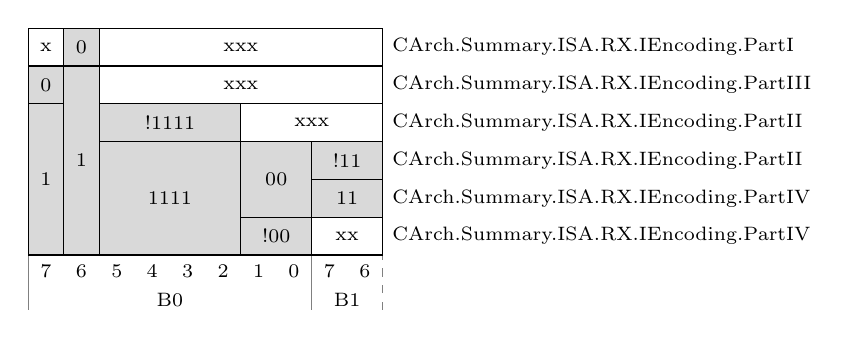
\begin{tikzpicture}[xscale=0.45,yscale=0.24]
\foreach \x in {0, 1, ..., 9}
    \draw (\x + 0.5, 1) node[anchor=north] {\scriptsize \pgfmathparse{int(7 - mod(\x, 8))}\pgfmathresult};
\draw (4, -0.5) node[anchor=north] {\scriptsize B0};
\draw (9, -0.5) node[anchor=north] {\scriptsize B1};
\foreach \x in {0, 8}
    \draw[gray] (\x, -1.9) -- (\x, 1);
\draw[gray, dashed] (10, -1.9) -- (10, 1);
% Instruction decode path
% B1(7)
\fill[black!15] (0, \partthreep * 2 + 1) rectangle (1, \partthreep * 2 + 3);
\fill[black!15] (0, \partfourap * 2 + 1) rectangle (1, \parttwop * 2 + 3);
% B1(6)
\fill[black!15] (1, \partonep * 2 + 1) rectangle (2, \partonep * 2 + 3);
\fill[black!15] (1, \partfourap * 2 + 1) rectangle (2, \partthreep * 2 + 3);
% B1(5)
\fill[black!15] (2, \parttwop * 2 + 1) rectangle (6, \parttwop * 2 + 3);
\fill[black!15] (2, \partfourap * 2 + 1) rectangle (6, \parttwoap * 2 + 3);
% B1(1)
\fill[black!15] (6, \partfourp * 2 + 1) rectangle (8, \parttwoap * 2 + 3);
\fill[black!15] (6, \partfourap * 2 + 1) rectangle (8, \partfourap * 2 + 3);
% B2(7)
\fill[black!15] (8, \parttwoap * 2 + 1) rectangle (10, \parttwoap * 2 + 3);
\fill[black!15] (8, \partfourp * 2 + 1) rectangle (10, \partfourp * 2 + 3);

% Encoding
% B1(7)
\draw (0, \partonep * 2 + 1) rectangle (1, \partonep * 2 + 3) node[pos=.5] {\scriptsize x};
\draw (0, \partthreep * 2 + 1) rectangle (1, \partthreep * 2 + 3) node[pos=.5] {\scriptsize 0};
\draw (0, \partfourap * 2 + 1) rectangle (1, \parttwop * 2 + 3) node[pos=.5] {\scriptsize 1};
% B1(6)
\draw (1, \partonep * 2 + 1) rectangle (2, \partonep * 2 + 3) node[pos=.5] {\scriptsize 0};
\draw (1, \partfourap * 2 + 1) rectangle (2, \partthreep * 2 + 3) node[pos=.5] {\scriptsize 1};
% B1(5)
\draw (2, \partonep * 2 + 1) rectangle (10, \partonep * 2 + 3) node[pos=.5] {\scriptsize xxx};
\draw (2, \partthreep * 2 + 1) rectangle (10, \partthreep * 2 + 3) node[pos=.5] {\scriptsize xxx};
\draw (2, \parttwop * 2 + 1) rectangle (6, \parttwop * 2 + 3) node[pos=.5] {\scriptsize !1111};
\draw (2, \partfourap * 2 + 1) rectangle (6, \parttwoap * 2 + 3) node[pos=.5] {\scriptsize 1111};
% B1(1)
\draw (6, \parttwop * 2 + 1) rectangle (10, \parttwop * 2 + 3) node[pos=.5] {\scriptsize xxx};
\draw (6, \partfourp * 2 + 1) rectangle (8, \parttwoap * 2 + 3) node[pos=.5] {\scriptsize 00};
\draw (6, \partfourap * 2 + 1) rectangle (8, \partfourap * 2 + 3) node[pos=.5] {\scriptsize !00};
% B2(7)
\draw (8, \parttwoap * 2 + 1) rectangle (10, \parttwoap * 2 + 3) node[pos=.5] {\scriptsize !11};
\draw (8, \partfourp * 2 + 1) rectangle (10, \partfourp * 2 + 3) node[pos=.5] {\scriptsize 11};
\draw (8, \partfourap * 2 + 1) rectangle (10, \partfourap * 2 + 3) node[pos=.5] {\scriptsize xx};

% Group names
\draw (10, \partonep * 2 + 2) node[anchor=west] {\scriptsize \figref{CArch.Summary.ISA.RX.IEncoding.PartI}};
\draw (10, \partthreep * 2 + 2) node[anchor=west] {\scriptsize \figref{CArch.Summary.ISA.RX.IEncoding.PartIII}};
\draw (10, \parttwop * 2 + 2) node[anchor=west] {\scriptsize \figref{CArch.Summary.ISA.RX.IEncoding.PartII}};
\draw (10, \parttwoap * 2 + 2) node[anchor=west] {\scriptsize \figref{CArch.Summary.ISA.RX.IEncoding.PartII}};
\draw (10, \partfourp * 2 + 2) node[anchor=west] {\scriptsize \figref{CArch.Summary.ISA.RX.IEncoding.PartIV}};
\draw (10, \partfourap * 2 + 2) node[anchor=west] {\scriptsize \figref{CArch.Summary.ISA.RX.IEncoding.PartIV}};
\end{tikzpicture}
\captionsetup{font=scriptsize, labelfont=scriptsize}
\caption{RX Instruction Encoding Entry Point.}
\figlabel{CArch.Summary.ISA.RX.IEncoding.EntryPoint}
\end{figure}



\SOPNoteLabel{CArch.Summary.ISA.RX.Note.8}
\SOPNoteHead{8. Cycles Count}
\SOPNoteBody

(1) \emph{Sources:} %
Information presented in this section is based on the pipeline and number of cycles sections in the CPU chapter 
of Group User Manuals for

    \leveltwo
    (a) v1: From RX100 Series: RX110 (\cite{rx_110}), RX111 (\cite{rx_111}), RX113 (\cite{rx_113}), 
    RX130 (\cite{rx_130}) and RX13T (\cite{rx_13T}).

    \leveltwo
    (b) v2: From 
    
        \levelthree
        (i) RX100 Series: RX140 (\cite{rx_140}) and RX14T (\cite{rx_14T}).
        
        (ii) RX200 Series: RX230 and RX231 (\cite{rx_230}), RX23E-A (\cite{rx_23ea}), RX23E-B (\cite{rx_23eb}), 
        RX23T (\cite{rx_23t}), RX23W (\cite{rx_23w}), RX24T (\cite{rx_24t}) and RX24U (\cite{rx_24u}).
    
        (iii) RX600 Series: RX65N and RX651 (\cite{rx_65n}).
        
        (iv) RX700 Series: RX71M (\cite{rx_71m}).

    \leveltwo
    (c) v3: From
    
        \levelthree
        (i) RX200 Series: RX260 and RX261 (\cite{rx_260}) and RX26T (\cite{rx_26t}).
        
        (ii) RX600 Series: RX660 (\cite{rx_660}), RX66N (\cite{rx_66n}), RX66T (\cite{rx_66t}) and 
        RX671 (\cite{rx_671}).

        (iii) RX700 Series: RX72M (\cite{rx_72m}), RX72N (\cite{rx_72n}) and RX72T (\cite{rx_72t}).

\levelone
These were the groups that were marked as active as of Oct-2026 on Renesas website. 
\tabref{CArch.Summary.ISA.RX.Cycles} provides instruction cycles with zero-wait access.
Cycles are the same in v1, v2 and v3, except for FADD, FSUB and FMUL instructions.

(2) \emph{Throughput and Latency:} %
Throughput is the number of cycles after which the next instruction can start. Latency is the 
number of cycles after which a following instruction can use the result. Latency helps to
determine the pipeline stall due to RAW (Read After Write) hazard when a subsequent 
instruction uses the result. 

(3) \emph{Guidelines to avoid pipeline stalls:} %
Methods for avoiding pipeline stalls are:

    \leveltwo
    (a) \emph{Load Stall:} %
    Instructions with throughput:latency cycles (Load, POP, POPC, POPM, MOVLI, RTSD with register 
    list, DMOV load and DPOPM) stall when the next instruction uses the last loaded register.
    Place an instruction without RAW dependency between them. 

    (b) \emph{DPU ALU Stall:} %
    DPU arithmetic, comparison and conversion instructions take 1 additional cycle if 
    subsequent instruction is DPU Movement or Sign injection instructions (DABS, DNEG) with
    RAW dependency. This stall can be avoided by ensuring that DPU ALU instruction is not 
    followed by DPU Movement/Sign injection instruction or DPU movement/sign injection 
    instruction doesn't use DPU ALU output.

    (c) \emph{Memory Source Operand Stall:} %
    An Integer or FPU ALU instruction with memory source operand is split into load and ALU 
    micro-operations. ALU operation waits for the load, which adds 2 cycles. With a spare register, 
    load into it, place an instruction without RAW dependency next and then operate on the register. 
    This fills the stall with useful work at the cost of one more instruction.

    (d) \emph{Memory to Memory Stall:} %
    MOV and PUSH with memory source take 3 cycles. Load into a spare register followed by store 
    or PUSH also takes 3 cycles, as store waits for the loaded data, but saves 1 cycle when 
    an instruction without RAW dependency is placed between them.

\levelone    
(4) \emph{Memory stalls:} %
Cycles in \tabref{CArch.Summary.ISA.RX.Cycles} are per instruction and do not include instruction 
fetch stalls, which add cycles to an instruction sequence. Similarly, memory access need not be 
zero-wait state and can introduce stalls. They are outside the scope of this document.

(5) \emph{Superscalar:} %
According to \cite{rx_brochure, rxv3_details, rx_ooo}, all RX processors use a five-stage pipeline with following 
stages -- IF (Instruction Fetch), D (Decode), E (Execute), M (Memory) and WB (Write Back).


    \leveltwo
    (a) v1 is a single-issue CPU.

    (b) v2 is superscalar, with separate execution paths for Integer/DSP operations, memory 
    access and FPU operations. 

    (c) v3 is also superscalar with improvements in combination of instructions that can be 
    executed together.

\levelone
Hence, cycles of an instruction sequence on v2 and v3 can be fewer than the sum of its 
instruction cycles. However, detailed pairing rules are not published by Renesas and 
are outside the scope of this document.



\SOPNoteLabel{CArch.Summary.ISA.RX.Note.9}
\SOPNoteHead{9. Intrinsics and Inline assembly}
\SOPNoteBody

(1) \emph{Intrinsics:} %
Intrinsic functions provide function call interface to instructions that have no straightforward
mapping in C language. This lets programmer hint to compiler on instruction to be used.
\tabref{CArch.Summary.ISA.RX.Intrinsics} provides list of intrinsics available in CC-RX. Points to note:

    \leveltwo
    (a) \emph{machine.h:} %
    CC-RX provides two versions of intrinsics. \tabref{CArch.Summary.ISA.RX.Intrinsics} shows version
    with \_\_ prefix, which is available from V2.05.00. The second version, without the prefix, is 
    available in all versions and requires machine.h to be included.

    (b) \emph{Trigonometric function unit:} %
    Certain RX processors have trigonometric function unit. CC-RX provides intrinsics to access them.
    They are outside the scope of this document at this time. See \cite{rx_compiler} for details on those intrinsics.

\levelone
(2) \emph{Inline assembly:} %
CC-RX provides \#pragma inline\_asm $<$func$>$, which has to be added before a function definition.
Such function's body can be filled with assembly instructions. Calling conventions noted in 
\SOPNoteRef{CArch.Summary.ISA.RX.Note.10}{Section 10} are applicable for these functions as well. 
Some points to note are:

    \leveltwo
    (a) \emph{static:} %
    Calls are always expanded inline, whenever possible. Defining the function as static removes 
    its definition after expansion; otherwise, an external definition is also generated.

    (b) \emph{Restrictions:} %
    Only RX instructions and temporary labels (?:, referenced by ?+ and ?-) are allowed. Other 
    labels, assembler directives and a final RTS are not allowed.



\SOPNoteLabel{CArch.Summary.ISA.RX.Note.10}
\SOPNoteHead{10. Calling Conventions}
\SOPNoteBody

(1) \emph{Scope limit:} %
For simplicity, we restrict scope of this section with following assumptions. For details of calling 
conventions without these restrictions, refer to CC-RX manual (\cite{rx_compiler}).

    \leveltwo
    (a) \emph{Fundamental data types:} %
    Only fundamental data types (1, 2, 4 and 8-byte signed/unsigned integers, single/double precision
    floating point and pointer) are passed as argument and provided as return value.

    (b) \emph{No vaarg:} %
    Functions called have fixed number of parameters.

    (c) \emph{Double Size:} %
    Code is compiled with dbl\_size = 8.

\levelone    
(2) \emph{Fundamental data types:} %
Sizes of fundamental data types and their alignment requirement are provided in 
\tabref{CArch.Summary.ISA.RX.DataTypes.Size.Align}.

\begin{table}
\begin{center}
\scriptsize
\begin{tabular}{lrr|lrr}
\hline
Data type & Size & Alignment & Data type & Size & Alignment \\ \hline
char      & 1    & 1         & float     & 4    & 4         \\
short     & 2    & 2         & double    & 8    & 4         \\
int       & 4    & 4         & long      & 4    & 4         \\
long long & 8    & 4         & pointer   & 4    & 4         \\ \hline
\end{tabular}
\end{center}
\captionsetup{font=scriptsize, labelfont=scriptsize}
\caption{Fundamental data types, their size and alignment in RX. char data type corresponds to unsigned char and 
signed\_char option makes it signed char. When int\_to\_short option is used, size 
and alignment of int data type is same as that of short. With dbl\_size = 4, double is treated as single precision 
floating point data type. 8-byte data types (long long and double) require only 4-byte alignment.}
\tablabel{CArch.Summary.ISA.RX.DataTypes.Size.Align}
\end{table}

\levelone
(3) \emph{Fixed Function Registers:} %
Following compiler options reserve general purpose registers for a fixed function. These registers cannot 
be used for any other purpose.

    \leveltwo
    (a) \emph{fint\_register:} %
    Reserves 0 to 4 registers for fast interrupt, allocated downward from R13 -- R13, R12 -- R13, 
    R11 -- R13 and R10 -- R13 for 1 to 4 registers.

    (b) \emph{pid:} %
    Reserves one register for position independent data access. It is the highest register not 
    reserved by fint\_register, i.e. R13, R12, R11, R10 and R9 for fint\_register 0 to 4. 
    nouse\_pid\_register keeps the same register unused, for code called from a PID-enabled 
    application.

    (c) \emph{base:} %
    Can be used for allocating any available registers in R8 -- R13 to any of the base areas 
    including ROM, RAM or any fixed address.

\levelone
Fixed Function registers are always from R8 -- R13, when defined.

(4) \emph{Scratch and Persistent Registers:} %
Registers are classified into scratch and persistent based on whether their contents can be modified by 
the callee without preservation (scratch) or with preservation (persistent).

    \leveltwo
    (a) \emph{Scratch:} %
    Callee may modify them; caller saves them if their contents are needed after the call. R1 -- R5, 
    R14, R15, PSW, FPSW, Accumulator (A/A0, A1), DPSW, DECNT and DEPC belong to this category.

    (b) \emph{Persistent:} %
    Callee saves and restores them if it uses them. R0, R6 -- R13, DR0 -- DR15 and DCMR belong to this 
    category.

\levelone
(5) \emph{Parameter Passing:} %
Parameters are allocated from left to right to registers R1--R4 or to parameter area in stack as noted
below:

    \leveltwo
    (a) \emph{Registers:} %
    Parameter is allocated to lowest numbered free register(s) as noted below:

        \levelthree
        (i) \emph{One register:} %
        Integer data types of length up to 4 bytes, float and pointer are passed using one register. 
        Signed and Unsigned integer data types of size smaller than 32 bits are sign and zero 
        extended and stored in the register.

        (ii) \emph{Two registers:} %
        long long and double take up eight bytes and require two registers. Lower 4 bytes are
        stored in lower numbered register.

    \leveltwo
    (b) \emph{Parameter Area in Stack:} %
    When no free registers are available or parameter needs more than available free registers, 
    they are placed in the stack with their address aligned in accordance with data type. 
    Parameters after them can still use free registers.

    (c) \emph{Stack frame:} %
    On function entry, SP points to Return PC and Parameter Area starts at SP + 4. It is caller's
    responsibility to set up stack frame before BSR/JSR instruction and clean it up on return from
    callee.

\levelone
(6) \emph{Return value:} %
For fundamental data type return value with size less than or equal to 4 bytes, R1 holds the 
return value. Integer data types of size less than 4 bytes are sign or zero extended to 32 bits 
based on their data type. 

For long long and double data types of length 8 bytes, R2:R1 holds the return value.



\SOPNoteLabel{CArch.Summary.ISA.RX.Note.11}
\SOPNoteHead{11. Floating Point}
\SOPNoteBody

(1) \emph{FPSW and DPSW:} %
Bit fields of FPSW and DPSW and their functions are identical, with D prefixed in DPSW as shown in 
\tabref{CArch.Summary.ISA.RX.FltPt.FPSW} and \tabref{CArch.Summary.ISA.RX.FltPt.DPSW}. We use 
FPSW names in this sub-section. Enabled FP exceptions generate an exception in FPU and 
an interrupt in DPU.

(2) \emph{Rounding mode (RM):} %
Two-bit RM field selects rounding applied when result is inexact

    \leveltwo
    (a) 00: Round to nearest with ties to even
    
    (b) 01: Round towards zero
    
    (c) 10: Round towards $+\infty$ 
    
    (d) 11: Round towards $-\infty$

\levelone
(3) \emph{Denormalized number handling (DN and CE):} %
RX FPU/DPU doesn't process IEEE 754 denormalized numbers in hardware. For FPU, programmer is provided 
with two options:

    \leveltwo
    (a) \emph{Flush to zero (DN = 1):} %
    When DN = 1, positive and negative denormalized numbers are treated as +0 and -0 respectively.
    Destination gets result with that treatment. This is a hardware-only solution for handling 
    denormalized numbers.

    (b) \emph{Software implementation through exception handler (DN = 0):} %
    When DN = 0, a denormalized input or underflowed result sets CE (Unimplemented processing) and
    raises an exception. CE has no enable bit and cannot be masked. Exception handler could generate
    the result in software.

    This option is valid for FPU, as exception is raised at faulting instruction and cannot be
    masked. For DPU, exception is reported as interrupt, which is accepted only when PSW.I and 
    PSW.IPL allow. Instructions executed before the interrupt is accepted cannot be undone. 
    So, software implementation is not possible for DPU.

\levelone    
(4) \emph{IEEE 754 Exceptions handling (X, U, Z, O and V):} %
IEEE 754 specifies five FP exceptions in a floating point operation -- Inexact (X), Underflow (U), 
Division by zero (Z), Overflow (O) and Invalid (V). For $j \in \{X, U, Z, O, V\}$, one of the 
options below is chosen separately for each exception:

    \leveltwo
    (a) \emph{Sticky flags ($E_j = 0$):} %
    FP Exception is masked by setting $E_j$ field to 0. Destination gets default result. $F_j$ is 
    a sticky flag and it records occurrence of these exceptions until cleared by software. FS is 
    exception error summary, obtained with logical OR of FU, FZ, FO and FV fields (FX is excluded).

    (b) \emph{Exception handler ($E_j = 1$):} %
    Exception is raised and destination is not updated. $F_j$ is not changed. Handler can read 
    $C_j$ to determine the cause.

\levelone    
(5) \emph{Cause Flags ($C_j$):} %
Every floating point instruction sets or clears cause flags, regardless of $E_j$. When needed, 
they must be read before execution of next floating point instruction. For DPU, this does not 
apply when first occurrence of exception information is preserved as noted in (6).

(6) \emph{Preserve FP Exception details for ISR in DPU (DECNT and DEPC):} %
DPU reports an enabled FP exception (DE$_j$) as an interrupt, so further double precision 
instructions may execute before the ISR runs (PSW.I, PSW.IPL). DECNT.EHM selects what the ISR sees:

    \leveltwo
    (a) \emph{Last Instruction (DECNT.EHM = 0):} %
    Cause flags reflect the last double precision instruction executed and DEPC the last one that 
    triggered an FP exception. So, unless only one exception is enabled, ISR cannot tell which 
    exception occurred or which instruction caused it first.

    (b) \emph{First Instruction (DECNT.EHM = 1):} %
    DEPC holds the address of the first faulting instruction and DECNT.EHS is set to 1. While 
    EHS = 1, DPSW and DEPC are not updated and further FP exception interrupts are held back. 
    ISR writes 0 to EHS to release the hold.

\levelone
(7) \emph{Comparison result (DCMR):} %
Comparison instructions write the result of comparison in DCMR.RES field. It is set to 0 when 
comparison is not passed and 1 when it is passed. Result can be transferred to PSW.Z using 
MVFDR instruction or read to GPR using MVFDC instruction.

(8) \emph{Alias:} %
DPSW, DCMR, DECNT and DEPC are also referred to as DCR0, DCR1, DCR2 and DCR3. This order defines
register range in DPUSHM.L and DPOPM.L (e.g. DPUSHM.L DCR0 -- DCR2 saves DPSW--DECNT).

\levelone
(9) \emph{NaN:} %
Signaling NaN (SNaN) and Quiet NaN (QNaN) are represented with MSB of the fraction being 0 and 
1 respectively. 



\SOPNoteLabel{CArch.Summary.ISA.RX.Note.12}
\SOPNoteHead{12. Pseudo Instructions}
\SOPNoteBody

\tabref{CArch.Summary.ISA.RX.PseudoInstructions} provides the list of pseudo instructions available in RX and the
mapping between assembly code written and assembled code. SUB with immediate beyond uimm4 is accepted by GNU 
assembler and assembled as ADD with negated immediate value. CC-RX doesn't accept it, so programmer has to 
use ADD with negated value.

\begin{table}
\scriptsize
\begin{center}
\begin{tabular}{ll|ll}
\hline
Assembly code         & Assembled Code         & Assembly code               & Assembled Code                  \\ \hline
ADD \#limm, Rd        & ADD \#limm, Rd, Rd     &                             &                                 \\
                      &                        &                             &                                 \\
BZ label              & BEQ label              & SCZ.L Rd/SCZ.sz dsp[Rd]     & SCEQ.L Rd/SCEQ.sz dsp[Rd]       \\
BNZ label             & BNE label              & SCNZ.L Rd/SCNZ.sz dsp[Rd]   & SCNE.L Rd/SCNE.sz dsp[Rd]       \\
BC label              & BGEU label             & SCC.L Rd/SCC.sz dsp[Rd]     & SCGEU.L Rd/SCGEU.sz dsp[Rd]     \\
BNC label             & BLTU label             & SCNC.L Rd/SCNC.sz dsp[Rd]   & SCLTU.L Rd/SCLTU.sz dsp[Rd]     \\
                      &                        &                             &                                 \\
BMZ \#bp5, Rd         & BMEQ \#bp5, Rd         & BMZ \#bp3, dsp[Rd].B        & BMEQ \#bp3, dsp[Rd].B           \\
BMNZ \#bp5, Rd        & BMNE \#bp5, Rd         & BMNZ \#bp3, dsp[Rd].B       & BMNE \#bp3, dsp[Rd].B           \\
BMC \#bp5, Rd         & BMGEU \#bp5, Rd        & BMC \#bp3, dsp[Rd].B        & BMGEU \#bp3, dsp[Rd].B          \\
BMNC \#bp5, Rd        & BMLTU \#bp5, Rd        & BMNC \#bp3, dsp[Rd].B       & BMLTU \#bp3, dsp[Rd].B          \\ \hline
\end{tabular}
\end{center}
\captionsetup{font=scriptsize, labelfont=scriptsize}
\caption{Pseudo Instructions in RX. Conditions \{Z, NZ, C, NC\} map to \{EQ, NE, GEU, LTU\}.}
\tablabel{CArch.Summary.ISA.RX.PseudoInstructions}
\end{table}


\SOPNoteLabel{CArch.Summary.ISA.RX.Note.13}
\SOPNoteHead{13. Exceptions}
\SOPNoteBody

Exception is an event that requires stopping the regular flow of execution and starting another. 
Interrupts are one kind of exception. In this section, basic information on exceptions is
provided. Interested readers can refer to ISA manuals 
(\cite{rx_v1_um, rx_v2_um, rx_v3_um}) for more details.

(1) \emph{List of exceptions:} %
Exceptions in RX are: 

    \leveltwo
    (a) \emph{Undefined Instruction Exception:} %
    This exception is raised when an instruction encoding that doesn't belong to ISA is executed.

    (b) \emph{Privileged Instruction Exception:} %
    Raised when a privileged instruction (\SOPNoteRef{CArch.Summary.ISA.RX.Note.3}{Section 3(6)(a)}) 
    is executed in user mode.

    (c) \emph{Access Exception:} %
    When memory protection unit detects access errors, this exception is raised.

    (d) \emph{Address Exception:} %
    When 64-bit memory operand is accessed with an address that is not multiple of 4, this 
    exception is raised. This exception is applicable only to v3 as such access can only be
    done with DPU.

    (e) \emph{Single Precision Floating Point Exception:} %
    This exception is raised when a single precision floating point operation causes an IEEE 754 
    exception (overflow, underflow, inexact, division-by-zero or invalid operation) whose enable 
    bit $E_j$ in FPSW is 1, or an unimplemented processing exception, which is raised when FPSW.DN = 0 
    and an input or result is a denormalized number.

    (f) \emph{Reset:} %
    When reset signal is provided to CPU, reset handler takes over. Reset brings the 
    processor to a known state. Unlike other exceptions noted above, execution starts afresh
    in case of reset.

    (g) \emph{Non-Maskable Interrupt:} %
    When an interrupt signal which cannot be masked with PSW.I = 0 arrives, this exception
    is raised.

    (h) \emph{Interrupt:} %
    When the CPU receives an interrupt signal, control is transferred to interrupt handler 
    when PSW.I = 1 and priority level of the interrupt is higher than PSW.IPL. Fast interrupt 
    saves PC and PSW in BPC and BPSW instead of stack.

    (i) \emph{Unconditional trap:} %
    This occurs through BRK or INT instruction.

\levelone
(2) \emph{Vector Table:} %
Exception vector table has 32 entries of 4-byte handler address (128 bytes). Entry index for 
privileged instruction, access, undefined instruction, address, single precision floating point 
and non-maskable interrupt are 20, 21, 23, 24, 25 and 30 respectively. Reset handler address is 
always at 0xFFFFFFFC. In v1, the table is fixed at 0xFFFFFF80. In v2 and v3, its base address is 
in EXTB.

Interrupt vector table has 256 entries of 4-byte handler address (1024 bytes), with base address 
in INTB. BRK uses entry 0 and INT takes entry index as its argument. For fast interrupt, handler 
address is taken from FINTV instead.

(3) \emph{Interrupts and Floating Point Exceptions:} %
Interrupts are asynchronous -- raised by signals through the interrupt controller, maskable by PSW.I 
and IPL, and taken between instructions. Other exceptions are synchronous -- raised by the instruction 
itself, not maskable, with saved PC pointing to that instruction.

Floating point exception refers to an IEEE 754 condition (or unimplemented processing) detected by a 
floating point operation. It is always flagged in FPSW/DPSW and raises a processor event only when 
enabled ($E_j = 1$), or always in case of unimplemented processing (when FPSW.DN/DPSW.DDN = 0). 
For single precision, the event is the exception in (1)(e) -- synchronous, with saved PC pointing 
to the floating point instruction. For double precision, DPU sends an interrupt request to the 
interrupt controller -- asynchronous, maskable, and taken after the CPU may have executed further 
instructions. So, DEPC records the PC of the floating point instruction and DECNT preserves the 
first occurrence until the handler releases it when DECNT.EHM = 1.



\SOPNoteLabel{CArch.Summary.ISA.RX.Note.14}
\SOPNoteHead{14. Deviations from manuals}
\SOPNoteBody

Instruction reference, encoding and cycles tables were cross-checked against the ISA manuals 
(\cite{rx_v1_um, rx_v2_um, rx_v3_um}) and group manuals listed in \SOPNoteRef{CArch.Summary.ISA.RX.Note.8}{Section 
8(1)}. Ambiguous cases were resolved by assembling test code with CC-RX. Deviations found are listed below:

(1) \emph{DMOV.D:} %
For DMOV.D in register relative addressing mode, scale factor for displacement is 4 in Section 3 and 8 
in Section 4 of \cite{rx_v3_um}. So, one of them is wrong. We tried following

    \leveltwo
    (a) Assembled with offset of $2^{16} * 4$, which should work if scale factor is 8. CC-RX gave 
    ``Value is out of range''. 

    (b) Assembled with offset of 4, which should be rejected if scale factor is 8. CC-RX accepted it.

\levelone
So, scale factor is 4.

(2) \emph{CMP Encoding:} %
In Section 4 for CMP instruction with register or memory operand, in instruction encoding Rd is shown 
in place of Rs2. CMP instruction doesn't have destination register.

(3) \emph{FSQRT with immediate operand:} %
Section 3 of v2 (\cite{rx_v2_um}) lists FSQRT \#IMM:32, Rd. It has no encoding in Section 4 and is not 
present in v3. Assembling FSQRT with immediate operand gave an error. So, FSQRT doesn't support immediate 
operand.



\SOPNoteLabel{CArch.Summary.ISA.RX.Note.15}
\SOPNoteHead{15. Future and Related Work}
\SOPNoteBody

(1) \emph{Complementary Materials:} %
Following are complementary materials to this guide.

    \leveltwo
    (a) \emph{Slides and Video:} %
    This guide is written as a quick reference for professional programmers who are already familiar 
    with RX ISA. For those familiar with other Instruction sets like AArch32 or RISC-V, review the 
    YT Video that provides an overview of RX CPU and how various concepts are arranged in the QRG before
    diving into this QRG.

    (b) \emph{Quiz, Lab Programs and Performance Engineering Problem Set:} %
    Quiz questions to test understanding of concepts are arranged based on section. Lab Programs 
    are designed to check understanding of various assembly language programming constructs.

    Performance Engineering Problem Set is designed to check programmer's ability to do:
    
        \levelthree
        (i) \emph{Optimization:} %
        Perform architecture specific optimization
        
        (ii) \emph{Estimation:} %
        Estimate instruction count and CPU cycles of algorithm/implementation alternatives and 
        arrive at optimal implementation without implementing them, within the scope noted in 
        Section 1 and with (2)(b) for v2/v3.
        
        (iii) \emph{Verification:} %
        Implement the optimal variation and verify that estimated cycles match with actual 
        cycles.

\levelone
Recommended flow is:

    Watch YT Video $\Rightarrow$ Read QRG and Solve Quiz Questions $\Rightarrow$ Write Lab Programs
    $\Rightarrow$ Solve Performance Engineering Problem Set.

\levelone
(2) \emph{Related Work:} %
Work that makes use of information provided in this QRG includes ISA Projects, Pipeline and Memory 
characterization.

    \leveltwo
    (a) \emph{ISA Projects:} %
    Following ISA projects can be implemented based on Instruction set reference tables and 
    Instruction encoding available in \SOPNoteRef{CArch.Summary.ISA.RX.Note.6}{Section 6}
    and \SOPNoteRef{CArch.Summary.ISA.RX.Note.7}{Section 7}.

        \levelthree
        (i) \emph{Tools:} %
        Tool based projects such as assembler, disassembler and instruction set simulator can
        be created.

        (ii) \emph{IST:} %
        Instruction Set Test Code, which provides function call interface to all instruction
        variants can be used to verify understanding of instructions.

    \leveltwo
    (b) \emph{CPU Pipeline Characterization:} %
    While instruction cycles are available in the manuals and summarized in
    \SOPNoteRef{CArch.Summary.ISA.RX.Note.8}{Section 8}, following gaps exist

        \levelthree
        (i) \emph{Dual issue rules:} %
        Well defined rules pertaining to which instruction pair can be issued together are not 
        available. Without them, assembly programmer cannot order instructions in v2/v3 
        in a way that increases IPC (Instructions Per Cycle).

        (ii) \emph{Verification:} %
        CPU cycle information is not verified with a program.

    \leveltwo
    (c) \emph{Memory Characterization:} %
    Memory related stalls can happen during instruction fetch and data memory access. 
    Characterization could be done to document and verify sources of memory stall and 
    guidelines to reduce/avoid them.

    Having this allows programmers to identify the effect of memory placement and identify
    memory stalls.

\levelone
(3) \emph{Future Work:} %
Future versions of this document can have following additions

    \leveltwo
    (a) Section on assembly directives.

    (b) Remove the scope limit with respect to calling conventions in 
    \SOPNoteRef{CArch.Summary.ISA.RX.Note.10}{Section 10}.

    (c) Add details on accelerators like trigonometric function unit.

\levelone
(4) \emph{Explorable Explanations:} %
Explorable explanations can be created for

    \leveltwo
    (a) Web based Simulator (\cite{cpulator_rv32, jsspim, riscv_interactive_sim, riscv_web_sim, creator, arm_gmas})

    (b) Assembly to Machine Code and Vice Versa or Visualizations (\cite{rvcodecjs, armvis})



\SOPNoteLabel{CArch.Summary.ISA.RX.Note.16}
\SOPNoteHead{16. Acknowledgements}
\SOPNoteBody

We are grateful to Suresh Krishnan (porting and optimization of codecs), Akhash Kumar (characterization and 
algorithm optimization), Andrew, Anurag, Tharun and Varun (algorithm optimization) and Harsh Vardhan 
(instruction set test code) for their work on RX platforms, as they provided the context for this guide.

Claude (Anthropic) was used to review this document against Renesas manuals, consolidate cycle data, 
draft and debug a disassembler used to check instruction encoding, locate references, draft tables 
and text, edit the language, and provide technical and editorial feedback. All content was verified 
by the authors, who take full responsibility for it.


\clearpage
\begin{table}
\begin{center}
\scriptsize
\setlength{\tabcolsep}{4pt}
\begin{tabular}{llllll}
\hline
Type               & Group             & Syntax                                & Opcode            & OSZC              & Operation                                                                     \\ \hline
Arithmetic         & AB.IR1            & $<$opc$>$ \#uimm4, Rd                 & ADD               & \flags{****}      & Rd = Rd + uimm4;                                                              \\
                   &                   &                                       & SUB               & \flags{****}      & Rd = Rd - uimm4;                                                              \\
                   &                   &                                       & MUL               & \flags{----}      & Rd = Rd * uimm4;                                                              \\
                   &                   &                                       &                   &                   &                                                                               \\
                   & AB.IR3, AB.IR4    & $<$opc$>$ \#limm, Rd                  & MUL               & \flags{----}      & Rd = Rd * limm;                                                               \\
                   &                   &                                       & ADC               & \flags{****}      & Rd = Rd + limm + C;                                                           \\
                   &                   &                                       & EMUL              & \flags{----}      & Rd+1:Rd = Rd * limm;                                                          \\
                   &                   &                                       & EMULU             & \flags{----}      & Rd+1:Rd = Rd $*_u$ limm;                                                      \\
                   &                   &                                       & DIV               & \flags{!---}      & O = (limm == 0 $\mid\mid$ (limm == -1 \&\& Rd == -$2^{31}$));                 \\
                   &                   &                                       &                   &                   & Rd = Rd / limm;                                                               \\
                   &                   &                                       & DIVU              & \flags{!---}      & Rd = Rd $/_u$ limm; O = (limm == 0);                                          \\
                   &                   &                                       & MAX               & \flags{----}      & Rd = Rd $>$ limm ? Rd : limm;                                                 \\
                   &                   &                                       & MIN               & \flags{----}      & Rd = Rd $<$ limm ? Rd : limm;                                                 \\
                   &                   &                                       &                   &                   &                                                                               \\
                   & AB.IR5            & $<$opc$>$ \#limm, Rs2, Rd             & ADD               & \flags{****}      & Rd = Rs2 + limm;                                                              \\
                   &                   &                                       &                   &                   &                                                                               \\
                   & AB.REG1           & $<$opc$>$ Rd                          & ABS               & \flags{***-}      & Rd = Rd $<$ 0 ? -Rd : Rd;                                                     \\
                   &                   &                                       & NEG               & \flags{****}      & Rd = -Rd;                                                                     \\
                   &                   &                                       & SAT               & \flags{----}      & if(O == 1)                                                                    \\
                   &                   &                                       &                   &                   & \quad Rd = (S == 1) ? $2^{31}$ - 1 : -$2^{31}$;                               \\
                   &                   &                                       &                   &                   &                                                                               \\
                   & AB.LD1, AB.LD2    & $<$opc$>$ Rs, Rd                      & ADD               & \flags{****}      & Rd = Rd + Rs;                                                                 \\
                   &                   &                                       & SUB               & \flags{****}      & Rd = Rd - Rs;                                                                 \\
                   &                   &                                       & MUL               & \flags{----}      & Rd = Rd * Rs;                                                                 \\
                   &                   &                                       & ABS               & \flags{***-}      & Rd = Rs $<$ 0 ? -Rs : Rs;                                                     \\
                   &                   &                                       & NEG               & \flags{****}      & Rd = -Rs;                                                                     \\
                   &                   &                                       & ADC               & \flags{****}      & Rd = Rd + Rs + C;                                                             \\
                   &                   &                                       & SBB               & \flags{****}      & Rd = Rd - Rs - $\sim$C;                                                       \\
                   &                   &                                       & EMUL              & \flags{----}      & Rd+1:Rd = Rd * Rs;                                                            \\
                   &                   &                                       & EMULU             & \flags{----}      & Rd+1:Rd = Rd $*_u$ Rs;                                                        \\
                   &                   &                                       & DIV               & \flags{!---}      & O = (Rs == 0 $\mid\mid$ (Rs == -1 \&\& Rd == -$2^{31}$));                     \\
                   &                   &                                       &                   &                   & Rd = Rd / Rs;                                                                 \\
                   &                   &                                       & DIVU              & \flags{!---}      & Rd = Rd $/_u$ Rs; O = (Rs == 0);                                              \\
                   &                   &                                       & MAX               & \flags{----}      & Rd = Rd $>$ Rs ? Rd : Rs;                                                     \\
                   &                   &                                       & MIN               & \flags{----}      & Rd = Rd $<$ Rs ? Rd : Rs;                                                     \\
                   &                   &                                       &                   &                   &                                                                               \\
                   & AB.REG2           & $<$opc$>$ Rs, Rs2, Rd                 & ADD               & \flags{****}      & Rd = Rs + Rs2;                                                                \\
                   &                   &                                       & SUB               & \flags{****}      & Rd = Rs - Rs2;                                                                \\
                   &                   &                                       & MUL               & \flags{----}      & Rd = Rs * Rs2;                                                                \\
                   &                   &                                       &                   &                   &                                                                               \\
                   & AB.LD1, AB.MI1,   & $<$opc$>$ dsp[Rs].me, Rd              & ADD               & \flags{****}      & Rd = Rd + Mem(Rs + dsp, me);                                                  \\
                   & AB.LD2, AB.MI2    &                                       & SUB               & \flags{****}      & Rd = Rd - Mem(Rs + dsp, me);                                                  \\
                   &                   &                                       & MUL               & \flags{----}      & Rd = Rd * Mem(Rs + dsp, me);                                                  \\
                   &                   &                                       & EMUL              & \flags{----}      & Rd+1:Rd = Rd * Mem(Rs + dsp, me);                                             \\
                   &                   &                                       & EMULU             & \flags{----}      & Rd+1:Rd = Rd $*_u$ Mem(Rs + dsp, me);                                         \\
                   &                   &                                       & DIV               & \flags{!---}      & t = Mem(Rs + dsp, me);                                                        \\
                   &                   &                                       &                   &                   & O = (t == 0 $\mid\mid$ (t == -1 \&\& Rd == -$2^{31}$));                       \\
                   &                   &                                       &                   &                   & Rd = Rd / t;                                                                  \\
                   &                   &                                       & DIVU              & \flags{!---}      & t = Mem(Rs + dsp, me); Rd = Rd $/_u$ t;                                       \\
                   &                   &                                       &                   &                   & O = (t == 0);                                                                 \\
                   &                   &                                       & MAX               & \flags{----}      & t = Mem(Rs + dsp, me); Rd = Rd $>$ t ? Rd : t;                                \\
                   &                   &                                       & MIN               & \flags{----}      & t = Mem(Rs + dsp, me); Rd = Rd $<$ t ? Rd : t;                                \\
                   &                   &                                       &                   &                   &                                                                               \\
                   & AB.MI2            & $<$opc$>$ dsp[Rs].L, Rd               & ADC               & \flags{****}      & Rd = Rd + Mem(Rs + dsp, L) + C;                                               \\
                   &                   &                                       & SBB               & \flags{****}      & Rd = Rd - Mem(Rs + dsp, L) - $\sim$C;                                         \\
                   &                   &                                       &                   &                   &                                                                               \\
                   & ZERO.OP1          & $<$opc$>$                             & SATR              & \flags{----}      & if(O == 1)                                                                    \\
                   &                   &                                       &                   &                   & \quad R6:R5:R4 = (S == 1) ? $2^{63}$ - 1 : -$2^{63}$;                         \\
                   &                   &                                       &                   &                   &                                                                               \\
Compare            & AB.IR1C           & $<$opc$>$ \#uimm4, Rs2                & CMP               & \flags{****}      & Rs2 - uimm4;                                                                  \\
                   &                   &                                       &                   &                   &                                                                               \\
                   & AB.IR2C           & $<$opc$>$ \#uimm8, Rs2                & CMP               & \flags{****}      & Rs2 - uimm8;                                                                  \\
                   &                   &                                       &                   &                   &                                                                               \\
                   & AB.IR3C, AB.IR4C  & $<$opc$>$ \#limm, Rs2                 & CMP               & \flags{****}      & Rs2 - limm;                                                                   \\
                   &                   &                                       & TST               & \flags{-**-}      & Rs2 \& limm;                                                                  \\
                   &                   &                                       &                   &                   &                                                                               \\
                   & AB.LD1C, AB.LD2C  & $<$opc$>$ Rs, Rs2                     & CMP               & \flags{****}      & Rs2 - Rs;                                                                     \\
                   &                   &                                       & TST               & \flags{-**-}      & Rs2 \& Rs;                                                                    \\
                   &                   &                                       &                   &                   &                                                                               \\
                   & AB.LD1C, AB.MI1C  & $<$opc$>$ dsp[Rs].me, Rs2             & CMP               & \flags{****}      & Rs2 - Mem(Rs + dsp, me);                                                      \\
                   & AB.LD2C, AB.MI2C  &                                       & TST               & \flags{-**-}      & Rs2 \& Mem(Rs + dsp, me);                                                     \\ \hline
\end{tabular}
\end{center}
\captionsetup{font=scriptsize, labelfont=scriptsize}
\caption{Integer ALU Arithmetic and Comparison Instructions. Comparison instructions update only the flags.}
\tablabel{CArch.Summary.ISA.RX.IRef.IALU.Arithmetic}
\end{table}


\clearpage
\begin{table}
\begin{subtable}{\linewidth}
\begin{center}
\scriptsize
\setlength{\tabcolsep}{4pt}
\begin{tabular}{llllll}
\hline
Type               & Group             & Syntax                                & Opcode            & OSZC              & Operation                                                                     \\ \hline
Bitwise            & AB.IR1            & $<$opc$>$ \#uimm4, Rd                 & AND               & \flags{-**-}      & Rd = Rd \& uimm4;                                                             \\
                   &                   &                                       & OR                & \flags{-**-}      & Rd = Rd $\mid$ uimm4;                                                         \\
                   &                   &                                       &                   &                   &                                                                               \\
                   & AB.IR3, AB.IR4    & $<$opc$>$ \#limm, Rd                  & AND               & \flags{-**-}      & Rd = Rd \& limm;                                                              \\
                   &                   &                                       & OR                & \flags{-**-}      & Rd = Rd $\mid$ limm;                                                          \\
                   &                   &                                       & XOR               & \flags{-**-}      & Rd = Rd $\oplus$ limm;                                                        \\
                   &                   &                                       &                   &                   &                                                                               \\
                   & AB.REG1           & $<$opc$>$ Rd                          & NOT               & \flags{-**-}      & Rd = $\sim$Rd;                                                                \\
                   &                   &                                       &                   &                   &                                                                               \\
                   & AB.LD1, AB.LD2    & $<$opc$>$ Rs, Rd                      & AND               & \flags{-**-}      & Rd = Rd \& Rs;                                                                \\
                   &                   &                                       & OR                & \flags{-**-}      & Rd = Rd $\mid$ Rs;                                                            \\
                   &                   &                                       & XOR               & \flags{-**-}      & Rd = Rd $\oplus$ Rs;                                                          \\
                   &                   &                                       & NOT               & \flags{-**-}      & Rd = $\sim$Rs;                                                                \\
                   &                   &                                       &                   &                   &                                                                               \\
                   & AB.REG2           & $<$opc$>$ Rs, Rs2, Rd                 & AND               & \flags{-**-}      & Rd = Rs \& Rs2;                                                               \\
                   &                   &                                       & OR                & \flags{-**-}      & Rd = Rs $\mid$ Rs2;                                                           \\
                   &                   &                                       & XOR$^3$           & \flags{-**-}      & Rd = Rs $\oplus$ Rs2;                                                         \\
                   &                   &                                       &                   &                   &                                                                               \\
                   & AB.LD1, AB.MI1,   & $<$opc$>$ dsp[Rs].me, Rd              & AND               & \flags{-**-}      & Rd = Rd \& Mem(Rs + dsp, me);                                                 \\
                   & AB.LD2, AB.MI2    &                                       & OR                & \flags{-**-}      & Rd = Rd $\mid$ Mem(Rs + dsp, me);                                             \\
                   &                   &                                       & XOR               & \flags{-**-}      & Rd = Rd $\oplus$ Mem(Rs + dsp, me);                                           \\
                   &                   &                                       &                   &                   &                                                                               \\
Shift              & SH.CRY            & $<$opc$>$ Rd                          & ROLC              & \flags{-***}      & Rd = (Rd $\lsl$ 1) $\mid$ C;                                                  \\
                   &                   &                                       & RORC              & \flags{-***}      & Rd = (Rd $\lsr$ 1) $\mid$ (C $\lsl$ 31);                                      \\
                   &                   &                                       &                   &                   &                                                                               \\
                   & SH.IMM2           & $<$opc$>$ \#sh, Rd                    & ROTL              & \flags{-***}      & Rd = (Rd $\lsl$ sh) $\mid$ (Rd $\lsr$ (32 - sh));                             \\
                   &                   &                                       & ROTR              & \flags{-***}      & Rd = (Rd $\lsr$ sh) $\mid$ (Rd $\lsl$ (32 - sh));                             \\
                   &                   &                                       &                   &                   &                                                                               \\
                   & SH.IMM1           & $<$opc$>$ \#sh, Rd                    & SHAR              & \flags{!***}      & Rd = Rd $\asr$ sh; O = 0;                                                     \\
                   &                   &                                       & SHLR              & \flags{-***}      & Rd = Rd $\lsr$ sh;                                                            \\
                   &                   &                                       & SHLL              & \flags{!***}      & t = Rd; Rd = Rd $\lsl$ sh; O = (Rd $\asr$ sh) $\ne$ t;                        \\
                   &                   &                                       &                   &                   &                                                                               \\
                   & SH.REG2           & $<$opc$>$ \#sh, Rs2, Rd               & SHAR              & \flags{!***}      & Rd = Rs2 $\asr$ sh; O = 0;                                                    \\
                   &                   &                                       & SHLR              & \flags{-***}      & Rd = Rs2 $\lsr$ sh;                                                           \\
                   &                   &                                       & SHLL              & \flags{!***}      & t = Rs2; Rd = Rs2 $\lsl$ sh;  O = (Rd $\asr$ sh) $\ne$ t;                     \\
                   &                   &                                       &                   &                   &                                                                               \\
                   & SH.REG1           & $<$opc$>$ Rs, Rd                      & ROTL              & \flags{-***}      & sh = Rs[4:0]; Rd = (Rd $\lsl$ sh) $\mid$ (Rd $\lsr$ (32 - sh));               \\
                   &                   &                                       & ROTR              & \flags{-***}      & sh = Rs[4:0]; Rd = (Rd $\lsr$ sh) $\mid$ (Rd $\lsl$ (32 - sh));               \\
                   &                   &                                       & SHAR              & \flags{!***}      & Rd = Rd $\asr$ Rs[4:0]; O = 0;                                                \\
                   &                   &                                       & SHLR              & \flags{-***}      & Rd = Rd $\lsr$ Rs[4:0];                                                       \\
                   &                   &                                       & SHLL              & \flags{!***}      & t = Rd; Rd = Rd $\lsl$ Rs[4:0]; O = (Rd $\asr$ Rs[4:0] $\ne$ t);              \\
                   &                   &                                       & REVW              & \flags{----}      & Rd = Rs[23:16] : Rs[31:24] : Rs[7:0] : Rs[15:8];                              \\
                   &                   &                                       & REVL              & \flags{----}      & Rd = Rs[7:0] : Rs[15:8] : Rs[23:16] : Rs[31:24];                              \\ \hline
\end{tabular}
\end{center}
\captionsetup{font=scriptsize, labelfont=scriptsize}
\caption{Integer ALU: Bitwise and Shift Instructions.}
\tablabel{CArch.Summary.ISA.RX.IRef.IALU.Bitwise}
\end{subtable}

\vspace{0.5cm}

\begin{subtable}{\linewidth}
\begin{center}
\scriptsize
\setlength{\tabcolsep}{4pt}
\begin{tabular}{llllll}
\hline
Type               & Group             & Syntax                                & Opcode            & OSZC              & Operation                                                                     \\ \hline
Set/Clr/           & BM.IR1,           & $<$opc$>$ \#bp5, Rd                   & BSET              & \flags{----}      & Rd[bp5] = 1;                                                                  \\
Toggle             & BM.IR3            &                                       & BCLR              & \flags{----}      & Rd[bp5] = 0;                                                                  \\
                   &                   &                                       & BNOT              & \flags{----}      & Rd[bp5] = $\sim$Rd[bp5];                                                      \\
                   &                   &                                       &                   &                   &                                                                               \\
                   & BM.IM1,           & $<$opc$>$ \#bp3, dsp[Rd].B            & BSET              & \flags{----}      & Mem(Rd + dsp, B)[bp3] = 1;                                                    \\
                   & BM.IM3            &                                       & BCLR              & \flags{----}      & Mem(Rd + dsp, B)[bp3] = 0;                                                    \\
                   &                   &                                       & BNOT              & \flags{----}      & t = Mem(Rd + dsp, B)[bp3];                                                    \\
                   &                   &                                       &                   &                   & Mem(Rd + dsp, B)[bp3] = $\sim$t;                                              \\
                   &                   &                                       &                   &                   &                                                                               \\
                   & BM.REG            & $<$opc$>$ Rs, Rd                      & BSET              & \flags{----}      & Rd[Rs[4:0]] = 1;                                                              \\
                   &                   &                                       & BCLR              & \flags{----}      & Rd[Rs[4:0]] = 0;                                                              \\
                   &                   &                                       & BNOT              & \flags{----}      & Rd[Rs[4:0]] = $\sim$Rd[Rs[4:0]];                                              \\
                   &                   &                                       &                   &                   &                                                                               \\
                   & BM.REG            & $<$opc$>$ Rs, dsp[Rd].B               & BSET              & \flags{----}      & Mem(Rd + dsp, B)[Rs[2:0]] = 1;                                                \\
                   &                   &                                       & BCLR              & \flags{----}      & Mem(Rd + dsp, B)[Rs[2:0]] = 0;                                                \\
                   &                   &                                       & BNOT              & \flags{----}      & t = Mem(Rd + dsp, B)[Rs[2:0]];                                                \\
                   &                   &                                       &                   &                   & Mem(Rd + dsp, B)[Rs[2:0]] = $\sim$t;                                          \\
                   &                   &                                       &                   &                   &                                                                               \\
Conditional        & BM.IR2            & $<$opc$>$ \#bp5, Rd                   & BM$<$Cond$>$      & \flags{----}      & Rd[bp5] = (Cond Pass) ? 1 : 0;                                                \\
Move               & BM.IM2            & $<$opc$>$ \#bp3, dsp[Rd].B            & BM$<$Cond$>$      & \flags{----}      & Mem(Rd + dsp, B)[bp3] = (Cond Pass) ? 1 : 0;                                  \\
                   &                   &                                       &                   &                   &                                                                               \\
Test               & BM.IR1C           & $<$opc$>$ \#bp5, Rs                   & BTST              & \flags{--!!}      & C = Rs[bp5]; Z = $\sim$Rs[bp5];                                               \\
                   & BM.IM1C           & $<$opc$>$ \#bp3, dsp[Rs].B            & BTST              & \flags{--!!}      & C = Mem(Rs + dsp, B)[bp3]; Z = $\sim$C;                                       \\
                   & BM.REGC           & $<$opc$>$ Rs, Rs2                     & BTST              & \flags{--!!}      & C = Rs2[Rs[4:0]]; Z = $\sim$C;                                                \\
                   & BM.REGC           & $<$opc$>$ Rs, dsp[Rs2].B              & BTST              & \flags{--!!}      & C = Mem(Rs2 + dsp, B)[Rs[2:0]]; Z = $\sim$C;                                  \\
                   &                   &                                       &                   &                   &                                                                               \\
Range Move         & BM.RNG            & $<$opc$>$ \#s, \#d, \#w, Rs, Rd       & BFMOV$^3$         & \flags{----}      & Rd[d+w-1:d] = Rs[s+w-1:s];                                                    \\
                   &                   &                                       & BFMOVZ$^3$        & \flags{----}      & Rd[d+w-1:d] = Rs[s+w-1:s];                                                    \\
                   &                   &                                       &                   &                   & Rd[d-1:0] = 0; Rd[31:d+w] = 0;                                                \\ \hline
\end{tabular}
\end{center}
\captionsetup{font=scriptsize, labelfont=scriptsize}
\caption{Bit Manipulation Instructions.}
\tablabel{CArch.Summary.ISA.RX.IRef.BitManipulation}
\end{subtable}

\captionsetup{font=scriptsize, labelfont=scriptsize}
\caption{Integer ALU -- Bitwise, Shift and Bit Manipulation Instructions.}
\tablabel{CArch.Summary.ISA.RX.IRef.IALU.Bit.BitManipulation}
\end{table}

\clearpage
\begin{table}
\begin{center}
\scriptsize
\begin{tabular}{lllll}
\hline
Type               & Group             & Syntax                                & Opcode            & Operation                                                                     \\ \hline
Load               & LD.SOFF.S         & $<$opc$>$ dsp5[Rs], Rd                & MOV.sz            & Rd = Mem(Rs + dsp5, T);                                                       \\
(Signed)           & LD.OFF.S          & $<$opc$>$ dsp[Rs], Rd                 & MOV.sz            & Rd = Mem(Rs + dsp, T);                                                        \\
                   & LD.IDX.S          & $<$opc$>$ [Ri, Rb], Rd                & MOV.sz            & Rd = Mem(Rb + Ri * Sizeof(T), T);                                             \\
                   & LD.SEQ.S          & $<$opc$>$ [Rs+], Rd                   & MOV.sz            & Rd = Mem(Rs, T); Rs = Rs + Sizeof(T);                                         \\
                   & LD.SEQ.S          & $<$opc$>$ [-Rs], Rd                   & MOV.sz            & Rs = Rs - Sizeof(T); Rd = Mem(Rs, T);                                         \\
                   &                   &                                       &                   &                                                                               \\
Load               & LD.SOFF.U         & $<$opc$>$ dsp5[Rs], Rd                & MOVU.sz           & Rd = Mem(Rs + dsp5, T);                                                       \\
(Unsigned)         & LD.OFF.U          & $<$opc$>$ dsp[Rs], Rd                 & MOVU.sz           & Rd = Mem(Rs + dsp, T);                                                        \\
                   & LD.IDX.U          & $<$opc$>$ [Ri, Rb], Rd                & MOVU.sz           & Rd = Mem(Rb + Ri * Sizeof(T), T);                                             \\
                   & LD.SEQ.U          & $<$opc$>$ [Rs+], Rd                   & MOVU.sz           & Rd = Mem(Rs, T); Rs = Rs + Sizeof(T);                                         \\
                   & LD.SEQ.U          & $<$opc$>$ [-Rs], Rd                   & MOVU.sz           & Rs = Rs - Sizeof(T); Rd = Mem(Rs, T);                                         \\
                   &                   &                                       &                   &                                                                               \\
Store              & ST.SOFF           & $<$opc$>$ Rs, dsp5[Rd]                & MOV.sz            & Mem(Rd + dsp5, T) = Rs;                                                       \\
                   & ST.OFF            & $<$opc$>$ Rs, dsp[Rd]                 & MOV.sz            & Mem(Rd + dsp, T) = Rs;                                                        \\
                   & ST.IDX            & $<$opc$>$ Rs, [Ri, Rb]                & MOV.sz            & Mem(Rb + Ri * Sizeof(T), T) = Rs;                                             \\
                   & ST.SEQ            & $<$opc$>$ Rs, [Rd+]                   & MOV.sz            & Mem(Rd, T) = Rs; Rd = Rd + Sizeof(T);                                         \\
                   & ST.SEQ            & $<$opc$>$ Rs, [-Rd]                   & MOV.sz            & Rd = Rd - Sizeof(T); Mem(Rd, T) = Rs;                                         \\
                   &                   &                                       &                   &                                                                               \\
Imm to Reg         & AB.IR1            & $<$opc$>$ \#uimm4, Rd                 & MOV.L             & Rd = uimm4;                                                                   \\
                   & DM.IRS            & $<$opc$>$ \#uimm8, Rd                 & MOV.L             & Rd = uimm8;                                                                   \\
                   & DM.IR             & $<$opc$>$ \#limm, Rd                  & MOV.L             & Rd = limm;                                                                    \\
                   &                   &                                       &                   &                                                                               \\
Reg to Reg         & DM.RR             & $<$opc$>$ Rs, Rd                      & MOV.B             & Rd = SignExtend(Rs[7:0]);                                                     \\
                   &                   &                                       & MOV.W             & Rd = SignExtend(Rs[15:0]);                                                    \\
                   &                   &                                       & MOV.L             & Rd = Rs;                                                                      \\
                   &                   &                                       &                   &                                                                               \\
                   & LD.OFF.U          & $<$opc$>$ Rs, Rd                      & MOVU.B            & Rd = ZeroExtend(Rs[7:0]);                                                     \\
                   &                   &                                       & MOVU.W            & Rd = ZeroExtend(Rs[15:0]);                                                    \\
                   &                   &                                       &                   &                                                                               \\
Imm to Mem         & DM.IM             & $<$opc$>$ \#limm, dsp[Rd]             & MOV.sz            & Mem(Rd + dsp, T) = limm;                                                      \\
                   & DM.IMS            & $<$opc$>$ \#uimm8, dsp5[Rd]           & MOV.sz            & Mem(Rd + dsp5, T) = uimm8;                                                    \\
                   &                   &                                       &                   &                                                                               \\
Mem to Mem         & DM.MM             & $<$opc$>$ sdsp[Rs], ddsp[Rd]          & MOV.sz            & Mem(Rd + ddsp, T) = Mem(Rs + sdsp, T);                                        \\
                   &                   &                                       &                   &                                                                               \\
Stack              & STK.SI            & $<$opc$>$ Rs                          & PUSH.sz           & SP = SP - 4; Mem(SP, T) = Rs;                                                 \\
                   & STK.SIM           & $<$opc$>$ dsp[Rs]                     & PUSH.sz           & SP = SP - 4; Mem(SP, T) = Mem(Rs + dsp, T);                                   \\
                   &                   &                                       &                   &                                                                               \\
                   & STK.CTL           & $<$opc$>$ Cr                          & PUSHC             & SP = SP - 4; Mem(SP, L) = Cr;                                                 \\
                   &                   &                                       & POPC              & Cr = Mem(SP, L); SP = SP + 4;                                                 \\
                   &                   &                                       &                   &                                                                               \\
                   & STK.MI            & $<$opc$>$ Rs-Rs2                      & PUSHM             & SP = SP - 4 * n;                                                              \\
                   &                   &                                       &                   & MemSeq(SP, L, n) = \{Rs, \ldots, Rs2\};                                       \\
                   &                   &                                       &                   &                                                                               \\
                   & STK.SO            & $<$opc$>$ Rd                          & POP               & Rd = Mem(SP, L); SP = SP + 4;                                                 \\
                   &                   &                                       &                   &                                                                               \\
                   & STK.MO            & $<$opc$>$ Rd-Rd2                      & POPM              & \{Rd, \ldots, Rd2\} = MemSeq(SP, L, n);                                       \\
                   &                   &                                       &                   & SP = SP + 4 * n;                                                              \\
                   &                   &                                       &                   &                                                                               \\
Conditional        & AB.IR4            & $<$opc$>$ \#limm, Rd                  & STZ               & Rd = (Z == 1) ? limm : Rd;                                                    \\
Move               &                   &                                       & STNZ              & Rd = (Z == 0) ? limm : Rd;                                                    \\
                   &                   &                                       &                   &                                                                               \\
                   & DM.CMOV           & $<$opc$>$ Rs, Rd                      & STZ$^{2}$         & Rd = (Z == 1) ? Rs : Rd;                                                      \\
                   &                   &                                       & STNZ$^{2}$        & Rd = (Z == 0) ? Rs : Rd;                                                      \\
                   &                   &                                       &                   &                                                                               \\
Condition          & DM.CRES           & $<$opc$>$ Rd                          & SC$<$Cond$>$.L    & Rd = (Cond Pass) ? 1 : 0;                                                     \\
Result             & DM.CRES           & $<$opc$>$ dsp[Rd]                     & SC$<$Cond$>$.sz   & Mem(Rd + dsp, T) = (Cond Pass) ? 1 : 0;                                       \\
                   &                   &                                       &                   &                                                                               \\
Exchange           & DM.XCHG.LD        & $<$opc$>$ Rs, Rd                      & XCHG              & t = Rd; Rd = Rs; Rs = t;                                                      \\
                   &                   &                                       &                   &                                                                               \\
                   & DM.XCHG.LD,       & $<$opc$>$ dsp[Rs].me, Rd              & XCHG              & t = Rd; Rd = Mem(Rs + dsp, me);                                               \\
                   & DM.XCHG.MI        &                                       &                   & Mem(Rs + dsp, me) = t;                                                        \\
                   &                   &                                       &                   &                                                                               \\
Exclusive          & DM.EX.LD          & $<$opc$>$ [Rs], Rd                    & MOVLI$^{2}$       & Rd = Mem(Rs, L); LI = 1;                                                      \\
                   &                   &                                       &                   &                                                                               \\
                   & DM.EX.ST          & $<$opc$>$ Rs, [Rd]                    & MOVCO$^{2}$       & Mem(Rd, L) = (LI == 1) ? Rs : Mem(Rd, L);                                     \\
                   &                   &                                       &                   & Rs = (LI == 1) ? 0 : 1; LI = 0;                                               \\ \hline
\end{tabular}
\end{center}
\captionsetup{font=scriptsize, labelfont=scriptsize}
\caption{Data Movement Instructions. T is the data type given by opcode suffix (.sz) -- B, W or L, and UB or UW 
for MOVU.sz. PUSH.B and PUSH.W leave upper bytes of the 4-byte stack slot undefined. LI is the internal link 
flag set by MOVLI and cleared by MOVCO. Instructions don't update flags (\flags{----}), except POPC with PSW as
Cr, which writes all flags (\flags{!!!!})}
\tablabel{CArch.Summary.ISA.RX.IRef.DataMove}
\end{table}


\begin{table}
\begin{subtable}{\linewidth}
\begin{center}
\scriptsize
\begin{tabular}{lllll}
\hline
Type               & Group             & Syntax                                & Opcode            & Operation                                                                     \\ \hline
Conditional        & CTL.IMM.S         & $<$opc$>$ pcdsp3                      & BEQ.S             & PC = (Z == 1) ? PC + pcdsp3 : PC + 1;                                         \\
                   &                   &                                       & BNE.S             & PC = (Z == 0) ? PC + pcdsp3 : PC + 1;                                         \\
                   &                   &                                       &                   &                                                                               \\
                   & CTL.IMM.B         & $<$opc$>$ pcdsp8                      & B$<$Cond$>$.B     & PC = (Cond Pass) ? PC + pcdsp8 : PC + 2;                                      \\
                   &                   &                                       &                   &                                                                               \\
                   & CTL.IMM.W         & $<$opc$>$ pcdsp16                     & BEQ.W             & PC = (Z == 1) ? PC + pcdsp16 : PC + 2;                                        \\
                   &                   &                                       & BNE.W             & PC = (Z == 0) ? PC + pcdsp16 : PC + 2;                                        \\
                   &                   &                                       &                   &                                                                               \\
Unconditional      & CTL.IMM.S         & $<$opc$>$ pcdsp3                      & BRA.S             & PC = PC + pcdsp3;                                                             \\
(Relative)         & CTL.IMM.B         & $<$opc$>$ pcdsp8                      & BRA.B             & PC = PC + pcdsp8;                                                             \\
                   & CTL.IMM.W         & $<$opc$>$ pcdsp16                     & BRA.W             & PC = PC + pcdsp16;                                                            \\
                   & CTL.IMM.A         & $<$opc$>$ pcdsp24                     & BRA.A             & PC = PC + pcdsp24;                                                            \\
                   & CTL.REG           & $<$opc$>$ Rs                          & BRA.L             & PC = PC + Rs;                                                                 \\
                   &                   &                                       &                   &                                                                               \\
Subroutine         & CTL.IMM.W         & $<$opc$>$ pcdsp16                     & BSR.W             & SP = SP - 4; Mem(SP, L) = PC + 3;                                             \\
(Relative)         &                   &                                       &                   & PC = PC + pcdsp16;                                                            \\
                   &                   &                                       &                   &                                                                               \\
                   & CTL.IMM.A         & $<$opc$>$ pcdsp24                     & BSR.A             & SP = SP - 4; Mem(SP, L) = PC + 4;                                             \\
                   &                   &                                       &                   & PC = PC + pcdsp24;                                                            \\
                   &                   &                                       &                   &                                                                               \\
                   & CTL.REG           & $<$opc$>$ Rs                          & BSR.L             & SP = SP - 4; Mem(SP, L) = PC + 2;                                             \\
                   &                   &                                       &                   & PC = PC + Rs;                                                                 \\
                   &                   &                                       &                   &                                                                               \\
Unconditional      & CTL.REG           & $<$opc$>$ Rs                          & JMP               & PC = Rs;                                                                      \\
(Absolute)         &                   &                                       &                   &                                                                               \\
                   &                   &                                       &                   &                                                                               \\
Subroutine         & CTL.REG           & $<$opc$>$ Rs                          & JSR               & SP = SP - 4; Mem(SP, L) = PC + 2;                                             \\
(Absolute)         &                   &                                       &                   & PC = Rs;                                                                      \\
                   &                   &                                       &                   &                                                                               \\
Return             & ZERO.OP2          & $<$opc$>$                             & RTS               & PC = Mem(SP, L); SP = SP + 4;                                                 \\
from Subroutine    &                   &                                       &                   &                                                                               \\
                   & CTL.ACA           & $<$opc$>$ \#suimm8                    & RTSD              & SP = SP + suimm8;                                                             \\
                   &                   &                                       &                   & PC = Mem(SP, L); SP = SP + 4;                                                 \\
                   &                   &                                       &                   &                                                                               \\
                   & CTL.ACR           & $<$opc$>$ \#suimm8, Rd-Rd2            & RTSD              & SP = SP + suimm8 - 4 * n;                                                     \\
                   &                   &                                       &                   & \{Rd, \ldots, Rd2\} = MemSeq(SP, L, n);                                       \\
                   &                   &                                       &                   & SP = SP + 4 * n;                                                              \\
                   &                   &                                       &                   & PC = Mem(SP, L); SP = SP + 4;                                                 \\ \hline
\end{tabular}
\end{center}
\captionsetup{font=scriptsize, labelfont=scriptsize}
\caption{Control Transfer Instructions. In assembly, pcdsp3, pcdsp8, pcdsp16 and pcdsp24 are given
as a label. When size specifier is omitted, assembler selects branch size based on label distance,
when it can be determined. Control transfer Instructions don't update flags (\flags{----}).}
\tablabel{CArch.Summary.ISA.RX.IRef.Control}
\end{subtable}

\vspace{0.5cm}

\begin{subtable}{\linewidth}
\begin{center}
\scriptsize
\begin{tabular}{llllll}
\hline
Type               & Group             & Syntax                                & Opcode            & OSZC              & Operation                                                                     \\ \hline
Exception          & ZERO.OP2          & $<$opc$>$                             & BRK               & \flags{----}      & t = PSW; PSW.U = 0; PSW.I = 0;                                                \\
Generation         &                   &                                       &                   &                   & PSW.PM = 0;                                                                   \\
                   &                   &                                       &                   &                   & SP = SP - 4; Mem(SP, L) = t;                                                  \\
                   &                   &                                       &                   &                   & SP = SP - 4; Mem(SP, L) = PC + 1;                                             \\
                   &                   &                                       &                   &                   & PC = Mem(INTB, L);                                                            \\
                   &                   &                                       &                   &                   &                                                                               \\
                   & SYS.INT           & $<$opc$>$ \#uimm8                     & INT               & \flags{----}      & t = PSW; PSW.U = 0; PSW.I = 0;                                                \\
                   &                   &                                       &                   &                   & PSW.PM = 0;                                                                   \\
                   &                   &                                       &                   &                   & SP = SP - 4; Mem(SP, L) = t;                                                  \\
                   &                   &                                       &                   &                   & SP = SP - 4; Mem(SP, L) = PC + 3;                                             \\
                   &                   &                                       &                   &                   & PC = Mem(INTB + uimm8 * 4, L);                                                \\
                   &                   &                                       &                   &                   &                                                                               \\
Return             & ZERO.OP1          & $<$opc$>$                             & RTE               & \flags{!!!!}      & LI = 0; PC = Mem(SP, L); SP += 4;                                             \\
from Exception     &                   &                                       &                   &                   & t = Mem(SP, L); SP += 4; PSW = t;                                             \\
                   &                   &                                       &                   &                   &                                                                               \\
                   &                   &                                       & RTFI              & \flags{!!!!}      & PC = BPC; PSW = BPSW; LI = 0;                                                 \\
                   &                   &                                       &                   &                   &                                                                               \\
Write Flag         & SYS.PSW           & $<$opc$>$ flag                        & CLRPSW            & \flags{!!!!}      & PSW.flag = 0;                                                                 \\
                   &                   &                                       & SETPSW            & \flags{!!!!}      & PSW.flag = 1;                                                                 \\
                   &                   &                                       &                   &                   &                                                                               \\
Control            & SYS.MTC           & $<$opc$>$ Rs, Cr                      & MVTC              & \flags{!!!!}      & Cr = Rs;                                                                      \\
Register           & SYS.MTCI          & $<$opc$>$ \#limm, Cr                  & MVTC              & \flags{!!!!}      & Cr = limm;                                                                    \\
                   & SYS.MFC           & $<$opc$>$ Cr, Rd                      & MVFC              & \flags{----}      & Rd = Cr;                                                                      \\
                   & SYS.IPL           & $<$opc$>$ \#ipl                       & MVTIPL            & \flags{----}      & PSW.IPL = ipl;                                                                \\
                   &                   &                                       &                   &                   &                                                                               \\
Other              & ZERO.OP2          & $<$opc$>$                             & NOP               & \flags{----}      & -                                                                             \\
                   & ZERO.OP1          & $<$opc$>$                             & WAIT              & \flags{----}      & PSW.I = 1; Wait For Interrupt;                                                \\
                   &                   &                                       &                   &                   &                                                                               \\
Bank Register      & SYS.RBI           & $<$opc$>$ \#uimm8                     & SAVE$^{3}$        & \flags{----}      & Bank(uimm8) = \{R1, \ldots, R15, USP, FPSW, A0, A1\};                         \\
                   &                   &                                       & RSTR$^{3}$        & \flags{----}      & \{R1, \ldots, R15, USP, FPSW, A0, A1\} = Bank(uimm8);                         \\
                   &                   &                                       &                   &                   &                                                                               \\
                   & SYS.RBR           & $<$opc$>$ Rs                          & SAVE$^{3}$        & \flags{----}      & Bank(Rs) = \{R1, \ldots, R15, USP, FPSW, A0, A1\};                            \\
                   &                   &                                       & RSTR$^{3}$        & \flags{----}      & \{R1, \ldots, R15, USP, FPSW, A0, A1\} = Bank(Rs);                            \\ \hline
\end{tabular}
\end{center}
\captionsetup{font=scriptsize, labelfont=scriptsize}
\caption{System Instructions. RTE, RTFI, MVTIPL, WAIT, SAVE and RSTR are privileged. 
Bank(n) is register save bank n. LI is cleared only from v2. In MVTC, flags are updated
only when Cr is PSW.}
\tablabel{CArch.Summary.ISA.RX.IRef.System}
\end{subtable}

\captionsetup{font=scriptsize, labelfont=scriptsize}
\caption{Control and System Instructions.}
\tablabel{CArch.Summary.ISA.RX.IRef.Ctrl.System}
\end{table}


\clearpage
\begin{table}
\begin{subtable}{\linewidth}
\begin{center}
\scriptsize
\begin{tabular}{lllll}
\hline
Type               & Group             & Syntax                                & Opcode            & Operation                                                                     \\ \hline
16-bit MUL         & DSP.MUL           & $<$opc$>$ Rs, Rs2, A                  & MULLO             & A = (Rs[15:0] * Rs2[15:0]) $\lsl$ 16                                          \\
/MAC               &                   &                                       & MULHI             & A = (Rs[31:16] * Rs2[31:16]) $\lsl$ 16                                        \\
                   &                   &                                       & MULLH$^2$         & A = (Rs[15:0] * Rs2[31:16]) $\lsl$ 16                                         \\
                   &                   &                                       & MACLO             & A = A + (Rs[15:0] * Rs2[15:0]) $\lsl$ 16                                      \\
                   &                   &                                       & MACHI             & A = A + (Rs[31:16] * Rs2[31:16]) $\lsl$ 16                                    \\
                   &                   &                                       & MACLH$^2$         & A = A + (Rs[15:0] * Rs2[31:16]) $\lsl$ 16                                     \\
                   &                   &                                       & MSBLO$^2$         & A = A - (Rs[15:0] * Rs2[15:0]) $\lsl$ 16                                      \\
                   &                   &                                       & MSBHI$^2$         & A = A - (Rs[31:16] * Rs2[31:16]) $\lsl$ 16                                    \\
                   &                   &                                       & MSBLH$^2$         & A = A - (Rs[15:0] * Rs2[31:16]) $\lsl$ 16                                     \\
                   &                   &                                       &                   &                                                                               \\
32-bit MUL         & DSP.MUL           & $<$opc$>$ Rs, Rs2, A                  & EMULA$^2$         & A = Rs * Rs2                                                                  \\
/MAC               &                   &                                       & EMACA$^2$         & A = A + Rs * Rs2                                                              \\
                   &                   &                                       & EMSBA$^2$         & A = A - Rs * Rs2                                                              \\
                   &                   &                                       &                   &                                                                               \\
Move Acc           & DSP.TAC           & $<$opc$>$ Rs, A                       & MVTACLO           & A[31:0] = Rs                                                                  \\
                   &                   &                                       & MVTACHI           & A[63:32] = Rs                                                                 \\
                   &                   &                                       & MVTACGU$^2$       & A[71:64] = Rs[7:0]                                                            \\
                   &                   &                                       &                   &                                                                               \\
                   & DSP.FAC           & $<$opc$>$ \#sh2, A, Rd                & MVFACLO$^2$       & Rd = (A $\lsl$ sh2)[31:0]                                                     \\
                   &                   &                                       & MVFACMI           & Rd = (A $\lsl$ sh2)[47:16]                                                    \\
                   &                   &                                       & MVFACHI           & Rd = (A $\lsl$ sh2)[63:32]                                                    \\
                   &                   &                                       & MVFACGU$^2$       & Rd = SignExtend((A $\lsl$ sh2)[71:64])                                        \\
                   &                   &                                       &                   &                                                                               \\
Rounding           & DSP.RND           & $<$opc$>$ \#sh1, A                    & RACW              & A = Saturate(((A $\lsl$ sh1) + R)[71:32], 16) $\lsl$ 32                       \\
                   &                   &                                       & RDACW$^2$         & A = Saturate((A $\lsl$ sh1)[71:32], 16) $\lsl$ 32                             \\
                   &                   &                                       & RACL$^2$          & A = Saturate(((A $\lsl$ sh1) + R)[71:32], 32) $\lsl$ 32                       \\
                   &                   &                                       & RDACL$^2$         & A = Saturate((A $\lsl$ sh1)[71:32], 32) $\lsl$ 32                             \\ \hline
\end{tabular}
\end{center}
\captionsetup{font=scriptsize, labelfont=scriptsize}
\caption{DSP Instructions. All multiplications are signed, and results are sign-extended to 
accumulator width before being stored in, added to or subtracted from A. $R = 1 \lsl 31$.
DSP Instructions don't update flags (\flags{----}).}
\tablabel{CArch.Summary.ISA.RX.IRef.DSP}
\end{subtable}

\vspace{0.5cm}

\begin{subtable}{\linewidth}
\begin{center}
\scriptsize
\begin{tabular}{llllll}
\hline
Type               & Group             & Syntax                                & Opcode            & OSZC              & Operation                                                                     \\ \hline
Multiply and       & ARY.SZ            & $<$opc$>$                             & RMPA.sz           & \flags{!!--}      & while(R3 $\ne$ 0) \{                                                          \\
Accumulate         &                   &                                       &                   &                   & \quad R6:R5:R4 += Mem(R1, T) * Mem(R2, T);                                    \\
                   &                   &                                       &                   &                   & \quad R1 += Sizeof(T); R2 += Sizeof(T); R3-{}-;                               \\
                   &                   &                                       &                   &                   & \}                                                                            \\
                   &                   &                                       &                   &                   & S = R6[31];                                                                   \\
                   &                   &                                       &                   &                   & O = (R6:R5:R4 $> 2^{63} - 1 \mid\mid$ R6:R5:R4 $< -2^{63}$) ? 1 : 0;          \\
                   &                   &                                       &                   &                   &                                                                               \\
memset             & ARY.SZ            & $<$opc$>$                             & SSTR.sz           & \flags{----}      & while(R3 $\ne$ 0) \{                                                          \\
                   &                   &                                       &                   &                   & \quad Mem(R1, T) = R2;                                                        \\
                   &                   &                                       &                   &                   & \quad R1 += Sizeof(T); R3-{}-;                                                \\
                   &                   &                                       &                   &                   & \}                                                                            \\
                   &                   &                                       &                   &                   &                                                                               \\
Search             & ARY.SZ            & $<$opc$>$                             & SUNTIL.sz         & \flags{--!!}      & t = R2 + 1;                                                                   \\
                   &                   &                                       &                   &                   & while(R3 $\ne$ 0 \&\& t $\ne$ R2) \{                                          \\
                   &                   &                                       &                   &                   & \quad t = Mem(R1, T);                                                         \\
                   &                   &                                       &                   &                   & \quad R1 += Sizeof(T); R3-{}-;                                                \\
                   &                   &                                       &                   &                   & \}                                                                            \\
                   &                   &                                       &                   &                   & C = t $\ge_u$ R2; Z = t == R2;                                                \\
                   &                   &                                       &                   &                   &                                                                               \\
                   &                   &                                       & SWHILE.sz         & \flags{--!!}      & t = R2;                                                                       \\
                   &                   &                                       &                   &                   & while(R3 $\ne$ 0 \&\& t == R2) \{                                             \\
                   &                   &                                       &                   &                   & \quad t = Mem(R1, T);                                                         \\
                   &                   &                                       &                   &                   & \quad R1 += Sizeof(T); R3-{}-;                                                \\
                   &                   &                                       &                   &                   & \}                                                                            \\
                   &                   &                                       &                   &                   & C = t $\ge_u$ R2; Z = t == R2;                                                \\
                   &                   &                                       &                   &                   &                                                                               \\
memcpy             & ARY.B             & $<$opc$>$                             & SMOVF             & \flags{----}      & while(R3 $\ne$ 0) \{                                                          \\
                   &                   &                                       &                   &                   & \quad Mem(R1, UB) = Mem(R2, UB);                                              \\
                   &                   &                                       &                   &                   & \quad R1++; R2++; R3-{}-;                                                     \\
                   &                   &                                       &                   &                   & \}                                                                            \\
                   &                   &                                       &                   &                   &                                                                               \\
                   &                   &                                       & SMOVB             & \flags{----}      & while(R3 $\ne$ 0) \{                                                          \\
                   &                   &                                       &                   &                   & \quad Mem(R1, UB) = Mem(R2, UB);                                              \\
                   &                   &                                       &                   &                   & \quad R1-{}-; R2-{}-; R3-{}-;                                                 \\
                   &                   &                                       &                   &                   & \}                                                                            \\
                   &                   &                                       &                   &                   &                                                                               \\
                   &                   &                                       & SMOVU             & \flags{----}      & t = 1;                                                                        \\
                   &                   &                                       &                   &                   & while(R3 $\ne$ 0 \&\& t $\ne$ 0) \{                                           \\
                   &                   &                                       &                   &                   & \quad t = Mem(R2, UB);                                                        \\
                   &                   &                                       &                   &                   & \quad Mem(R1, UB) = t;                                                        \\
                   &                   &                                       &                   &                   & \quad R1++; R2++; R3-{}-;                                                     \\
                   &                   &                                       &                   &                   & \}                                                                            \\
                   &                   &                                       &                   &                   &                                                                               \\
memcmp             & ARY.B             & $<$opc$>$                             & SCMPU             & \flags{--!!}      & t1 = t2 = 1;                                                                  \\
                   &                   &                                       &                   &                   & while(R3 $\ne$ 0 \&\& t1 == t2 \&\& t1 $\ne$ 0) \{                            \\
                   &                   &                                       &                   &                   & \quad t1 = Mem(R1, UB); t2 = Mem(R2, UB);                                     \\
                   &                   &                                       &                   &                   & \quad R1++; R2++; R3-{}-;                                                     \\
                   &                   &                                       &                   &                   & \}                                                                            \\
                   &                   &                                       &                   &                   & C = t1 $\ge$ t2; Z = t1 == t2;                                                \\ \hline
\end{tabular}
\end{center}
\captionsetup{font=scriptsize, labelfont=scriptsize}
\caption{Array Instructions. T is the data type given by opcode suffix (.sz) -- B, W or L, with UB and UW
in place of B and W for SUNTIL and SWHILE. R3 = 0 does nothing. R1 and R2 are undefined after RMPA, SMOVU
and SCMPU.}
\tablabel{CArch.Summary.ISA.RX.IRef.Array}
\end{subtable}
\captionsetup{font=scriptsize, labelfont=scriptsize}
\caption{DSP and Array Instructions.}
\tablabel{CArch.Summary.ISA.RX.IRef.DSP.Array}
\end{table}



\begin{table}
\begin{subtable}{\linewidth}
\centering
\scriptsize
\setlength{\tabcolsep}{3pt}
\captionsetup{font=scriptsize, labelfont=scriptsize}
\begin{tabular}{*{16}{>{\centering\arraybackslash}p{0.65cm}}}
b31 & b30 & b29 & b28 & b27 & b26 & b25 & b24 & b23 & b22 & b21 & b20 & b19 & b18 & b17 & b16 \\ \hline
\multicolumn{1}{|c|}{FS} & \multicolumn{1}{c|}{FX} & \multicolumn{1}{c|}{FU} & \multicolumn{1}{c|}{FZ} & \multicolumn{1}{c|}{FO} & \multicolumn{1}{c|}{FV} & \multicolumn{10}{c|}{--} \\ \hline
\multicolumn{16}{c}{} \\
b15 & b14 & b13 & b12 & b11 & b10 & b9 & b8 & b7 & b6 & b5 & b4 & b3 & b2 & b1 & b0 \\ \hline
\multicolumn{1}{|c|}{--} & \multicolumn{1}{c|}{EX} & \multicolumn{1}{c|}{EU} & \multicolumn{1}{c|}{EZ} & \multicolumn{1}{c|}{EO} & \multicolumn{1}{c|}{EV} & \multicolumn{1}{c|}{--} & \multicolumn{1}{c|}{DN} & \multicolumn{1}{c|}{CE} & \multicolumn{1}{c|}{CX} & \multicolumn{1}{c|}{CU} & \multicolumn{1}{c|}{CZ} & \multicolumn{1}{c|}{CO} & \multicolumn{1}{c|}{CV} & \multicolumn{2}{c|}{RM} \\ \hline
\end{tabular}
\caption{Floating Point Status Word (FPSW). FPSW is 0x00000100 after reset -- rounding to nearest, 
DN = 1 (flush to zero), FP exceptions disabled and flags cleared.}
\tablabel{CArch.Summary.ISA.RX.FltPt.FPSW}
\end{subtable}

\vspace{0.5cm}

\begin{subtable}{\linewidth}
\begin{center}
\scriptsize
\begin{tabular}{llllll}
\hline
Type               & Group             & Syntax                                & Opcode            & OSZC              & Operation                                                                     \\ \hline
Arithmetic         & FPU.IMM           & $<$opc$>$ \#imm32, Rd                 & FADD              & \flags{-**-}      & Rd = Rd + imm32;                                                              \\
                   &                   &                                       & FSUB              & \flags{-**-}      & Rd = Rd - imm32;                                                              \\
                   &                   &                                       & FMUL              & \flags{-**-}      & Rd = Rd * imm32;                                                              \\
                   &                   &                                       & FDIV              & \flags{-**-}      & Rd = Rd / imm32;                                                              \\
                   &                   &                                       &                   &                   &                                                                               \\
                   & FPU.LD            & $<$opc$>$ Rs, Rd                      & FADD              & \flags{-**-}      & Rd = Rd + Rs;                                                                 \\
                   &                   &                                       & FSUB              & \flags{-**-}      & Rd = Rd - Rs;                                                                 \\
                   &                   &                                       & FMUL              & \flags{-**-}      & Rd = Rd * Rs;                                                                 \\
                   &                   &                                       & FDIV              & \flags{-**-}      & Rd = Rd / Rs;                                                                 \\
                   &                   &                                       & FSQRT$^2$         & \flags{-**-}      & Rd = $\sqrt{Rs}$;                                                             \\
                   &                   &                                       &                   &                   &                                                                               \\
                   & FPU.LD            & $<$opc$>$ dsp[Rs].L, Rd               & FADD              & \flags{-**-}      & Rd = Rd + t;                                                                  \\
                   &                   &                                       & FSUB              & \flags{-**-}      & Rd = Rd - t;                                                                  \\
                   &                   &                                       & FMUL              & \flags{-**-}      & Rd = Rd * t;                                                                  \\
                   &                   &                                       & FDIV              & \flags{-**-}      & Rd = Rd / t;                                                                  \\
                   &                   &                                       & FSQRT$^2$         & \flags{-**-}      & Rd = $\sqrt{t}$;                                                              \\
                   &                   &                                       &                   &                   &                                                                               \\
                   & FPU.3REG          & $<$opc$>$ Rs, Rs2, Rd                 & FADD$^2$          & \flags{-**-}      & Rd = Rs2 + Rs;                                                                \\
                   &                   &                                       & FSUB$^2$          & \flags{-**-}      & Rd = Rs2 - Rs;                                                                \\
                   &                   &                                       & FMUL$^2$          & \flags{-**-}      & Rd = Rs2 * Rs;                                                                \\
                   &                   &                                       &                   &                   &                                                                               \\
Compare            & FPU.IMMC          & $<$opc$>$ \#imm32, Rs                 & FCMP              & \flags{!!!-}      & SetFlags(Rs, imm32);                                                          \\
                   &                   &                                       &                   &                   &                                                                               \\
                   & FPU.LDC           & $<$opc$>$ Rs, Rs2                     & FCMP              & \flags{!!!-}      & SetFlags(Rs2, Rs);                                                            \\
                   &                   &                                       &                   &                   &                                                                               \\
                   & FPU.LDC           & $<$opc$>$ dsp[Rs].L, Rs2              & FCMP              & \flags{!!!-}      & SetFlags(Rs2, t);                                                             \\
                   &                   &                                       &                   &                   &                                                                               \\
Flt2Int            & FPU.LD            & $<$opc$>$ Rs, Rd                      & FTOI              & \flags{-**-}      & Rd = Convert(Rs, F32, S32, RZ);                                               \\
                   &                   &                                       & ROUND             & \flags{-**-}      & Rd = Convert(Rs, F32, S32, FPSW.RM);                                          \\
                   &                   &                                       & FTOU$^2$          & \flags{-**-}      & Rd = Convert(Rs, F32, U32, RZ);                                               \\
                   &                   &                                       &                   &                   &                                                                               \\
                   & FPU.LD            & $<$opc$>$ dsp[Rs].L, Rd               & FTOI              & \flags{-**-}      & Rd = Convert(t, F32, S32, RZ);                                                \\
                   &                   &                                       & ROUND             & \flags{-**-}      & Rd = Convert(t, F32, S32, FPSW.RM);                                           \\
                   &                   &                                       & FTOU$^2$          & \flags{-**-}      & Rd = Convert(t, F32, U32, RZ);                                                \\
                   &                   &                                       &                   &                   &                                                                               \\
Int2Flt            & FPU.I2F.LD        & $<$opc$>$ Rs, Rd                      & ITOF              & \flags{-**-}      & Rd = Convert(Rs, S32, F32, FPSW.RM);                                          \\
                   &                   &                                       & UTOF$^2$          & \flags{-!*-}      & Rd = Convert(Rs, U32, F32, FPSW.RM); S = 0;                                   \\
                   &                   &                                       &                   &                   &                                                                               \\
                   & FPU.I2F.LD,       & $<$opc$>$ dsp[Rs].me, Rd              & ITOF              & \flags{-**-}      & Rd = Convert(t1, S32, F32, FPSW.RM);                                          \\
                   & FPU.I2F.MI        &                                       & UTOF$^2$          & \flags{-!*-}      & Rd = Convert(t1, U32, F32, FPSW.RM); S = 0;                                   \\ \hline
\end{tabular}
\end{center}
\captionsetup{font=scriptsize, labelfont=scriptsize}
\caption{Floating Point Unit (FPU) Instructions. t = Mem(Rs + dsp, L) and t1 = Mem(Rs + dsp, me). 
Flags are not updated when floating point exception is generated. SetFlags(op1, op2) corresponds 
to Z = (op1 == op2); S = (op1 $<$ op2); O = IsNaN(op1) $\mid\mid$ IsNaN(op2);}
\tablabel{CArch.Summary.ISA.RX.IRef.FPU}
\end{subtable}

\captionsetup{font=scriptsize, labelfont=scriptsize}
\caption{FPSW and FPU Instructions.}
\tablabel{CArch.Summary.ISA.RX.IRef.FPSW.FPU}
\end{table}



\begin{table}
\centering
\scriptsize
\setlength{\tabcolsep}{3pt}
\captionsetup{font=scriptsize, labelfont=scriptsize}
\begin{subtable}{\linewidth}
\centering
\scriptsize
\begin{tabular}{*{16}{>{\centering\arraybackslash}p{0.65cm}}}
b31 & b30 & b29 & b28 & b27 & b26 & b25 & b24 & b23 & b22 & b21 & b20 & b19 & b18 & b17 & b16 \\ \hline
\multicolumn{1}{|c|}{DFS} & \multicolumn{1}{c|}{DFX} & \multicolumn{1}{c|}{DFU} & \multicolumn{1}{c|}{DFZ} & \multicolumn{1}{c|}{DFO} & \multicolumn{1}{c|}{DFV} & \multicolumn{10}{c|}{--} \\ \hline
\multicolumn{16}{c}{} \\
b15 & b14 & b13 & b12 & b11 & b10 & b9 & b8 & b7 & b6 & b5 & b4 & b3 & b2 & b1 & b0 \\ \hline
\multicolumn{1}{|c|}{--} & \multicolumn{1}{c|}{DEX} & \multicolumn{1}{c|}{DEU} & \multicolumn{1}{c|}{DEZ} & \multicolumn{1}{c|}{DEO} & \multicolumn{1}{c|}{DEV} & \multicolumn{1}{c|}{--} & \multicolumn{1}{c|}{DDN} & \multicolumn{1}{c|}{DCE} & \multicolumn{1}{c|}{DCX} & \multicolumn{1}{c|}{DCU} & \multicolumn{1}{c|}{DCZ} & \multicolumn{1}{c|}{DCO} & \multicolumn{1}{c|}{DCV} & \multicolumn{2}{c|}{DRM} \\ \hline
\end{tabular}
\caption{DPSW (DCR0), 0x00000100 after reset -- rounding to nearest, DDN = 1 (flush to zero), FP 
exceptions disabled and flags cleared.}
\tablabel{CArch.Summary.ISA.RX.FltPt.DPSW}
\end{subtable}
 
\vspace{0.3cm}
 
\begin{subtable}{\linewidth}
\centering
\scriptsize
\begin{tabular}{*{16}{>{\centering\arraybackslash}p{0.65cm}}}
b31 & b30 & b29 & b28 & b27 & b26 & b25 & b24 & b23 & b22 & b21 & b20 & b19 & b18 & b17 & b16 \\ \hline
\multicolumn{16}{|c|}{--} \\ \hline
\multicolumn{16}{c}{} \\
b15 & b14 & b13 & b12 & b11 & b10 & b9 & b8 & b7 & b6 & b5 & b4 & b3 & b2 & b1 & b0 \\ \hline
\multicolumn{15}{|c|}{--} & \multicolumn{1}{c|}{RES} \\ \hline
\end{tabular}
\caption{DCMR (DCR1), 0x00000000 after reset}
\tablabel{CArch.Summary.ISA.RX.FltPt.DCMR}
\end{subtable}
 
\vspace{0.3cm}
 
\begin{subtable}{\linewidth}
\centering
\scriptsize
\begin{tabular}{*{16}{>{\centering\arraybackslash}p{0.65cm}}}
b31 & b30 & b29 & b28 & b27 & b26 & b25 & b24 & b23 & b22 & b21 & b20 & b19 & b18 & b17 & b16 \\ \hline
\multicolumn{15}{|c|}{--} & \multicolumn{1}{c|}{EHS} \\ \hline
\multicolumn{16}{c}{} \\
b15 & b14 & b13 & b12 & b11 & b10 & b9 & b8 & b7 & b6 & b5 & b4 & b3 & b2 & b1 & b0 \\ \hline
\multicolumn{15}{|c|}{--} & \multicolumn{1}{c|}{EHM} \\ \hline
\end{tabular}
\caption{DECNT (DCR2), 0x00000001 after reset -- EHM = 1 (preservation enabled), EHS = 0.}
\tablabel{CArch.Summary.ISA.RX.FltPt.DECNT}
\end{subtable}
 
\vspace{0.3cm}
 
\begin{subtable}{\linewidth}
\centering
\scriptsize
\begin{tabular}{*{16}{>{\centering\arraybackslash}p{0.65cm}}}
b31 & & & & & & & & & & & & & & & b0 \\ \hline
\multicolumn{16}{|c|}{Address of instruction that caused the DPU exception (read only)} \\ \hline
\end{tabular}
\caption{DEPC (DCR3), undefined after reset}
\tablabel{CArch.Summary.ISA.RX.FltPt.DEPC}
\end{subtable}

\vspace{0.5cm}

\begin{subtable}{\linewidth}
\begin{center}
\scriptsize
\begin{tabular}{lllll}
\hline
Type               & Group             & Syntax                                & Opcode            & Operation                                                                     \\ \hline
Arithmetic         & DPU.BA            & $<$opc$>$ DRs, DRs2, DRd              & DADD              & DRd = DRs2 + DRs;                                                             \\
                   &                   &                                       & DSUB              & DRd = DRs2 - DRs;                                                             \\
                   &                   &                                       & DMUL              & DRd = DRs2 * DRs;                                                             \\
                   &                   &                                       & DDIV              & DRd = DRs2 / DRs;                                                             \\
                   &                   &                                       &                   &                                                                               \\
                   & DPU.UAM           & $<$opc$>$ DRs, DRd                    & DABS              & DRd = DRs; DRd[63] = 0;                                                       \\
                   &                   &                                       & DNEG              & DRd = -DRs;                                                                   \\
                   &                   &                                       & DSQRT             & DRd = $\sqrt{DRs}$;                                                           \\
                   &                   &                                       &                   &                                                                               \\
Compare            & DPU.CMP           & $<$opc$>$ DRs, DRs2                   & DCMPUN            & DCMR.RES = (IsNaN(DRs) $\mid\mid$ IsNaN(DRs2)) ? 1 : 0;                       \\
                   &                   &                                       & DCMPEQ            & DCMR.RES = (DRs2 == DRs) ? 1 : 0;                                             \\
                   &                   &                                       & DCMPLT            & DCMR.RES = (DRs2 $<$ DRs) ? 1 : 0;                                            \\
                   &                   &                                       & DCMPLE            & DCMR.RES = (DRs2 $\le$ DRs) ? 1 : 0;                                          \\
                   &                   &                                       &                   &                                                                               \\
Convert            & DPU.CFD           & $<$opc$>$ DRs, DRd                    & DTOI              & DRd[31:0] = Convert(DRs, F64, S32, RZ);                                       \\
                   &                   &                                       & DTOU              & DRd[31:0] = Convert(DRs, F64, U32, RZ);                                       \\
                   &                   &                                       & DROUND            & DRd[31:0] = Convert(DRs, F64, S32, DPSW.DRM);                                 \\
                   &                   &                                       & DTOF              & DRd[31:0] = Convert(DRs, F64, F32, DPSW.DRM);                                 \\
                   &                   &                                       &                   &                                                                               \\
                   & DPU.CTD           & $<$opc$>$ Rs, DRd                     & ITOD              & DRd = Convert(Rs, S32, F64);                                                  \\
                   &                   &                                       & UTOD              & DRd = Convert(Rs, U32, F64);                                                  \\
                   &                   &                                       & FTOD              & DRd = Convert(Rs, F32, F64);                                                  \\
                   &                   &                                       &                   &                                                                               \\
Movement           & DPU.RTH           & $<$opc$>$ Rs, DRHd                    & DMOV.D            & DRd[63:32] = Rs; DRd[31:0] = 0;                                               \\
(Reg to Reg)       &                   &                                       & DMOV.L            & DRd[63:32] = Rs;                                                              \\
                   & DPU.RTL           & $<$opc$>$ Rs, DRLd                    & DMOV.L            & DRd[31:0] = Rs;                                                               \\
                   & DPU.RFH           & $<$opc$>$ DRHs, Rd                    & DMOV.L            & Rd = DRs[63:32];                                                              \\
                   & DPU.RFL           & $<$opc$>$ DRLs, Rd                    & DMOV.L            & Rd = DRs[31:0];                                                               \\
                   & DPU.UAM           & $<$opc$>$ DRs, DRd                    & DMOV.D            & DRd = DRs;                                                                    \\
                   &                   &                                       &                   &                                                                               \\
Movement           & DPU.RTHI          & $<$opc$>$ \#imm32, DRHd               & DMOV.D            & DRd[63:32] = imm32; DRd[31:0] = 0;                                            \\
(Imm to Reg)       &                   &                                       & DMOV.L            & DRd[63:32] = imm32;                                                           \\
                   & DPU.RTLI          & $<$opc$>$ \#imm32, DRLd               & DMOV.L            & DRd[31:0] = imm32;                                                            \\
                   &                   &                                       &                   &                                                                               \\
Movement           & DPU.RTC           & $<$opc$>$ Rs, DCRd                    & MVTDC             & DCRd = Rs;                                                                    \\
(Control)          & DPU.RFC           & $<$opc$>$ DCRs, Rd                    & MVFDC             & Rd = DCRs;                                                                    \\
                   & DPU.MVF           & $<$opc$>$                             & MVFDR             & PSW.Z = DCMR.RES;                                                             \\
                   &                   &                                       &                   &                                                                               \\
Load               & DPU.LD            & $<$opc$>$ dsp[Rs], DRd                & DMOV.D            & DRd = Mem(Rs + dsp, D);                                                       \\
                   &                   &                                       &                   &                                                                               \\
Store              & DPU.ST            & $<$opc$>$ DRs, dsp[Rd]                & DMOV.D            & Mem(Rd + dsp, D) = DRs;                                                       \\
                   &                   &                                       &                   &                                                                               \\
Stack              & DPU.PUSH          & $<$opc$>$ DRs-DRs2                    & DPUSHM.D          & SP = SP - 8 * n;                                                              \\
                   &                   &                                       &                   & MemSeq(SP, D, n) = \{DRs, \ldots, DRs2\};                                     \\
                   & DPU.POP           & $<$opc$>$ DRd-DRd2                    & DPOPM.D           & \{DRd, \ldots, DRd2\} = MemSeq(SP, D, n);                                     \\
                   &                   &                                       &                   & SP = SP + 8 * n;                                                              \\
                   & DPU.PUSHC         & $<$opc$>$ DCRs-DCRs2                  & DPUSHM.L          & SP = SP - 4 * n;                                                              \\
                   &                   &                                       &                   & MemSeq(SP, L, n) = \{DCRs, \ldots, DCRs2\};                                   \\
                   & DPU.POPC          & $<$opc$>$ DCRd-DCRd2                  & DPOPM.L           & \{DCRd, \ldots, DCRd2\} = MemSeq(SP, L, n);                                   \\
                   &                   &                                       &                   & SP = SP + 4 * n;                                                              \\ \hline
\end{tabular}
\end{center}
\captionsetup{font=scriptsize, labelfont=scriptsize}
\caption{Double Precision Floating Point Unit (DPU) Instructions. DPU instructions are available only in v3.
DPU Instructions don't update PSW flags (\flags{----}), except MVFDR, which updates Z (\flags{--!-})}
\tablabel{CArch.Summary.ISA.RX.IRef.DPU}
\end{subtable}

\captionsetup{font=scriptsize, labelfont=scriptsize}
\caption{DPU Control Registers and Instructions.}
\tablabel{CArch.Summary.ISA.RX.IRef.DCR.DPU}
\end{table}


%
% RX CPU instruction cycle timing

\clearpage
\begin{table}
\begin{subtable}{\linewidth}
\begin{center}
\scriptsize
\setlength{\tabcolsep}{4pt}
\begin{tabular}{lllll}
\hline
Nature             & Category           & Opcode                                 & Operands                           & Cycles                   \\ \hline
Integer ALU$^a$    & Extended Multiply  & EMUL, EMULU                            & \#imm, reg (or) only reg           & 2                        \\
                   & Division           & DIV                                    & \#imm, reg (or) only reg           & 3 to 20$^b$              \\
                   &                    & DIVU                                   & \#imm, reg (or) only reg           & 2 to 18$^b$              \\
                   & RMPA Saturate      & SATR                                   & -                                  & 3                        \\
                   & Other              & All                                    & \#imm, reg (or) only reg           & 1                        \\
                   &                    &                                        &                                    &                          \\
Bit                & Register           & All                                    & \#imm, reg (or) only reg           & 1                        \\
Manipulation       & Memory             & All                                    & \#imm, mem (or) reg, mem           & 3                        \\
                   &                    &                                        &                                    &                          \\
DSP                & All                & All                                    & any                                & 1                        \\
                   &                    &                                        &                                    &                          \\
Data               & XCHG               & XCHG                                   & Rs, Rd (or) mem, reg               & 2                        \\
Movement           & No Memory          & MOV, MOVU, STZ, STNZ, SC$<$Cond$>$     & \#imm, reg (or) only reg           & 1                        \\
                   & Single Store       & MOV, MOVCO$^2$, SC$<$Cond$>$           & reg, mem (or) imm, mem             & 1                        \\
                   &                    & PUSH, PUSHC                            & reg (or) Cr                        & 1                        \\
                   & Single Load        & MOV, MOVU, POP, MOVLI$^2$              & mem, reg (or) reg                  & 1:2$^c$                  \\
                   &                    & POPC                                   & Cr                                 & 3:4$^c$                  \\
                   & Mem to Mem         & MOV, PUSH                              & mem, mem (or) mem                  & 3                        \\
                   & Multiple Store     & PUSHM                                  & Rs-Rs2                             & n                        \\
                   & Multiple Load      & POPM                                   & Rd-Rd2                             & n:n+1$^c$                \\
                   &                    &                                        &                                    &                          \\
Control            & CBR                & B$<$Cond$>$                            & pcoffset                           & 3 (1 not taken)          \\
                   & UCB                & BRA, JMP                               & pcoffset, reg                      & 3                        \\
                   & Call               & BSR, JSR                               & pcoffset, reg                      & 3                        \\
                   & Return             & RTS, RTSD                              & None (or) \#imm                    & 5                        \\
                   &                    & RTSD                                   & \#imm, Rd-Rd2                      & max(5, n+1):             \\
                   &                    &                                        &                                    & max(5, n+2)$^c$          \\
                   &                    &                                        &                                    &                          \\
System             & RFE                & RTE                                    & -                                  & 6                        \\
                   &                    & RTFI                                   & -                                  & 3                        \\
                   & Bank Reg           & SAVE$^3$                               & -                                  & 1                        \\
                   &                    & RSTR$^3$                               & -                                  & 3 to 6                   \\
                   & flag               & CLRPSW, SETPSW                         & flag                               & 1                        \\
                   & Movement           & MVTC, MVFC, MVTIPL                     & \#imm, Cr (or) reg, Cr             & 1                        \\
                   & No Operation       & NOP                                    & -                                  & 1                        \\
                   &                    &                                        &                                    &                          \\
FPU$^a$            & Arithmetic         & FADD, FSUB                             & \#imm, reg (or) only reg           & 2 (v1: 4)                \\
                   &                    & FMUL                                   & \#imm, reg (or) only reg           & 2 (v1: 3)                \\
                   &                    & FDIV                                   & \#imm, reg (or) only reg           & 16                       \\
                   &                    & FSQRT$^2$                              & only reg                           & 16                       \\
                   & Compare            & FCMP                                   & \#imm, reg (or) only reg           & 1                        \\
                   & Convert            & FTOI, ROUND, ITOF, FTOU$^2$, UTOF$^2$  & only reg                           & 2                        \\
                   &                    &                                        &                                    &                          \\
DPU$^3$            & Arithmetic         & DADD, DSUB                             & only reg                           & 4$^d$                    \\
                   &                    & DMUL                                   & only reg                           & 5$^d$                    \\
                   &                    & DDIV                                   & only reg                           & 33$^d$                   \\
                   &                    & DSQRT                                  & only reg                           & 33$^d$                   \\
                   & Compare            & DCMPUN, DCMPEQ,                        & only reg                           & 4$^d$                    \\
                   &                    & DCMPLT, DCMPLE                         &                                    &                          \\
                   & Convert            & DTOF, DTOI, DTOU, DROUND               & only reg                           & 4$^d$                    \\
                   &                    & FTOD, ITOD, UTOD                       & only reg                           & 4$^d$                    \\
                   & Sign Inject        & DABS, DNEG                             & only reg                           & 1                        \\
                   &                    &                                        &                                    &                          \\
DPU Mov$^3$        & Reg to Reg         & DMOV, MVFDC, MVTDC, MVFDR              & reg, reg (or) reg, DCR             & 1                        \\
                   &                    &                                        & (or) none                          &                          \\
                   & Imm to Reg         & DMOV                                   & imm, reg                           & 1                        \\
                   & Single Store       & DMOV                                   & reg, mem                           & 1                        \\
                   & Single Load        & DMOV                                   & mem, reg                           & 1:2$^c$                  \\
                   & Multiple Store     & DPUSHM                                 & DRs-DRs2 (or) DCRs-DCRs2           & n                        \\
                   & Multiple Load      & DPOPM                                  & DRd-DRd2 (or) DCRd-DCRd2           & n:n+1$^c$                \\ \hline
\multicolumn{5}{l}{2 and 3. Superscripts 2 and 3 mark instructions available from v2 and v3.}                                                    \\
\multicolumn{5}{l}{a. Integer ALU and FPU instructions with memory source operand take 2 cycles more than listed.}                               \\
\multicolumn{5}{l}{b. Number of cycles taken depends on value of dividend and divisor.}                                                          \\
\multicolumn{5}{l}{c. x:y correspond to throughput and latency of x and y cycles.}                                                               \\
\multicolumn{5}{l}{d. One more cycle when a following DPU Mov or Sign Inject instruction reads the result (RAW hazard).}                         \\
\end{tabular}
\end{center}
\captionsetup{font=scriptsize, labelfont=scriptsize}
\caption{Instructions Cycles Count (except Array). n is the number of registers in the list.}
\tablabel{CArch.Summary.ISA.RX.Cycles.ExceptArrary}
\end{subtable}

\vspace{0.5cm}

\begin{subtable}{\linewidth}
\begin{center}
\scriptsize
\setlength{\tabcolsep}{4pt}
\begin{tabular}{lllll}
\hline
Group     & Opcode            & .B                                                                    & .W                                                & .L              \\ \hline
ARY.SZ    & RMPA              & $7 * \lfloor n/4 \rfloor + 4 * (n \bmod 4) + 6$                       & $5 * \lfloor n/2 \rfloor + 4 * (n \bmod 2) + 6$   & $4 * n + 6$     \\
          & SSTR              & $\lfloor n/4 \rfloor + n \bmod 4 + 2$                                 & $\lfloor n/2 \rfloor + n \bmod 2 + 2$             & $n + 2$         \\
          & SUNTIL, SWHILE    & $3 * \lfloor n/4 \rfloor + 3 * (n \bmod 4) + 3$                       & $3 * \lfloor n/2 \rfloor + 3 * (n \bmod 2) + 3$   & $3 * n + 3$     \\
ARY.B     & SMOVF, SMOVU      & $3 * \lfloor n/4 \rfloor + 3 * (n \bmod 4) + 2$                       & -                                                 & -               \\
          & SMOVB             & $n > 3\ ?\ 3 * \lfloor n/4 \rfloor + 3 * (n \bmod 4) + 6 : 3 * n + 2$ & -                                                 & -               \\
          & SCMPU             & $4 * \lfloor n/4 \rfloor + 4 * (n \bmod 4) + 2$                       & -                                                 & -               \\ \hline
\end{tabular}
\end{center}
\captionsetup{font=scriptsize, labelfont=scriptsize}
\caption{Array Instructions Cycles Count. n is the number of elements processed -- R3, unless SCMPU, SMOVU, 
SUNTIL or SWHILE ends early on its end condition. $\lfloor x \rfloor$ is the largest integer $\le x$. 
Instructions in ARY.B group have no sz in their opcode and process elements at byte level.}
\tablabel{CArch.Summary.ISA.RX.Cycles.Array}
\end{subtable}
\captionsetup{font=scriptsize, labelfont=scriptsize}
\caption{RX Instructions Cycles Count. Cycles provided assume memory access with no wait.}
\tablabel{CArch.Summary.ISA.RX.Cycles}
\end{table}

%
% Intrinsics
%

\clearpage
\begin{table}
\begin{center}
\scriptsize
\setlength{\tabcolsep}{4pt}
\begin{tabular}{llll}
\hline
Nature            & Type                 & Function                                                                     & Instruction              \\ \hline
IALU              & Arithmetic           & int32\_t \_\_max(int32\_t x, int32\_t y)                                     & MAX                      \\
                  &                      & int32\_t \_\_min(int32\_t x, int32\_t y)                                     & MIN                      \\
                  &                      & int64\_t \_\_emul(int32\_t x, int32\_t y)                                    & EMUL                     \\
                  &                      & int64\_t \_\_emulu(int32\_t x, int32\_t y)                                   & EMULU                    \\
                  &                      &                                                                              &                          \\
                  & Shift                & uint32\_t \_\_rolc(uint32\_t x)                                              & ROLC                     \\
                  &                      & uint32\_t \_\_rorc(uint32\_t x)                                              & RORC                     \\
                  &                      & uint32\_t \_\_rotl(uint32\_t x, uint32\_t y)                                 & ROTL                     \\
                  &                      & uint32\_t \_\_rotr(uint32\_t x, uint32\_t y)                                 & ROTR                     \\
                  &                      & uint32\_t \_\_revl(uint32\_t x)                                              & REVL                     \\
                  &                      & uint32\_t \_\_revw(uint32\_t x)                                              & REVW                     \\
                  &                      &                                                                              &                          \\
Bit Manipulation  & Set/Clear/Toggle     & void \_\_bset(uint8\_t *x, uint32\_t bp3)                                    & BSET                     \\
                  &                      & void \_\_bclr(uint8\_t *x, uint32\_t bp3)                                    & BCLR                     \\
                  &                      & void \_\_bnot(uint8\_t *x, uint32\_t bp3)                                    & BNOT                     \\
                  &                      &                                                                              &                          \\
Data Movement     & Exchange             & void \_\_xchg(int32\_t *x, int32\_t *y)                                      & XCHG$^a$                 \\
                  &                      &                                                                              &                          \\
Array             & MAC                  & int64\_t \_\_rmpab(int64\_t init, uint32\_t cnt, int8\_t *x, int8\_t *y)     & RMPA.B                   \\
                  &                      & int64\_t \_\_rmpaw(int64\_t init, uint32\_t cnt, int16\_t *x, int16\_t *y)   & RMPA.W                   \\
                  &                      & int64\_t \_\_rmpal(int64\_t init, uint32\_t cnt, int32\_t *x, int32\_t *y)   & RMPA.L                   \\
                  &                      &                                                                              &                          \\
DSP               & Move Acc             & void \_\_set\_acc(int64\_t a)                                                & MVTACLO, MVTACHI         \\
                  &                      & int64\_t \_\_get\_acc()                                                      & MVFACHI, MVFACMI         \\
                  &                      &                                                                              &                          \\
                  & 16-Bit Mul/MAC       & int32\_t \_\_macl(int16\_t *x, int16\_t *y, uint32\_t cnt)                   & MVFACMI$^b$              \\
                  &                      & int16\_t \_\_macw1(int16\_t *x, int16\_t *y, uint32\_t cnt)                  & RACW \#1, MVFACHI$^c$    \\
                  &                      & int16\_t \_\_macw2(int16\_t *x, int16\_t *y, uint32\_t cnt)                  & RACW \#2, MVFACHI$^c$    \\
                  &                      &                                                                              &                          \\
System            & Control Register     & void \_\_set\_$<$xxx$>$(uint32\_t cr)                                        & MVTC                     \\
                  &                      & uint32\_t \_\_get\_$<$xxx$>$()                                               & MVFC                     \\
                  &                      & void \_\_set\_$<$yyy$>$(void *cr)                                            & MVTC                     \\
                  &                      & void * \_\_get\_$<$yyy$>$()                                                  & MVFC                     \\
                  &                      & void \_\_set\_$<$zzz$>$(uint32\_t cr)                                        & MVTDC                    \\
                  &                      & uint32\_t \_\_get\_$<$zzz$>$()                                               & MVFDC                    \\
                  &                      & void * \_\_get\_depc()                                                       & MVFDC                    \\
                  &                      & uint8\_t \_\_get\_ipl()                                                      & MVFC                     \\
                  &                      & void \_\_set\_ipl(int32\_t ipl)                                              & MVTIPL$^d$               \\
                  &                      &                                                                              &                          \\
                  & Write Flag           & void \_\_setpsw\_i()                                                         & SETPSW                   \\
                  &                      & void \_\_clrpsw\_i()                                                         & CLRPSW                   \\
                  &                      &                                                                              &                          \\
                  & Exception Generation & void \_\_brk()                                                               & BRK                      \\
                  &                      & void \_\_int\_exception(int32\_t in)                                         & INT$^d$                  \\
                  &                      &                                                                              &                          \\
                  & Exception Return     & void \_\_chg\_pmusr()                                                        & RTE$^e$                  \\
                  &                      &                                                                              &                          \\
                  & Other                & void \_\_nop()                                                               & NOP                      \\
                  &                      & void \_\_wait()                                                              & WAIT                     \\ \hline
\multicolumn{4}{l}{a. XCHG exchanges register and memory, so the intrinsic uses load, XCHG and store.} \\
\multicolumn{4}{l}{b. Accumulates with MULLO, MACHI and MACLO, and returns the result with MVFACMI.} \\
\multicolumn{4}{l}{c. Accumulates with MULLO, MACHI and MACLO, rounds with RACW \#1 or \#2, and returns the result with MVFACHI.} \\
\multicolumn{4}{l}{d. Argument of \_\_int\_exception must be a constant. MVTIPL is used when argument of \_\_set\_ipl is a constant.} \\
\multicolumn{4}{l}{e. In supervisor mode, pushes PSW with PM = 1 and PC of the next instruction, and executes RTE to switch to user mode.} \\
\end{tabular}
\end{center}
\captionsetup{font=scriptsize, labelfont=scriptsize}
\caption{CC-RX Intrinsic Functions. $<$xxx$>$, $<$yyy$>$ and $<$zzz$>$ are \{psw, fpsw, bpsw\}, 
\{usp, isp, intb, bpc, fintv, extb\} and \{dpsw, decnt\} respectively.}
\tablabel{CArch.Summary.ISA.RX.Intrinsics}
\end{table}

%
% RX Instruction Encoding (generated from RX_InstEncodeCycles.xlsx: Diagram)
%

\clearpage
\begin{figure}
\begin{subfigure}{\linewidth}
\centering
\newcommand{\ctlimmsp}{15}
\newcommand{\ctlimmbp}{14}
\newcommand{\ctlimmwp}{13}
\newcommand{\dmimsp}{12}
\newcommand{\ctlacrp}{11}
\newcommand{\zerooptwop}{10}
\newcommand{\ctlimmap}{9}
\newcommand{\iaabmionep}{8}
\newcommand{\iaabmionecp}{7}
\newcommand{\iaabmitwop}{6}
\newcommand{\iaabmitwocp}{5}
\newcommand{\dmxchgmip}{4}
\newcommand{\fpuitwoftwop}{3}
\newcommand{\stsoffp}{2}
\newcommand{\ldsoffsp}{1}
\newcommand{\ldsoffup}{0}

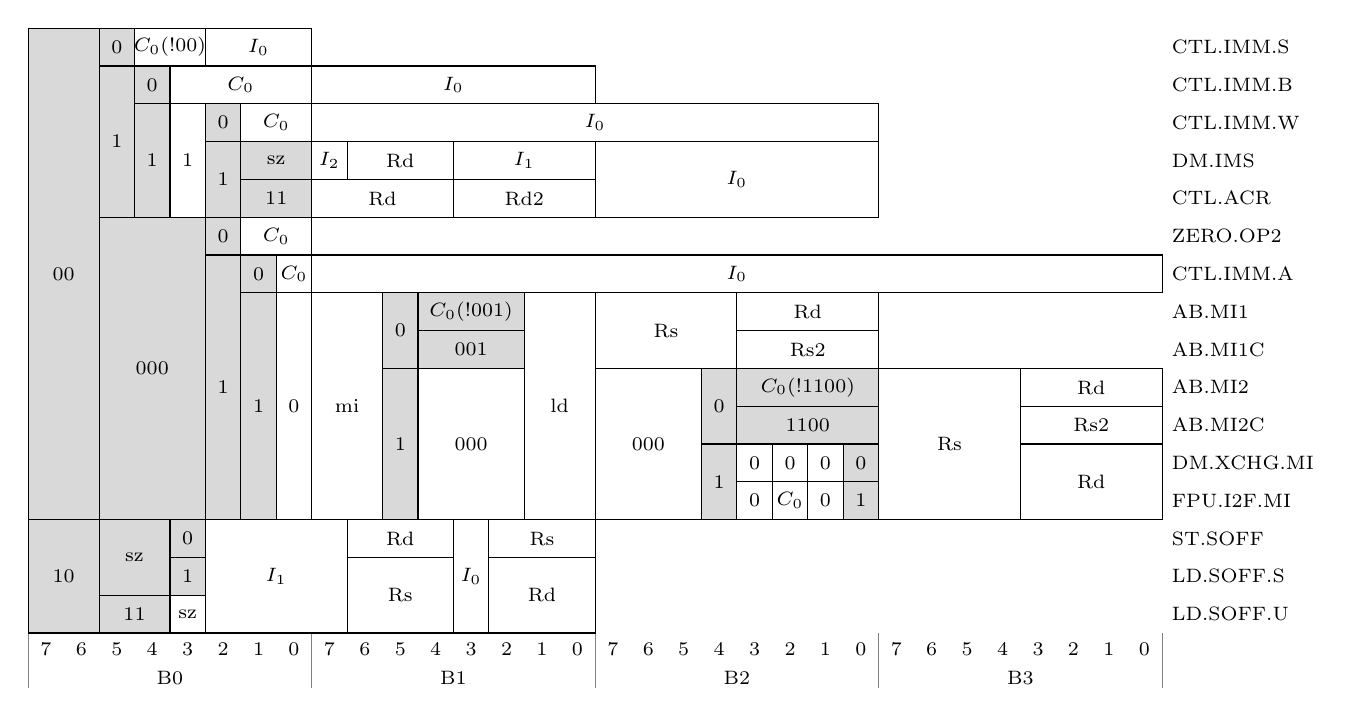
\begin{tikzpicture}[xscale=0.45,yscale=0.24]
\foreach \x in {0, 1, ..., 31}
    \draw (\x + 0.5, 1) node[anchor=north] {\scriptsize \pgfmathparse{int(7 - mod(\x, 8))}\pgfmathresult};
\draw (4, -0.5) node[anchor=north] {\scriptsize B0};
\draw (12, -0.5) node[anchor=north] {\scriptsize B1};
\draw (20, -0.5) node[anchor=north] {\scriptsize B2};
\draw (28, -0.5) node[anchor=north] {\scriptsize B3};
\foreach \x in {0, 8, 16, 24, 32}
    \draw[gray] (\x, -1.9) -- (\x, 1);

% Encoding
% B0(7)
\fill[black!15] (0, \fpuitwoftwop * 2 + 1) rectangle (2, \ctlimmsp * 2 + 3);
\draw (0, \fpuitwoftwop * 2 + 1) rectangle (2, \ctlimmsp * 2 + 3) node[pos=.5] {\scriptsize 00};
\fill[black!15] (0, \ldsoffup * 2 + 1) rectangle (2, \stsoffp * 2 + 3);
\draw (0, \ldsoffup * 2 + 1) rectangle (2, \stsoffp * 2 + 3) node[pos=.5] {\scriptsize 10};
% B0(5)
\fill[black!15] (2, \ctlimmsp * 2 + 1) rectangle (3, \ctlimmsp * 2 + 3);
\draw (2, \ctlimmsp * 2 + 1) rectangle (3, \ctlimmsp * 2 + 3) node[pos=.5] {\scriptsize 0};
\fill[black!15] (2, \ctlacrp * 2 + 1) rectangle (3, \ctlimmbp * 2 + 3);
\draw (2, \ctlacrp * 2 + 1) rectangle (3, \ctlimmbp * 2 + 3) node[pos=.5] {\scriptsize 1};
\fill[black!15] (2, \fpuitwoftwop * 2 + 1) rectangle (5, \zerooptwop * 2 + 3);
\draw (2, \fpuitwoftwop * 2 + 1) rectangle (5, \zerooptwop * 2 + 3) node[pos=.5] {\scriptsize 000};
\fill[black!15] (2, \ldsoffsp * 2 + 1) rectangle (4, \stsoffp * 2 + 3);
\draw (2, \ldsoffsp * 2 + 1) rectangle (4, \stsoffp * 2 + 3) node[pos=.5] {\scriptsize sz};
\fill[black!15] (2, \ldsoffup * 2 + 1) rectangle (4, \ldsoffup * 2 + 3);
\draw (2, \ldsoffup * 2 + 1) rectangle (4, \ldsoffup * 2 + 3) node[pos=.5] {\scriptsize 11};
% B0(4)
\draw (3, \ctlimmsp * 2 + 1) rectangle (5, \ctlimmsp * 2 + 3) node[pos=.5] {\scriptsize $C_0$(!00)};
\fill[black!15] (3, \ctlimmbp * 2 + 1) rectangle (4, \ctlimmbp * 2 + 3);
\draw (3, \ctlimmbp * 2 + 1) rectangle (4, \ctlimmbp * 2 + 3) node[pos=.5] {\scriptsize 0};
\fill[black!15] (3, \ctlacrp * 2 + 1) rectangle (4, \ctlimmwp * 2 + 3);
\draw (3, \ctlacrp * 2 + 1) rectangle (4, \ctlimmwp * 2 + 3) node[pos=.5] {\scriptsize 1};
% B0(3)
\draw (4, \ctlimmbp * 2 + 1) rectangle (8, \ctlimmbp * 2 + 3) node[pos=.5] {\scriptsize $C_0$};
%\fill[black!15] (4, \ctlacrp * 2 + 1) rectangle (5, \ctlimmwp * 2 + 3);
\draw (4, \ctlacrp * 2 + 1) rectangle (5, \ctlimmwp * 2 + 3) node[pos=.5] {\scriptsize 1};
\fill[black!15] (4, \stsoffp * 2 + 1) rectangle (5, \stsoffp * 2 + 3);
\draw (4, \stsoffp * 2 + 1) rectangle (5, \stsoffp * 2 + 3) node[pos=.5] {\scriptsize 0};
\fill[black!15] (4, \ldsoffsp * 2 + 1) rectangle (5, \ldsoffsp * 2 + 3);
\draw (4, \ldsoffsp * 2 + 1) rectangle (5, \ldsoffsp * 2 + 3) node[pos=.5] {\scriptsize 1};
\draw (4, \ldsoffup * 2 + 1) rectangle (5, \ldsoffup * 2 + 3) node[pos=.5] {\scriptsize sz};
% B0(2)
\draw (5, \ctlimmsp * 2 + 1) rectangle (8, \ctlimmsp * 2 + 3) node[pos=.5] {\scriptsize $I_0$};
\fill[black!15] (5, \ctlimmwp * 2 + 1) rectangle (6, \ctlimmwp * 2 + 3);
\draw (5, \ctlimmwp * 2 + 1) rectangle (6, \ctlimmwp * 2 + 3) node[pos=.5] {\scriptsize 0};
\fill[black!15] (5, \ctlacrp * 2 + 1) rectangle (6, \dmimsp * 2 + 3);
\draw (5, \ctlacrp * 2 + 1) rectangle (6, \dmimsp * 2 + 3) node[pos=.5] {\scriptsize 1};
\fill[black!15] (5, \zerooptwop * 2 + 1) rectangle (6, \zerooptwop * 2 + 3);
\draw (5, \zerooptwop * 2 + 1) rectangle (6, \zerooptwop * 2 + 3) node[pos=.5] {\scriptsize 0};
\fill[black!15] (5, \fpuitwoftwop * 2 + 1) rectangle (6, \ctlimmap * 2 + 3);
\draw (5, \fpuitwoftwop * 2 + 1) rectangle (6, \ctlimmap * 2 + 3) node[pos=.5] {\scriptsize 1};
\draw (5, \ldsoffup * 2 + 1) rectangle (9, \stsoffp * 2 + 3) node[pos=.5] {\scriptsize $I_1$};
% B0(1)
\draw (6, \ctlimmwp * 2 + 1) rectangle (8, \ctlimmwp * 2 + 3) node[pos=.5] {\scriptsize $C_0$};
\fill[black!15] (6, \dmimsp * 2 + 1) rectangle (8, \dmimsp * 2 + 3);
\draw (6, \dmimsp * 2 + 1) rectangle (8, \dmimsp * 2 + 3) node[pos=.5] {\scriptsize sz};
\fill[black!15] (6, \ctlacrp * 2 + 1) rectangle (8, \ctlacrp * 2 + 3);
\draw (6, \ctlacrp * 2 + 1) rectangle (8, \ctlacrp * 2 + 3) node[pos=.5] {\scriptsize 11};
\draw (6, \zerooptwop * 2 + 1) rectangle (8, \zerooptwop * 2 + 3) node[pos=.5] {\scriptsize $C_0$};
\fill[black!15] (6, \ctlimmap * 2 + 1) rectangle (7, \ctlimmap * 2 + 3);
\draw (6, \ctlimmap * 2 + 1) rectangle (7, \ctlimmap * 2 + 3) node[pos=.5] {\scriptsize 0};
\fill[black!15] (6, \fpuitwoftwop * 2 + 1) rectangle (7, \iaabmionep * 2 + 3);
\draw (6, \fpuitwoftwop * 2 + 1) rectangle (7, \iaabmionep * 2 + 3) node[pos=.5] {\scriptsize 1};
% B0(0)
\draw (7, \ctlimmap * 2 + 1) rectangle (8, \ctlimmap * 2 + 3) node[pos=.5] {\scriptsize $C_0$};
\draw (7, \fpuitwoftwop * 2 + 1) rectangle (8, \iaabmionep * 2 + 3) node[pos=.5] {\scriptsize 0};
% B1(7)
\draw (8, \ctlimmbp * 2 + 1) rectangle (16, \ctlimmbp * 2 + 3) node[pos=.5] {\scriptsize $I_0$};
\draw (8, \ctlimmwp * 2 + 1) rectangle (24, \ctlimmwp * 2 + 3) node[pos=.5] {\scriptsize $I_0$};
\draw (8, \dmimsp * 2 + 1) rectangle (9, \dmimsp * 2 + 3) node[pos=.5] {\scriptsize $I_2$};
\draw (8, \ctlacrp * 2 + 1) rectangle (12, \ctlacrp * 2 + 3) node[pos=.5] {\scriptsize Rd};
\draw (8, \ctlimmap * 2 + 1) rectangle (32, \ctlimmap * 2 + 3) node[pos=.5] {\scriptsize $I_0$};
\draw (8, \fpuitwoftwop * 2 + 1) rectangle (10, \iaabmionep * 2 + 3) node[pos=.5] {\scriptsize mi};
% B1(6)
\draw (9, \dmimsp * 2 + 1) rectangle (12, \dmimsp * 2 + 3) node[pos=.5] {\scriptsize Rd};
\draw (9, \stsoffp * 2 + 1) rectangle (12, \stsoffp * 2 + 3) node[pos=.5] {\scriptsize Rd};
\draw (9, \ldsoffup * 2 + 1) rectangle (12, \ldsoffsp * 2 + 3) node[pos=.5] {\scriptsize Rs};
% B1(5)
\fill[black!15] (10, \iaabmionecp * 2 + 1) rectangle (11, \iaabmionep * 2 + 3);
\draw (10, \iaabmionecp * 2 + 1) rectangle (11, \iaabmionep * 2 + 3) node[pos=.5] {\scriptsize 0};
\fill[black!15] (10, \fpuitwoftwop * 2 + 1) rectangle (11, \iaabmitwop * 2 + 3);
\draw (10, \fpuitwoftwop * 2 + 1) rectangle (11, \iaabmitwop * 2 + 3) node[pos=.5] {\scriptsize 1};
% B1(4)
\fill[black!15] (11, \iaabmionep * 2 + 1) rectangle (14, \iaabmionep * 2 + 3);
\draw (11, \iaabmionep * 2 + 1) rectangle (14, \iaabmionep * 2 + 3) node[pos=.5] {\scriptsize $C_0$(!001)};
\fill[black!15] (11, \iaabmionecp * 2 + 1) rectangle (14, \iaabmionecp * 2 + 3);
\draw (11, \iaabmionecp * 2 + 1) rectangle (14, \iaabmionecp * 2 + 3) node[pos=.5] {\scriptsize 001};
\draw (11, \fpuitwoftwop * 2 + 1) rectangle (14, \iaabmitwop * 2 + 3) node[pos=.5] {\scriptsize 000};
% B1(3)
\draw (12, \dmimsp * 2 + 1) rectangle (16, \dmimsp * 2 + 3) node[pos=.5] {\scriptsize $I_1$};
\draw (12, \ctlacrp * 2 + 1) rectangle (16, \ctlacrp * 2 + 3) node[pos=.5] {\scriptsize Rd2};
\draw (12, \ldsoffup * 2 + 1) rectangle (13, \stsoffp * 2 + 3) node[pos=.5] {\scriptsize $I_0$};
% B1(2)
\draw (13, \stsoffp * 2 + 1) rectangle (16, \stsoffp * 2 + 3) node[pos=.5] {\scriptsize Rs};
\draw (13, \ldsoffup * 2 + 1) rectangle (16, \ldsoffsp * 2 + 3) node[pos=.5] {\scriptsize Rd};
% B1(1)
\draw (14, \fpuitwoftwop * 2 + 1) rectangle (16, \iaabmionep * 2 + 3) node[pos=.5] {\scriptsize ld};
% B2(7)
\draw (16, \ctlacrp * 2 + 1) rectangle (24, \dmimsp * 2 + 3) node[pos=.5] {\scriptsize $I_0$};
\draw (16, \iaabmionecp * 2 + 1) rectangle (20, \iaabmionep * 2 + 3) node[pos=.5] {\scriptsize Rs};
\draw (16, \fpuitwoftwop * 2 + 1) rectangle (19, \iaabmitwop * 2 + 3) node[pos=.5] {\scriptsize 000};
% B2(4)
\fill[black!15] (19, \iaabmitwocp * 2 + 1) rectangle (20, \iaabmitwop * 2 + 3);
\draw (19, \iaabmitwocp * 2 + 1) rectangle (20, \iaabmitwop * 2 + 3) node[pos=.5] {\scriptsize 0};
\fill[black!15] (19, \fpuitwoftwop * 2 + 1) rectangle (20, \dmxchgmip * 2 + 3);
\draw (19, \fpuitwoftwop * 2 + 1) rectangle (20, \dmxchgmip * 2 + 3) node[pos=.5] {\scriptsize 1};
% B2(3)
\draw (20, \iaabmionep * 2 + 1) rectangle (24, \iaabmionep * 2 + 3) node[pos=.5] {\scriptsize Rd};
\draw (20, \iaabmionecp * 2 + 1) rectangle (24, \iaabmionecp * 2 + 3) node[pos=.5] {\scriptsize Rs2};
\fill[black!15] (20, \iaabmitwop * 2 + 1) rectangle (24, \iaabmitwop * 2 + 3);
\draw (20, \iaabmitwop * 2 + 1) rectangle (24, \iaabmitwop * 2 + 3) node[pos=.5] {\scriptsize $C_0$(!1100)};
\fill[black!15] (20, \iaabmitwocp * 2 + 1) rectangle (24, \iaabmitwocp * 2 + 3);
\draw (20, \iaabmitwocp * 2 + 1) rectangle (24, \iaabmitwocp * 2 + 3) node[pos=.5] {\scriptsize 1100};
\draw (20, \dmxchgmip * 2 + 1) rectangle (21, \dmxchgmip * 2 + 3) node[pos=.5] {\scriptsize 0};
\draw (20, \fpuitwoftwop * 2 + 1) rectangle (21, \fpuitwoftwop * 2 + 3) node[pos=.5] {\scriptsize 0};
% B2(2)
\draw (21, \dmxchgmip * 2 + 1) rectangle (22, \dmxchgmip * 2 + 3) node[pos=.5] {\scriptsize 0};
\draw (21, \fpuitwoftwop * 2 + 1) rectangle (22, \fpuitwoftwop * 2 + 3) node[pos=.5] {\scriptsize $C_0$};
% B2(1)
\draw (22, \dmxchgmip * 2 + 1) rectangle (23, \dmxchgmip * 2 + 3) node[pos=.5] {\scriptsize 0};
\draw (22, \fpuitwoftwop * 2 + 1) rectangle (23, \fpuitwoftwop * 2 + 3) node[pos=.5] {\scriptsize 0};
% B2(0)
\fill[black!15] (23, \dmxchgmip * 2 + 1) rectangle (24, \dmxchgmip * 2 + 3);
\draw (23, \dmxchgmip * 2 + 1) rectangle (24, \dmxchgmip * 2 + 3) node[pos=.5] {\scriptsize 0};
\fill[black!15] (23, \fpuitwoftwop * 2 + 1) rectangle (24, \fpuitwoftwop * 2 + 3);
\draw (23, \fpuitwoftwop * 2 + 1) rectangle (24, \fpuitwoftwop * 2 + 3) node[pos=.5] {\scriptsize 1};
% B3(7)
\draw (24, \fpuitwoftwop * 2 + 1) rectangle (28, \iaabmitwop * 2 + 3) node[pos=.5] {\scriptsize Rs};
% B3(3)
\draw (28, \iaabmitwop * 2 + 1) rectangle (32, \iaabmitwop * 2 + 3) node[pos=.5] {\scriptsize Rd};
\draw (28, \iaabmitwocp * 2 + 1) rectangle (32, \iaabmitwocp * 2 + 3) node[pos=.5] {\scriptsize Rs2};
\draw (28, \fpuitwoftwop * 2 + 1) rectangle (32, \dmxchgmip * 2 + 3) node[pos=.5] {\scriptsize Rd};

% Group names
\draw (32, \ctlimmsp * 2 + 2) node[anchor=west] {\scriptsize CTL.IMM.S};
\draw (32, \ctlimmbp * 2 + 2) node[anchor=west] {\scriptsize CTL.IMM.B};
\draw (32, \ctlimmwp * 2 + 2) node[anchor=west] {\scriptsize CTL.IMM.W};
\draw (32, \dmimsp * 2 + 2) node[anchor=west] {\scriptsize DM.IMS};
\draw (32, \ctlacrp * 2 + 2) node[anchor=west] {\scriptsize CTL.ACR};
\draw (32, \zerooptwop * 2 + 2) node[anchor=west] {\scriptsize ZERO.OP2};
\draw (32, \ctlimmap * 2 + 2) node[anchor=west] {\scriptsize CTL.IMM.A};
\draw (32, \iaabmionep * 2 + 2) node[anchor=west] {\scriptsize AB.MI1};
\draw (32, \iaabmionecp * 2 + 2) node[anchor=west] {\scriptsize AB.MI1C};
\draw (32, \iaabmitwop * 2 + 2) node[anchor=west] {\scriptsize AB.MI2};
\draw (32, \iaabmitwocp * 2 + 2) node[anchor=west] {\scriptsize AB.MI2C};
\draw (32, \dmxchgmip * 2 + 2) node[anchor=west] {\scriptsize DM.XCHG.MI};
\draw (32, \fpuitwoftwop * 2 + 2) node[anchor=west] {\scriptsize FPU.I2F.MI};
\draw (32, \stsoffp * 2 + 2) node[anchor=west] {\scriptsize ST.SOFF};
\draw (32, \ldsoffsp * 2 + 2) node[anchor=west] {\scriptsize LD.SOFF.S};
\draw (32, \ldsoffup * 2 + 2) node[anchor=west] {\scriptsize LD.SOFF.U};
\end{tikzpicture}
\captionsetup{font=scriptsize, labelfont=scriptsize}
\caption{RX Instruction Encoding Part 1 of 4. sz $\ne$ 11 when its width is 2 bits.}
\figlabel{CArch.Summary.ISA.RX.IEncoding.PartI}
\end{subfigure}

\vspace{0.5cm}

\begin{subfigure}{\linewidth}
\centering
\newcommand{\dmmmp}{21}
\newcommand{\stoffp}{20}
\newcommand{\ldoffsp}{19}
\newcommand{\dmrrp}{18}
\newcommand{\bmimonep}{17}
\newcommand{\bmimtwop}{16}
\newcommand{\dmstksimp}{15}
\newcommand{\dmimp}{14}
\newcommand{\dmirp}{13}
\newcommand{\dpurtlip}{12}
\newcommand{\dpurthip}{11}
\newcommand{\iaabldtwop}{10}
\newcommand{\iaabldtwocp}{9}
\newcommand{\dmxchgldp}{8}
\newcommand{\fpuitwofonep}{7}
\newcommand{\dmcmovp}{6}
\newcommand{\bmrngp}{5}
\newcommand{\bmregp}{4}
\newcommand{\bmregcp}{3}
\newcommand{\dpustp}{2}
\newcommand{\fpuldp}{1}
\newcommand{\fpuldcp}{0}

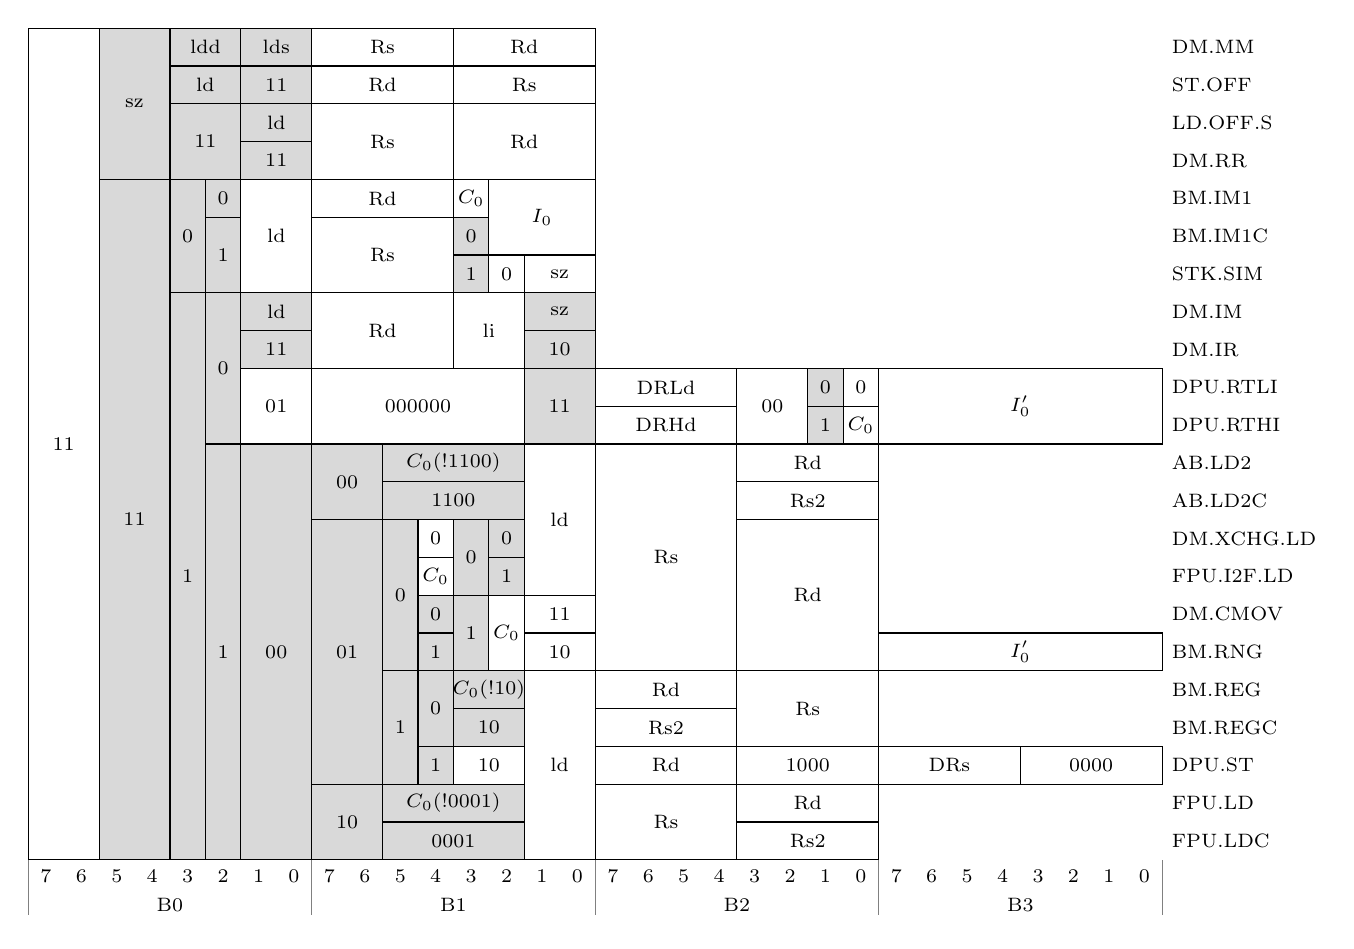
\begin{tikzpicture}[xscale=0.45,yscale=0.24]
\foreach \x in {0, 1, ..., 31}
    \draw (\x + 0.5, 1) node[anchor=north] {\scriptsize \pgfmathparse{int(7 - mod(\x, 8))}\pgfmathresult};
\draw (4, -0.5) node[anchor=north] {\scriptsize B0};
\draw (12, -0.5) node[anchor=north] {\scriptsize B1};
\draw (20, -0.5) node[anchor=north] {\scriptsize B2};
\draw (28, -0.5) node[anchor=north] {\scriptsize B3};
\foreach \x in {0, 8, 16, 24, 32}
    \draw[gray] (\x, -1.9) -- (\x, 1);

% Encoding
% B0(7)
\draw (0, \fpuldcp * 2 + 1) rectangle (2, \dmmmp * 2 + 3) node[pos=.5] {\scriptsize 11};

% B0(5)
\fill[black!15] (2, \dmrrp * 2 + 1) rectangle (4, \dmmmp * 2 + 3);
\draw (2, \dmrrp * 2 + 1) rectangle (4, \dmmmp * 2 + 3) node[pos=.5] {\scriptsize sz};
\fill[black!15] (2, \fpuldcp * 2 + 1) rectangle (4, \bmimonep * 2 + 3);
\draw (2, \fpuldcp * 2 + 1) rectangle (4, \bmimonep * 2 + 3) node[pos=.5] {\scriptsize 11};

% B0(3)
\fill[black!15] (4, \dmmmp * 2 + 1) rectangle (6, \dmmmp * 2 + 3);
\draw (4, \dmmmp * 2 + 1) rectangle (6, \dmmmp * 2 + 3) node[pos=.5] {\scriptsize ldd};
\fill[black!15] (4, \stoffp * 2 + 1) rectangle (6, \stoffp * 2 + 3);
\draw (4, \stoffp * 2 + 1) rectangle (6, \stoffp * 2 + 3) node[pos=.5] {\scriptsize ld};
\fill[black!15] (4, \dmrrp * 2 + 1) rectangle (6, \ldoffsp * 2 + 3);
\draw (4, \dmrrp * 2 + 1) rectangle (6, \ldoffsp * 2 + 3) node[pos=.5] {\scriptsize 11};
\fill[black!15] (4, \dmstksimp * 2 + 1) rectangle (5, \bmimonep * 2 + 3);
\draw (4, \dmstksimp * 2 + 1) rectangle (5, \bmimonep * 2 + 3) node[pos=.5] {\scriptsize 0};
\fill[black!15] (4, \fpuldcp * 2 + 1) rectangle (5, \dmimp * 2 + 3);
\draw (4, \fpuldcp * 2 + 1) rectangle (5, \dmimp * 2 + 3) node[pos=.5] {\scriptsize 1};

% B0(2)
\fill[black!15] (5, \bmimonep * 2 + 1) rectangle (6, \bmimonep * 2 + 3);
\draw (5, \bmimonep * 2 + 1) rectangle (6, \bmimonep * 2 + 3) node[pos=.5] {\scriptsize 0};
\fill[black!15] (5, \dmstksimp * 2 + 1) rectangle (6, \bmimtwop * 2 + 3);
\draw (5, \dmstksimp * 2 + 1) rectangle (6, \bmimtwop * 2 + 3) node[pos=.5] {\scriptsize 1};
\fill[black!15] (5, \dpurthip * 2 + 1) rectangle (6, \dmimp * 2 + 3);
\draw (5, \dpurthip * 2 + 1) rectangle (6, \dmimp * 2 + 3) node[pos=.5] {\scriptsize 0};
\fill[black!15] (5, \fpuldcp * 2 + 1) rectangle (6, \iaabldtwop * 2 + 3);
\draw (5, \fpuldcp * 2 + 1) rectangle (6, \iaabldtwop * 2 + 3) node[pos=.5] {\scriptsize 1};

% B0(1)
\fill[black!15] (6, \dmmmp * 2 + 1) rectangle (8, \dmmmp * 2 + 3);
\draw (6, \dmmmp * 2 + 1) rectangle (8, \dmmmp * 2 + 3) node[pos=.5] {\scriptsize lds};
\fill[black!15] (6, \stoffp * 2 + 1) rectangle (8, \stoffp * 2 + 3);
\draw (6, \stoffp * 2 + 1) rectangle (8, \stoffp * 2 + 3) node[pos=.5] {\scriptsize 11};
\fill[black!15] (6, \ldoffsp * 2 + 1) rectangle (8, \ldoffsp * 2 + 3);
\draw (6, \ldoffsp * 2 + 1) rectangle (8, \ldoffsp * 2 + 3) node[pos=.5] {\scriptsize ld};
\fill[black!15] (6, \dmrrp * 2 + 1) rectangle (8, \dmrrp * 2 + 3);
\draw (6, \dmrrp * 2 + 1) rectangle (8, \dmrrp * 2 + 3) node[pos=.5] {\scriptsize 11};
\draw (6, \dmstksimp * 2 + 1) rectangle (8, \bmimonep * 2 + 3) node[pos=.5] {\scriptsize ld};
\fill[black!15] (6, \dmimp * 2 + 1) rectangle (8, \dmimp * 2 + 3);
\draw (6, \dmimp * 2 + 1) rectangle (8, \dmimp * 2 + 3) node[pos=.5] {\scriptsize ld};
\fill[black!15] (6, \dmirp * 2 + 1) rectangle (8, \dmirp * 2 + 3);
\draw (6, \dmirp * 2 + 1) rectangle (8, \dmirp * 2 + 3) node[pos=.5] {\scriptsize 11};
\draw (6, \dpurthip * 2 + 1) rectangle (8, \dpurtlip * 2 + 3) node[pos=.5] {\scriptsize 01};
\fill[black!15] (6, \fpuldcp * 2 + 1) rectangle (8, \iaabldtwop * 2 + 3);
\draw (6, \fpuldcp * 2 + 1) rectangle (8, \iaabldtwop * 2 + 3) node[pos=.5] {\scriptsize 00};

% B1(7)
\draw (8, \dmmmp * 2 + 1) rectangle (12, \dmmmp * 2 + 3) node[pos=.5] {\scriptsize Rs};
\draw (8, \stoffp * 2 + 1) rectangle (12, \stoffp * 2 + 3) node[pos=.5] {\scriptsize Rd};
\draw (8, \dmrrp * 2 + 1) rectangle (12, \ldoffsp * 2 + 3) node[pos=.5] {\scriptsize Rs};
\draw (8, \bmimonep * 2 + 1) rectangle (12, \bmimonep * 2 + 3) node[pos=.5] {\scriptsize Rd};
\draw (8, \dmstksimp * 2 + 1) rectangle (12, \bmimtwop * 2 + 3) node[pos=.5] {\scriptsize Rs};
\draw (8, \dmirp * 2 + 1) rectangle (12, \dmimp * 2 + 3) node[pos=.5] {\scriptsize Rd};
\draw (8, \dpurthip * 2 + 1) rectangle (14, \dpurtlip * 2 + 3) node[pos=.5] {\scriptsize 000000};
\fill[black!15] (8, \iaabldtwocp * 2 + 1) rectangle (10, \iaabldtwop * 2 + 3);
\draw (8, \iaabldtwocp * 2 + 1) rectangle (10, \iaabldtwop * 2 + 3) node[pos=.5] {\scriptsize 00};
\fill[black!15] (8, \dpustp * 2 + 1) rectangle (10, \dmxchgldp * 2 + 3);
\draw (8, \dpustp * 2 + 1) rectangle (10, \dmxchgldp * 2 + 3) node[pos=.5] {\scriptsize 01};
\fill[black!15] (8, \fpuldcp * 2 + 1) rectangle (10, \fpuldp * 2 + 3);
\draw (8, \fpuldcp * 2 + 1) rectangle (10, \fpuldp * 2 + 3) node[pos=.5] {\scriptsize 10};

% B1(5)
\fill[black!15] (10, \iaabldtwop * 2 + 1) rectangle (14, \iaabldtwop * 2 + 3);
\draw (10, \iaabldtwop * 2 + 1) rectangle (14, \iaabldtwop * 2 + 3) node[pos=.5] {\scriptsize $C_0$(!1100)};
\fill[black!15] (10, \iaabldtwocp * 2 + 1) rectangle (14, \iaabldtwocp * 2 + 3);
\draw (10, \iaabldtwocp * 2 + 1) rectangle (14, \iaabldtwocp * 2 + 3) node[pos=.5] {\scriptsize 1100};
\fill[black!15] (10, \bmrngp * 2 + 1) rectangle (11, \dmxchgldp * 2 + 3);
\draw (10, \bmrngp * 2 + 1) rectangle (11, \dmxchgldp * 2 + 3) node[pos=.5] {\scriptsize 0};
\fill[black!15] (10, \dpustp * 2 + 1) rectangle (11, \bmregp * 2 + 3);
\draw (10, \dpustp * 2 + 1) rectangle (11, \bmregp * 2 + 3) node[pos=.5] {\scriptsize 1};
\fill[black!15] (10, \fpuldp * 2 + 1) rectangle (14, \fpuldp * 2 + 3);
\draw (10, \fpuldp * 2 + 1) rectangle (14, \fpuldp * 2 + 3) node[pos=.5] {\scriptsize $C_0$(!0001)};
\fill[black!15] (10, \fpuldcp * 2 + 1) rectangle (14, \fpuldcp * 2 + 3);
\draw (10, \fpuldcp * 2 + 1) rectangle (14, \fpuldcp * 2 + 3) node[pos=.5] {\scriptsize 0001};

% B1(4)
\draw (11, \dmxchgldp * 2 + 1) rectangle (12, \dmxchgldp * 2 + 3) node[pos=.5] {\scriptsize 0};
\draw (11, \fpuitwofonep * 2 + 1) rectangle (12, \fpuitwofonep * 2 + 3) node[pos=.5] {\scriptsize $C_0$};
\fill[black!15] (11, \dmcmovp * 2 + 1) rectangle (12, \dmcmovp * 2 + 3);
\draw (11, \dmcmovp * 2 + 1) rectangle (12, \dmcmovp * 2 + 3) node[pos=.5] {\scriptsize 0};
\fill[black!15] (11, \bmrngp * 2 + 1) rectangle (12, \bmrngp * 2 + 3);
\draw (11, \bmrngp * 2 + 1) rectangle (12, \bmrngp * 2 + 3) node[pos=.5] {\scriptsize 1};
\fill[black!15] (11, \bmregcp * 2 + 1) rectangle (12, \bmregp * 2 + 3);
\draw (11, \bmregcp * 2 + 1) rectangle (12, \bmregp * 2 + 3) node[pos=.5] {\scriptsize 0};
\fill[black!15] (11, \dpustp * 2 + 1) rectangle (12, \dpustp * 2 + 3);
\draw (11, \dpustp * 2 + 1) rectangle (12, \dpustp * 2 + 3) node[pos=.5] {\scriptsize 1};

% B1(3)
\draw (12, \dmmmp * 2 + 1) rectangle (16, \dmmmp * 2 + 3) node[pos=.5] {\scriptsize Rd};
\draw (12, \stoffp * 2 + 1) rectangle (16, \stoffp * 2 + 3) node[pos=.5] {\scriptsize Rs};
\draw (12, \dmrrp * 2 + 1) rectangle (16, \ldoffsp * 2 + 3) node[pos=.5] {\scriptsize Rd};
\draw (12, \bmimonep * 2 + 1) rectangle (13, \bmimonep * 2 + 3) node[pos=.5] {\scriptsize $C_0$};
\fill[black!15] (12, \bmimtwop * 2 + 1) rectangle (13, \bmimtwop * 2 + 3);
\draw (12, \bmimtwop * 2 + 1) rectangle (13, \bmimtwop * 2 + 3) node[pos=.5] {\scriptsize 0};
\fill[black!15] (12, \dmstksimp * 2 + 1) rectangle (13, \dmstksimp * 2 + 3);
\draw (12, \dmstksimp * 2 + 1) rectangle (13, \dmstksimp * 2 + 3) node[pos=.5] {\scriptsize 1};
\draw (12, \dmirp * 2 + 1) rectangle (14, \dmimp * 2 + 3) node[pos=.5] {\scriptsize li};
\fill[black!15] (12, \fpuitwofonep * 2 + 1) rectangle (13, \dmxchgldp * 2 + 3);
\draw (12, \fpuitwofonep * 2 + 1) rectangle (13, \dmxchgldp * 2 + 3) node[pos=.5] {\scriptsize 0};
\fill[black!15] (12, \bmrngp * 2 + 1) rectangle (13, \dmcmovp * 2 + 3);
\draw (12, \bmrngp * 2 + 1) rectangle (13, \dmcmovp * 2 + 3) node[pos=.5] {\scriptsize 1};
\fill[black!15] (12, \bmregp * 2 + 1) rectangle (14, \bmregp * 2 + 3);
\draw (12, \bmregp * 2 + 1) rectangle (14, \bmregp * 2 + 3) node[pos=.5] {\scriptsize $C_0$(!10)};
\fill[black!15] (12, \bmregcp * 2 + 1) rectangle (14, \bmregcp * 2 + 3);
\draw (12, \bmregcp * 2 + 1) rectangle (14, \bmregcp * 2 + 3) node[pos=.5] {\scriptsize 10};
\draw (12, \dpustp * 2 + 1) rectangle (14, \dpustp * 2 + 3) node[pos=.5] {\scriptsize 10};

% B1(2)
\draw (13, \bmimtwop * 2 + 1) rectangle (16, \bmimonep * 2 + 3) node[pos=.5] {\scriptsize $I_0$};
\draw (13, \dmstksimp * 2 + 1) rectangle (14, \dmstksimp * 2 + 3) node[pos=.5] {\scriptsize 0};
\fill[black!15] (13, \dmxchgldp * 2 + 1) rectangle (14, \dmxchgldp * 2 + 3);
\draw (13, \dmxchgldp * 2 + 1) rectangle (14, \dmxchgldp * 2 + 3) node[pos=.5] {\scriptsize 0};
\fill[black!15] (13, \fpuitwofonep * 2 + 1) rectangle (14, \fpuitwofonep * 2 + 3);
\draw (13, \fpuitwofonep * 2 + 1) rectangle (14, \fpuitwofonep * 2 + 3) node[pos=.5] {\scriptsize 1};
\draw (13, \bmrngp * 2 + 1) rectangle (14, \dmcmovp * 2 + 3) node[pos=.5] {\scriptsize $C_0$};

% B1(1)
\draw (14, \dmstksimp * 2 + 1) rectangle (16, \dmstksimp * 2 + 3) node[pos=.5] {\scriptsize sz};
\fill[black!15] (14, \dmimp * 2 + 1) rectangle (16, \dmimp * 2 + 3);
\draw (14, \dmimp * 2 + 1) rectangle (16, \dmimp * 2 + 3) node[pos=.5] {\scriptsize sz};
\fill[black!15] (14, \dmirp * 2 + 1) rectangle (16, \dmirp * 2 + 3);
\draw (14, \dmirp * 2 + 1) rectangle (16, \dmirp * 2 + 3) node[pos=.5] {\scriptsize 10};
\fill[black!15] (14, \dpurthip * 2 + 1) rectangle (16, \dpurtlip * 2 + 3);
\draw (14, \dpurthip * 2 + 1) rectangle (16, \dpurtlip * 2 + 3) node[pos=.5] {\scriptsize 11};
\draw (14, \fpuitwofonep * 2 + 1) rectangle (16, \iaabldtwop * 2 + 3) node[pos=.5] {\scriptsize ld};
\draw (14, \dmcmovp * 2 + 1) rectangle (16, \dmcmovp * 2 + 3) node[pos=.5] {\scriptsize 11};
\draw (14, \bmrngp * 2 + 1) rectangle (16, \bmrngp * 2 + 3) node[pos=.5] {\scriptsize 10};
\draw (14, \fpuldcp * 2 + 1) rectangle (16, \bmregp * 2 + 3) node[pos=.5] {\scriptsize ld};

% B2(7)
\draw (16, \dpurtlip * 2 + 1) rectangle (20, \dpurtlip * 2 + 3) node[pos=.5] {\scriptsize DRLd};
\draw (16, \dpurthip * 2 + 1) rectangle (20, \dpurthip * 2 + 3) node[pos=.5] {\scriptsize DRHd};
\draw (16, \bmrngp * 2 + 1) rectangle (20, \iaabldtwop * 2 + 3) node[pos=.5] {\scriptsize Rs};
\draw (16, \bmregp * 2 + 1) rectangle (20, \bmregp * 2 + 3) node[pos=.5] {\scriptsize Rd};
\draw (16, \bmregcp * 2 + 1) rectangle (20, \bmregcp * 2 + 3) node[pos=.5] {\scriptsize Rs2};
\draw (16, \dpustp * 2 + 1) rectangle (20, \dpustp * 2 + 3) node[pos=.5] {\scriptsize Rd};
\draw (16, \fpuldcp * 2 + 1) rectangle (20, \fpuldp * 2 + 3) node[pos=.5] {\scriptsize Rs};

% B2(3)
\draw (20, \dpurthip * 2 + 1) rectangle (22, \dpurtlip * 2 + 3) node[pos=.5] {\scriptsize 00};
\draw (20, \iaabldtwop * 2 + 1) rectangle (24, \iaabldtwop * 2 + 3) node[pos=.5] {\scriptsize Rd};
\draw (20, \iaabldtwocp * 2 + 1) rectangle (24, \iaabldtwocp * 2 + 3) node[pos=.5] {\scriptsize Rs2};
\draw (20, \bmrngp * 2 + 1) rectangle (24, \dmxchgldp * 2 + 3) node[pos=.5] {\scriptsize Rd};
\draw (20, \bmregcp * 2 + 1) rectangle (24, \bmregp * 2 + 3) node[pos=.5] {\scriptsize Rs};
\draw (20, \dpustp * 2 + 1) rectangle (24, \dpustp * 2 + 3) node[pos=.5] {\scriptsize 1000};
\draw (20, \fpuldp * 2 + 1) rectangle (24, \fpuldp * 2 + 3) node[pos=.5] {\scriptsize Rd};
\draw (20, \fpuldcp * 2 + 1) rectangle (24, \fpuldcp * 2 + 3) node[pos=.5] {\scriptsize Rs2};

% B2(1)
\fill[black!15] (22, \dpurtlip * 2 + 1) rectangle (23, \dpurtlip * 2 + 3);
\draw (22, \dpurtlip * 2 + 1) rectangle (23, \dpurtlip * 2 + 3) node[pos=.5] {\scriptsize 0};
\fill[black!15] (22, \dpurthip * 2 + 1) rectangle (23, \dpurthip * 2 + 3);
\draw (22, \dpurthip * 2 + 1) rectangle (23, \dpurthip * 2 + 3) node[pos=.5] {\scriptsize 1};

% B2(0)
\draw (23, \dpurtlip * 2 + 1) rectangle (24, \dpurtlip * 2 + 3) node[pos=.5] {\scriptsize 0};
\draw (23, \dpurthip * 2 + 1) rectangle (24, \dpurthip * 2 + 3) node[pos=.5] {\scriptsize $C_0$};

% B3(7)
\draw (24, \dpurthip * 2 + 1) rectangle (32, \dpurtlip * 2 + 3) node[pos=.5] {\scriptsize $I_0'$};
\draw (24, \bmrngp * 2 + 1) rectangle (32, \bmrngp * 2 + 3) node[pos=.5] {\scriptsize $I_0'$};
\draw (24, \dpustp * 2 + 1) rectangle (28, \dpustp * 2 + 3) node[pos=.5] {\scriptsize DRs};

% B3(3)
\draw (28, \dpustp * 2 + 1) rectangle (32, \dpustp * 2 + 3) node[pos=.5] {\scriptsize 0000};

% Group names
\draw (32, \dmmmp * 2 + 2) node[anchor=west] {\scriptsize DM.MM};
\draw (32, \stoffp * 2 + 2) node[anchor=west] {\scriptsize ST.OFF};
\draw (32, \ldoffsp * 2 + 2) node[anchor=west] {\scriptsize LD.OFF.S};
\draw (32, \dmrrp * 2 + 2) node[anchor=west] {\scriptsize DM.RR};
\draw (32, \bmimonep * 2 + 2) node[anchor=west] {\scriptsize BM.IM1};
\draw (32, \bmimtwop * 2 + 2) node[anchor=west] {\scriptsize BM.IM1C};
\draw (32, \dmstksimp * 2 + 2) node[anchor=west] {\scriptsize STK.SIM};
\draw (32, \dmimp * 2 + 2) node[anchor=west] {\scriptsize DM.IM};
\draw (32, \dmirp * 2 + 2) node[anchor=west] {\scriptsize DM.IR};
\draw (32, \dpurtlip * 2 + 2) node[anchor=west] {\scriptsize DPU.RTLI};
\draw (32, \dpurthip * 2 + 2) node[anchor=west] {\scriptsize DPU.RTHI};
\draw (32, \iaabldtwop * 2 + 2) node[anchor=west] {\scriptsize AB.LD2};
\draw (32, \iaabldtwocp * 2 + 2) node[anchor=west] {\scriptsize AB.LD2C};
\draw (32, \dmxchgldp * 2 + 2) node[anchor=west] {\scriptsize DM.XCHG.LD};
\draw (32, \fpuitwofonep * 2 + 2) node[anchor=west] {\scriptsize FPU.I2F.LD};
\draw (32, \dmcmovp * 2 + 2) node[anchor=west] {\scriptsize DM.CMOV};
\draw (32, \bmrngp * 2 + 2) node[anchor=west] {\scriptsize BM.RNG};
\draw (32, \bmregp * 2 + 2) node[anchor=west] {\scriptsize BM.REG};
\draw (32, \bmregcp * 2 + 2) node[anchor=west] {\scriptsize BM.REGC};
\draw (32, \dpustp * 2 + 2) node[anchor=west] {\scriptsize DPU.ST};
\draw (32, \fpuldp * 2 + 2) node[anchor=west] {\scriptsize FPU.LD};
\draw (32, \fpuldcp * 2 + 2) node[anchor=west] {\scriptsize FPU.LDC};
\end{tikzpicture}
\captionsetup{font=scriptsize, labelfont=scriptsize}
\caption{RX Instruction Encoding Part 2 of 4. sz $\ne$ 11 when its width is 2 bits. ldd, lds $\ne$ 11 for DM.MM.
ld $\ne$ 11 for ST.OFF, LD.OFF.S and DM.IM instruction groups.}
\figlabel{CArch.Summary.ISA.RX.IEncoding.PartII}
\end{subfigure}

\captionsetup{font=scriptsize, labelfont=scriptsize}
\caption{RX Instruction Encoding Parts 1 and 2. Refer to \protect\SOPNoteRef{CArch.Summary.ISA.RX.Note.4}{Section 4} 
and \protect\SOPNoteRef{CArch.Summary.ISA.RX.Note.7}{Section 7} for details of fields used and constraints on those 
fields.}
\figlabel{CArch.Summary.ISA.RX.IEncoding.PartI.PartII}
\end{figure}

\clearpage
\begin{figure}
\begin{center}
\newcommand{\iaabldonep}{36}
\newcommand{\iaabldonecp}{35}
\newcommand{\ldoffup}{34}
\newcommand{\iaabironecp}{33}
\newcommand{\iaabironep}{32}
\newcommand{\ctlacap}{31}
\newcommand{\iashimmonep}{30}
\newcommand{\dmstkmip}{29}
\newcommand{\dmstkmop}{28}
\newcommand{\iaabirfivep}{27}
\newcommand{\iaabirthreep}{26}
\newcommand{\iaabirthreecp}{25}
\newcommand{\dmirsp}{24}
\newcommand{\iaabirtwocp}{23}
\newcommand{\sysintp}{22}
\newcommand{\sysiplp}{21}
\newcommand{\dpumvfp}{20}
\newcommand{\dpubap}{19}
\newcommand{\dpucmpp}{18}
\newcommand{\dpuuamp}{17}
\newcommand{\dpucfdp}{16}
\newcommand{\dpupushcp}{15}
\newcommand{\dpupopcp}{14}
\newcommand{\dpupushp}{13}
\newcommand{\dpupopp}{12}
\newcommand{\bmironep}{11}
\newcommand{\bmironecp}{10}
\newcommand{\iaabregonep}{9}
\newcommand{\iashcryp}{8}
\newcommand{\dmstksip}{7}
\newcommand{\dmstksop}{6}
\newcommand{\dmstkctlp}{5}
\newcommand{\ctlregp}{4}
\newcommand{\aryszp}{3}
\newcommand{\arybp}{2}
\newcommand{\zerooponep}{1}
\newcommand{\syspswp}{0}

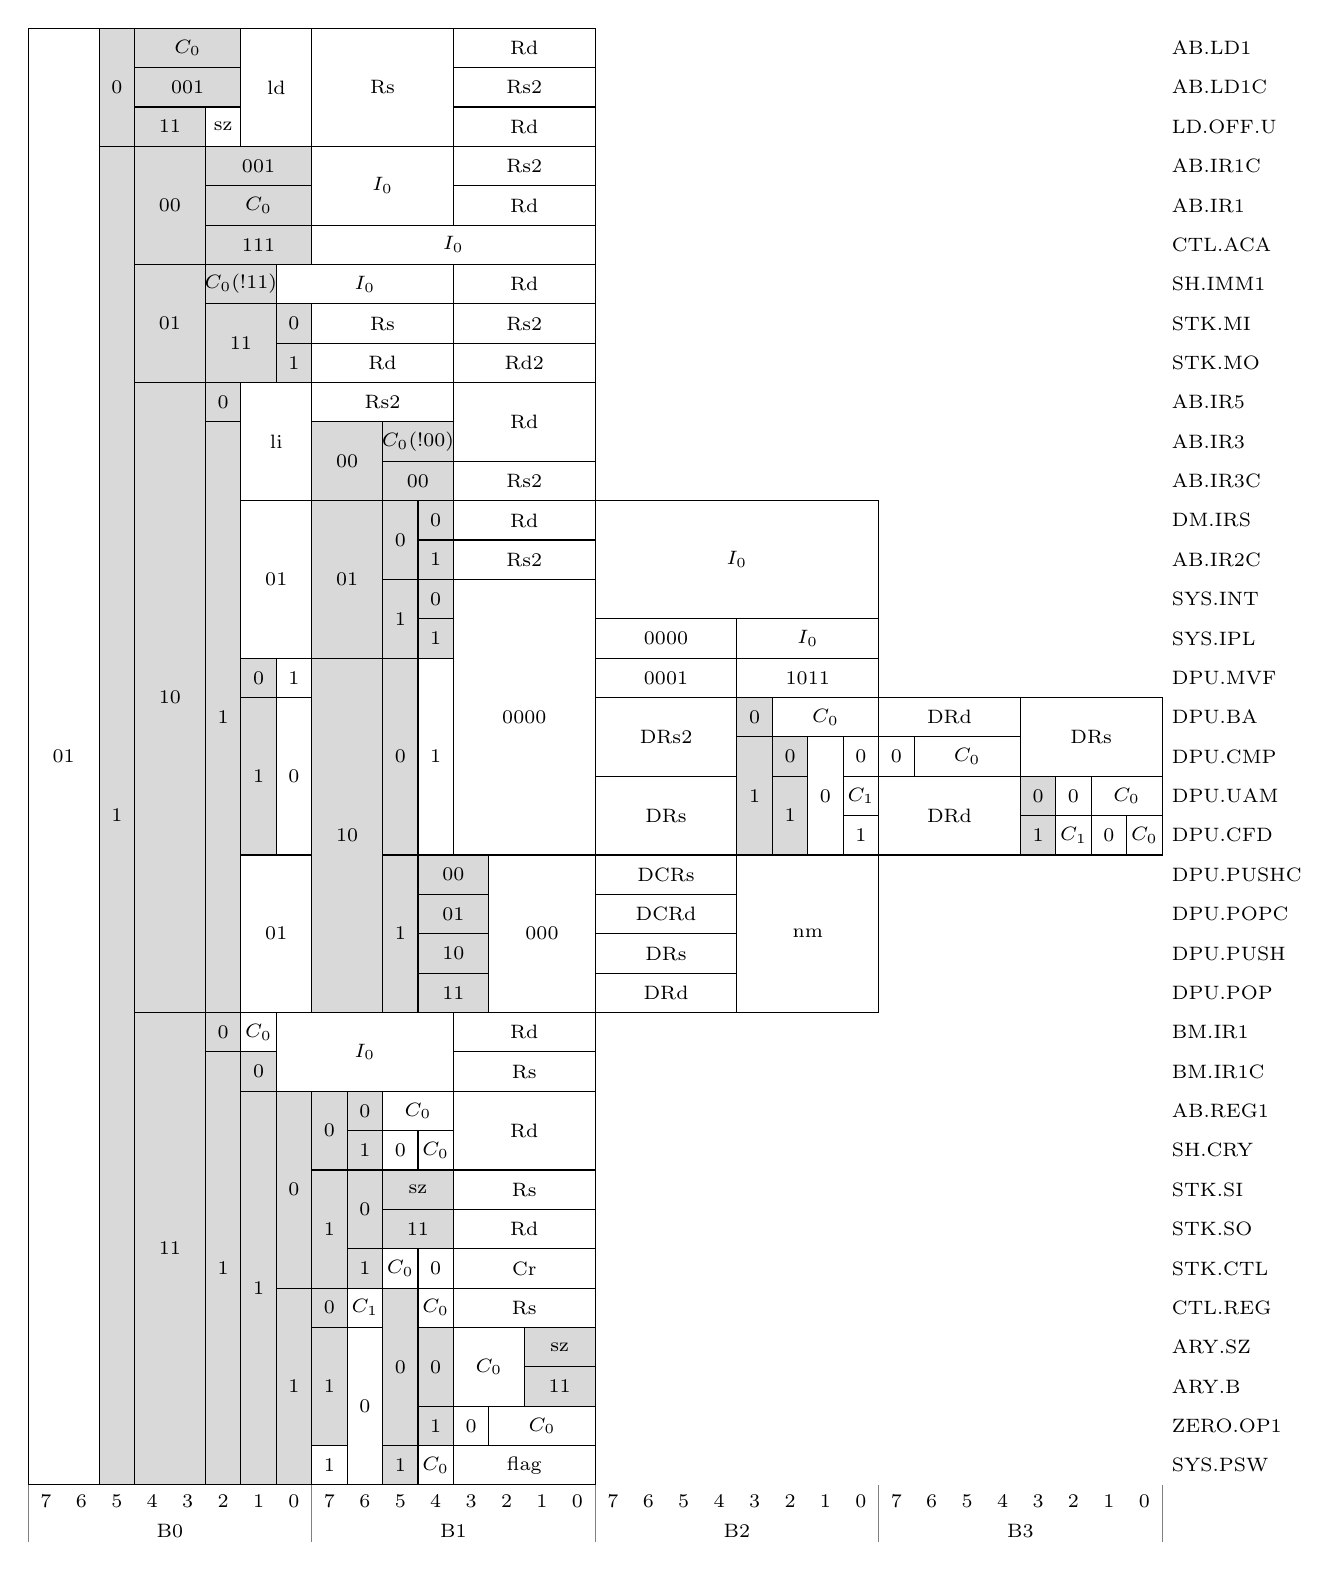
\begin{tikzpicture}[xscale=0.45,yscale=0.25]
\foreach \x in {0, 1, ..., 31}
    \draw (\x + 0.5, 1) node[anchor=north] {\scriptsize \pgfmathparse{int(7 - mod(\x, 8))}\pgfmathresult};
\draw (4, -0.5) node[anchor=north] {\scriptsize B0};
\draw (12, -0.5) node[anchor=north] {\scriptsize B1};
\draw (20, -0.5) node[anchor=north] {\scriptsize B2};
\draw (28, -0.5) node[anchor=north] {\scriptsize B3};
\foreach \x in {0, 8, 16, 24, 32}
    \draw[gray] (\x, -1.9) -- (\x, 1);

% Encoding
% B0(7)
\draw (0, \syspswp * 2 + 1) rectangle (2, \iaabldonep * 2 + 3) node[pos=.5] {\scriptsize 01};

% B0(5)
\fill[black!15] (2, \ldoffup * 2 + 1) rectangle (3, \iaabldonep * 2 + 3);
\draw (2, \ldoffup * 2 + 1) rectangle (3, \iaabldonep * 2 + 3) node[pos=.5] {\scriptsize 0};
\fill[black!15] (2, \syspswp * 2 + 1) rectangle (3, \iaabironecp * 2 + 3);
\draw (2, \syspswp * 2 + 1) rectangle (3, \iaabironecp * 2 + 3) node[pos=.5] {\scriptsize 1};

% B0(4)
\fill[black!15] (3, \iaabldonep * 2 + 1) rectangle (6, \iaabldonep * 2 + 3);
\draw (3, \iaabldonep * 2 + 1) rectangle (6, \iaabldonep * 2 + 3) node[pos=.5] {\scriptsize $C_0$};
\fill[black!15] (3, \iaabldonecp * 2 + 1) rectangle (6, \iaabldonecp * 2 + 3);
\draw (3, \iaabldonecp * 2 + 1) rectangle (6, \iaabldonecp * 2 + 3) node[pos=.5] {\scriptsize 001};
\fill[black!15] (3, \ldoffup * 2 + 1) rectangle (5, \ldoffup * 2 + 3);
\draw (3, \ldoffup * 2 + 1) rectangle (5, \ldoffup * 2 + 3) node[pos=.5] {\scriptsize 11};
\fill[black!15] (3, \ctlacap * 2 + 1) rectangle (5, \iaabironecp * 2 + 3);
\draw (3, \ctlacap * 2 + 1) rectangle (5, \iaabironecp * 2 + 3) node[pos=.5] {\scriptsize 00};
\fill[black!15] (3, \dmstkmop * 2 + 1) rectangle (5, \iashimmonep * 2 + 3);
\draw (3, \dmstkmop * 2 + 1) rectangle (5, \iashimmonep * 2 + 3) node[pos=.5] {\scriptsize 01};
\fill[black!15] (3, \dpupopp * 2 + 1) rectangle (5, \iaabirfivep * 2 + 3);
\draw (3, \dpupopp * 2 + 1) rectangle (5, \iaabirfivep * 2 + 3) node[pos=.5] {\scriptsize 10};
\fill[black!15] (3, \syspswp * 2 + 1) rectangle (5, \bmironep * 2 + 3);
\draw (3, \syspswp * 2 + 1) rectangle (5, \bmironep * 2 + 3) node[pos=.5] {\scriptsize 11};

% B0(2)
\draw (5, \ldoffup * 2 + 1) rectangle (6, \ldoffup * 2 + 3) node[pos=.5] {\scriptsize sz};
\fill[black!15] (5, \iaabironecp * 2 + 1) rectangle (8, \iaabironecp * 2 + 3);
\draw (5, \iaabironecp * 2 + 1) rectangle (8, \iaabironecp * 2 + 3) node[pos=.5] {\scriptsize 001};
\fill[black!15] (5, \iaabironep * 2 + 1) rectangle (8, \iaabironep * 2 + 3);
\draw (5, \iaabironep * 2 + 1) rectangle (8, \iaabironep * 2 + 3) node[pos=.5] {\scriptsize $C_0$};
\fill[black!15] (5, \ctlacap * 2 + 1) rectangle (8, \ctlacap * 2 + 3);
\draw (5, \ctlacap * 2 + 1) rectangle (8, \ctlacap * 2 + 3) node[pos=.5] {\scriptsize 111};
\fill[black!15] (5, \iashimmonep * 2 + 1) rectangle (7, \iashimmonep * 2 + 3);
\draw (5, \iashimmonep * 2 + 1) rectangle (7, \iashimmonep * 2 + 3) node[pos=.5] {\scriptsize $C_0(!11)$};
\fill[black!15] (5, \dmstkmop * 2 + 1) rectangle (7, \dmstkmip * 2 + 3);
\draw (5, \dmstkmop * 2 + 1) rectangle (7, \dmstkmip * 2 + 3) node[pos=.5] {\scriptsize 11};
\fill[black!15] (5, \iaabirfivep * 2 + 1) rectangle (6, \iaabirfivep * 2 + 3);
\draw (5, \iaabirfivep * 2 + 1) rectangle (6, \iaabirfivep * 2 + 3) node[pos=.5] {\scriptsize 0};
\fill[black!15] (5, \dpupopp * 2 + 1) rectangle (6, \iaabirthreep * 2 + 3);
\draw (5, \dpupopp * 2 + 1) rectangle (6, \iaabirthreep * 2 + 3) node[pos=.5] {\scriptsize 1};
\fill[black!15] (5, \bmironep * 2 + 1) rectangle (6, \bmironep * 2 + 3);
\draw (5, \bmironep * 2 + 1) rectangle (6, \bmironep * 2 + 3) node[pos=.5] {\scriptsize 0};
\fill[black!15] (5, \syspswp * 2 + 1) rectangle (6, \bmironecp * 2 + 3);
\draw (5, \syspswp * 2 + 1) rectangle (6, \bmironecp * 2 + 3) node[pos=.5] {\scriptsize 1};

% B0(1)
\draw (6, \ldoffup * 2 + 1) rectangle (8, \iaabldonep * 2 + 3) node[pos=.5] {\scriptsize ld};
\draw (6, \iaabirthreecp * 2 + 1) rectangle (8, \iaabirfivep * 2 + 3) node[pos=.5] {\scriptsize li};
\draw (6, \sysiplp * 2 + 1) rectangle (8, \dmirsp * 2 + 3) node[pos=.5] {\scriptsize 01};
\fill[black!15] (6, \dpumvfp * 2 + 1) rectangle (7, \dpumvfp * 2 + 3);
\draw (6, \dpumvfp * 2 + 1) rectangle (7, \dpumvfp * 2 + 3) node[pos=.5] {\scriptsize 0};
\fill[black!15] (6, \dpucfdp * 2 + 1) rectangle (7, \dpubap * 2 + 3);
\draw (6, \dpucfdp * 2 + 1) rectangle (7, \dpubap * 2 + 3) node[pos=.5] {\scriptsize 1};
\draw (6, \dpupopp * 2 + 1) rectangle (8, \dpupushcp * 2 + 3) node[pos=.5] {\scriptsize 01};
\draw (6, \bmironep * 2 + 1) rectangle (7, \bmironep * 2 + 3) node[pos=.5] {\scriptsize $C_0$};
\fill[black!15] (6, \bmironecp * 2 + 1) rectangle (7, \bmironecp * 2 + 3);
\draw (6, \bmironecp * 2 + 1) rectangle (7, \bmironecp * 2 + 3) node[pos=.5] {\scriptsize 0};
\fill[black!15] (6, \syspswp * 2 + 1) rectangle (7, \iaabregonep * 2 + 3);
\draw (6, \syspswp * 2 + 1) rectangle (7, \iaabregonep * 2 + 3) node[pos=.5] {\scriptsize 1};

% B0(0)
\draw (7, \iashimmonep * 2 + 1) rectangle (12, \iashimmonep * 2 + 3) node[pos=.5] {\scriptsize $I_0$};
\fill[black!15] (7, \dmstkmip * 2 + 1) rectangle (8, \dmstkmip * 2 + 3);
\draw (7, \dmstkmip * 2 + 1) rectangle (8, \dmstkmip * 2 + 3) node[pos=.5] {\scriptsize 0};
\fill[black!15] (7, \dmstkmop * 2 + 1) rectangle (8, \dmstkmop * 2 + 3);
\draw (7, \dmstkmop * 2 + 1) rectangle (8, \dmstkmop * 2 + 3) node[pos=.5] {\scriptsize 1};
\draw (7, \dpumvfp * 2 + 1) rectangle (8, \dpumvfp * 2 + 3) node[pos=.5] {\scriptsize 1};
\draw (7, \dpucfdp * 2 + 1) rectangle (8, \dpubap * 2 + 3) node[pos=.5] {\scriptsize 0};
\draw (7, \bmironecp * 2 + 1) rectangle (12, \bmironep * 2 + 3) node[pos=.5] {\scriptsize $I_0$};
\fill[black!15] (7, \dmstkctlp * 2 + 1) rectangle (8, \iaabregonep * 2 + 3);
\draw (7, \dmstkctlp * 2 + 1) rectangle (8, \iaabregonep * 2 + 3) node[pos=.5] {\scriptsize 0};
\fill[black!15] (7, \syspswp * 2 + 1) rectangle (8, \ctlregp * 2 + 3);
\draw (7, \syspswp * 2 + 1) rectangle (8, \ctlregp * 2 + 3) node[pos=.5] {\scriptsize 1};

% B1(7)
\draw (8, \ldoffup * 2 + 1) rectangle (12, \iaabldonep * 2 + 3) node[pos=.5] {\scriptsize Rs};
\draw (8, \iaabironep * 2 + 1) rectangle (12, \iaabironecp * 2 + 3) node[pos=.5] {\scriptsize $I_0$};
\draw (8, \ctlacap * 2 + 1) rectangle (16, \ctlacap * 2 + 3) node[pos=.5] {\scriptsize $I_0$};
\draw (8, \dmstkmip * 2 + 1) rectangle (12, \dmstkmip * 2 + 3) node[pos=.5] {\scriptsize Rs};
\draw (8, \dmstkmop * 2 + 1) rectangle (12, \dmstkmop * 2 + 3) node[pos=.5] {\scriptsize Rd};
\draw (8, \iaabirfivep * 2 + 1) rectangle (12, \iaabirfivep * 2 + 3) node[pos=.5] {\scriptsize Rs2};
\fill[black!15] (8, \iaabirthreecp * 2 + 1) rectangle (10, \iaabirthreep * 2 + 3);
\draw (8, \iaabirthreecp * 2 + 1) rectangle (10, \iaabirthreep * 2 + 3) node[pos=.5] {\scriptsize 00};
\fill[black!15] (8, \sysiplp * 2 + 1) rectangle (10, \dmirsp * 2 + 3);
\draw (8, \sysiplp * 2 + 1) rectangle (10, \dmirsp * 2 + 3) node[pos=.5] {\scriptsize 01};
\fill[black!15] (8, \dpupopp * 2 + 1) rectangle (10, \dpumvfp * 2 + 3);
\draw (8, \dpupopp * 2 + 1) rectangle (10, \dpumvfp * 2 + 3) node[pos=.5] {\scriptsize 10};
\fill[black!15] (8, \iashcryp * 2 + 1) rectangle (9, \iaabregonep * 2 + 3);
\draw (8, \iashcryp * 2 + 1) rectangle (9, \iaabregonep * 2 + 3) node[pos=.5] {\scriptsize 0};
\fill[black!15] (8, \dmstkctlp * 2 + 1) rectangle (9, \dmstksip * 2 + 3);
\draw (8, \dmstkctlp * 2 + 1) rectangle (9, \dmstksip * 2 + 3) node[pos=.5] {\scriptsize 1};
\fill[black!15] (8, \ctlregp * 2 + 1) rectangle (9, \ctlregp * 2 + 3);
\draw (8, \ctlregp * 2 + 1) rectangle (9, \ctlregp * 2 + 3) node[pos=.5] {\scriptsize 0};
\fill[black!15] (8, \zerooponep * 2 + 1) rectangle (9, \aryszp * 2 + 3);
\draw (8, \zerooponep * 2 + 1) rectangle (9, \aryszp * 2 + 3) node[pos=.5] {\scriptsize 1};
\draw (8, \syspswp * 2 + 1) rectangle (9, \syspswp * 2 + 3) node[pos=.5] {\scriptsize 1};

% B1(6)
\fill[black!15] (9, \iaabregonep * 2 + 1) rectangle (10, \iaabregonep * 2 + 3);
\draw (9, \iaabregonep * 2 + 1) rectangle (10, \iaabregonep * 2 + 3) node[pos=.5] {\scriptsize 0};
\fill[black!15] (9, \iashcryp * 2 + 1) rectangle (10, \iashcryp * 2 + 3);
\draw (9, \iashcryp * 2 + 1) rectangle (10, \iashcryp * 2 + 3) node[pos=.5] {\scriptsize 1};
\fill[black!15] (9, \dmstksop * 2 + 1) rectangle (10, \dmstksip * 2 + 3);
\draw (9, \dmstksop * 2 + 1) rectangle (10, \dmstksip * 2 + 3) node[pos=.5] {\scriptsize 0};
\fill[black!15] (9, \dmstkctlp * 2 + 1) rectangle (10, \dmstkctlp * 2 + 3);
\draw (9, \dmstkctlp * 2 + 1) rectangle (10, \dmstkctlp * 2 + 3) node[pos=.5] {\scriptsize 1};
\draw (9, \ctlregp * 2 + 1) rectangle (10, \ctlregp * 2 + 3) node[pos=.5] {\scriptsize $C_1$};
\draw (9, \syspswp * 2 + 1) rectangle (10, \aryszp * 2 + 3) node[pos=.5] {\scriptsize 0};

% B1(5)
\fill[black!15] (10, \iaabirthreep * 2 + 1) rectangle (12, \iaabirthreep * 2 + 3);
\draw (10, \iaabirthreep * 2 + 1) rectangle (12, \iaabirthreep * 2 + 3) node[pos=.5] {\scriptsize $C_0(!00)$};
\fill[black!15] (10, \iaabirthreecp * 2 + 1) rectangle (12, \iaabirthreecp * 2 + 3);
\draw (10, \iaabirthreecp * 2 + 1) rectangle (12, \iaabirthreecp * 2 + 3) node[pos=.5] {\scriptsize 00};
\fill[black!15] (10, \iaabirtwocp * 2 + 1) rectangle (11, \dmirsp * 2 + 3);
\draw (10, \iaabirtwocp * 2 + 1) rectangle (11, \dmirsp * 2 + 3) node[pos=.5] {\scriptsize 0};
\fill[black!15] (10, \sysiplp * 2 + 1) rectangle (11, \sysintp * 2 + 3);
\draw (10, \sysiplp * 2 + 1) rectangle (11, \sysintp * 2 + 3) node[pos=.5] {\scriptsize 1};
\fill[black!15] (10, \dpucfdp * 2 + 1) rectangle (11, \dpumvfp * 2 + 3);
\draw (10, \dpucfdp * 2 + 1) rectangle (11, \dpumvfp * 2 + 3) node[pos=.5] {\scriptsize 0};
\fill[black!15] (10, \dpupopp * 2 + 1) rectangle (11, \dpupushcp * 2 + 3);
\draw (10, \dpupopp * 2 + 1) rectangle (11, \dpupushcp * 2 + 3) node[pos=.5] {\scriptsize 1};
\draw (10, \iaabregonep * 2 + 1) rectangle (12, \iaabregonep * 2 + 3) node[pos=.5] {\scriptsize $C_0$};
\draw (10, \iashcryp * 2 + 1) rectangle (11, \iashcryp * 2 + 3) node[pos=.5] {\scriptsize 0};
\fill[black!15] (10, \dmstksip * 2 + 1) rectangle (12, \dmstksip * 2 + 3);
\draw (10, \dmstksip * 2 + 1) rectangle (12, \dmstksip * 2 + 3) node[pos=.5] {\scriptsize sz};
\fill[black!15] (10, \dmstksop * 2 + 1) rectangle (12, \dmstksop * 2 + 3);
\draw (10, \dmstksop * 2 + 1) rectangle (12, \dmstksop * 2 + 3) node[pos=.5] {\scriptsize 11};
\draw (10, \dmstkctlp * 2 + 1) rectangle (11, \dmstkctlp * 2 + 3) node[pos=.5] {\scriptsize $C_0$};
\fill[black!15] (10, \zerooponep * 2 + 1) rectangle (11, \ctlregp * 2 + 3);
\draw (10, \zerooponep * 2 + 1) rectangle (11, \ctlregp * 2 + 3) node[pos=.5] {\scriptsize 0};
\fill[black!15] (10, \syspswp * 2 + 1) rectangle (11, \syspswp * 2 + 3);
\draw (10, \syspswp * 2 + 1) rectangle (11, \syspswp * 2 + 3) node[pos=.5] {\scriptsize 1};

% B1(4)
\fill[black!15] (11, \dmirsp * 2 + 1) rectangle (12, \dmirsp * 2 + 3);
\draw (11, \dmirsp * 2 + 1) rectangle (12, \dmirsp * 2 + 3) node[pos=.5] {\scriptsize 0};
\fill[black!15] (11, \iaabirtwocp * 2 + 1) rectangle (12, \iaabirtwocp * 2 + 3);
\draw (11, \iaabirtwocp * 2 + 1) rectangle (12, \iaabirtwocp * 2 + 3) node[pos=.5] {\scriptsize 1};
\fill[black!15] (11, \sysintp * 2 + 1) rectangle (12, \sysintp * 2 + 3);
\draw (11, \sysintp * 2 + 1) rectangle (12, \sysintp * 2 + 3) node[pos=.5] {\scriptsize 0};
\fill[black!15] (11, \sysiplp * 2 + 1) rectangle (12, \sysiplp * 2 + 3);
\draw (11, \sysiplp * 2 + 1) rectangle (12, \sysiplp * 2 + 3) node[pos=.5] {\scriptsize 1};
\draw (11, \dpucfdp * 2 + 1) rectangle (12, \dpumvfp * 2 + 3) node[pos=.5] {\scriptsize 1};
\fill[black!15] (11, \dpupushcp * 2 + 1) rectangle (13, \dpupushcp * 2 + 3);
\draw (11, \dpupushcp * 2 + 1) rectangle (13, \dpupushcp * 2 + 3) node[pos=.5] {\scriptsize 00};
\fill[black!15] (11, \dpupopcp * 2 + 1) rectangle (13, \dpupopcp * 2 + 3);
\draw (11, \dpupopcp * 2 + 1) rectangle (13, \dpupopcp * 2 + 3) node[pos=.5] {\scriptsize 01};
\fill[black!15] (11, \dpupushp * 2 + 1) rectangle (13, \dpupushp * 2 + 3);
\draw (11, \dpupushp * 2 + 1) rectangle (13, \dpupushp * 2 + 3) node[pos=.5] {\scriptsize 10};
\fill[black!15] (11, \dpupopp * 2 + 1) rectangle (13, \dpupopp * 2 + 3);
\draw (11, \dpupopp * 2 + 1) rectangle (13, \dpupopp * 2 + 3) node[pos=.5] {\scriptsize 11};
\draw (11, \iashcryp * 2 + 1) rectangle (12, \iashcryp * 2 + 3) node[pos=.5] {\scriptsize $C_0$};
\draw (11, \dmstkctlp * 2 + 1) rectangle (12, \dmstkctlp * 2 + 3) node[pos=.5] {\scriptsize 0};
\draw (11, \ctlregp * 2 + 1) rectangle (12, \ctlregp * 2 + 3) node[pos=.5] {\scriptsize $C_0$};
\fill[black!15] (11, \arybp * 2 + 1) rectangle (12, \aryszp * 2 + 3);
\draw (11, \arybp * 2 + 1) rectangle (12, \aryszp * 2 + 3) node[pos=.5] {\scriptsize 0};
\fill[black!15] (11, \zerooponep * 2 + 1) rectangle (12, \zerooponep * 2 + 3);
\draw (11, \zerooponep * 2 + 1) rectangle (12, \zerooponep * 2 + 3) node[pos=.5] {\scriptsize 1};
\draw (11, \syspswp * 2 + 1) rectangle (12, \syspswp * 2 + 3) node[pos=.5] {\scriptsize $C_0$};

% B1(3)
\draw (12, \iaabldonep * 2 + 1) rectangle (16, \iaabldonep * 2 + 3) node[pos=.5] {\scriptsize Rd};
\draw (12, \iaabldonecp * 2 + 1) rectangle (16, \iaabldonecp * 2 + 3) node[pos=.5] {\scriptsize Rs2};
\draw (12, \ldoffup * 2 + 1) rectangle (16, \ldoffup * 2 + 3) node[pos=.5] {\scriptsize Rd};
\draw (12, \iaabironecp * 2 + 1) rectangle (16, \iaabironecp * 2 + 3) node[pos=.5] {\scriptsize Rs2};
\draw (12, \iaabironep * 2 + 1) rectangle (16, \iaabironep * 2 + 3) node[pos=.5] {\scriptsize Rd};
\draw (12, \iashimmonep * 2 + 1) rectangle (16, \iashimmonep * 2 + 3) node[pos=.5] {\scriptsize Rd};
\draw (12, \dmstkmip * 2 + 1) rectangle (16, \dmstkmip * 2 + 3) node[pos=.5] {\scriptsize Rs2};
\draw (12, \dmstkmop * 2 + 1) rectangle (16, \dmstkmop * 2 + 3) node[pos=.5] {\scriptsize Rd2};
\draw (12, \iaabirthreep * 2 + 1) rectangle (16, \iaabirfivep * 2 + 3) node[pos=.5] {\scriptsize Rd};
\draw (12, \iaabirthreecp * 2 + 1) rectangle (16, \iaabirthreecp * 2 + 3) node[pos=.5] {\scriptsize Rs2};
\draw (12, \dmirsp * 2 + 1) rectangle (16, \dmirsp * 2 + 3) node[pos=.5] {\scriptsize Rd};
\draw (12, \iaabirtwocp * 2 + 1) rectangle (16, \iaabirtwocp * 2 + 3) node[pos=.5] {\scriptsize Rs2};
\draw (12, \dpucfdp * 2 + 1) rectangle (16, \sysintp * 2 + 3) node[pos=.5] {\scriptsize 0000};
\draw (12, \bmironep * 2 + 1) rectangle (16, \bmironep * 2 + 3) node[pos=.5] {\scriptsize Rd};
\draw (12, \bmironecp * 2 + 1) rectangle (16, \bmironecp * 2 + 3) node[pos=.5] {\scriptsize Rs};
\draw (12, \iashcryp * 2 + 1) rectangle (16, \iaabregonep * 2 + 3) node[pos=.5] {\scriptsize Rd};
\draw (12, \dmstksip * 2 + 1) rectangle (16, \dmstksip * 2 + 3) node[pos=.5] {\scriptsize Rs};
\draw (12, \dmstksop * 2 + 1) rectangle (16, \dmstksop * 2 + 3) node[pos=.5] {\scriptsize Rd};
\draw (12, \dmstkctlp * 2 + 1) rectangle (16, \dmstkctlp * 2 + 3) node[pos=.5] {\scriptsize Cr};
\draw (12, \ctlregp * 2 + 1) rectangle (16, \ctlregp * 2 + 3) node[pos=.5] {\scriptsize Rs};
\draw (12, \arybp * 2 + 1) rectangle (14, \aryszp * 2 + 3) node[pos=.5] {\scriptsize $C_0$};
\draw (12, \zerooponep * 2 + 1) rectangle (13, \zerooponep * 2 + 3) node[pos=.5] {\scriptsize 0};
\draw (12, \syspswp * 2 + 1) rectangle (16, \syspswp * 2 + 3) node[pos=.5] {\scriptsize flag};

% B1(2)
\draw (13, \dpupopp * 2 + 1) rectangle (16, \dpupushcp * 2 + 3) node[pos=.5] {\scriptsize 000};
\draw (13, \zerooponep * 2 + 1) rectangle (16, \zerooponep * 2 + 3) node[pos=.5] {\scriptsize $C_0$};

% B1(1)
\fill[black!15] (14, \aryszp * 2 + 1) rectangle (16, \aryszp * 2 + 3);
\draw (14, \aryszp * 2 + 1) rectangle (16, \aryszp * 2 + 3) node[pos=.5] {\scriptsize sz};
\fill[black!15] (14, \arybp * 2 + 1) rectangle (16, \arybp * 2 + 3);
\draw (14, \arybp * 2 + 1) rectangle (16, \arybp * 2 + 3) node[pos=.5] {\scriptsize 11};

% B2(7)
\draw (16, \sysintp * 2 + 1) rectangle (24, \dmirsp * 2 + 3) node[pos=.5] {\scriptsize $I_0$};
\draw (16, \sysiplp * 2 + 1) rectangle (20, \sysiplp * 2 + 3) node[pos=.5] {\scriptsize 0000};
\draw (16, \dpumvfp * 2 + 1) rectangle (20, \dpumvfp * 2 + 3) node[pos=.5] {\scriptsize 0001};
\draw (16, \dpucmpp * 2 + 1) rectangle (20, \dpubap * 2 + 3) node[pos=.5] {\scriptsize DRs2};
\draw (16, \dpucfdp * 2 + 1) rectangle (20, \dpuuamp * 2 + 3) node[pos=.5] {\scriptsize DRs};
\draw (16, \dpupushcp * 2 + 1) rectangle (20, \dpupushcp * 2 + 3) node[pos=.5] {\scriptsize DCRs};
\draw (16, \dpupopcp * 2 + 1) rectangle (20, \dpupopcp * 2 + 3) node[pos=.5] {\scriptsize DCRd};
\draw (16, \dpupushp * 2 + 1) rectangle (20, \dpupushp * 2 + 3) node[pos=.5] {\scriptsize DRs};
\draw (16, \dpupopp * 2 + 1) rectangle (20, \dpupopp * 2 + 3) node[pos=.5] {\scriptsize DRd};

% B2(3)
\draw (20, \sysiplp * 2 + 1) rectangle (24, \sysiplp * 2 + 3) node[pos=.5] {\scriptsize $I_0$};
\draw (20, \dpumvfp * 2 + 1) rectangle (24, \dpumvfp * 2 + 3) node[pos=.5] {\scriptsize 1011};
\fill[black!15] (20, \dpubap * 2 + 1) rectangle (21, \dpubap * 2 + 3);
\draw (20, \dpubap * 2 + 1) rectangle (21, \dpubap * 2 + 3) node[pos=.5] {\scriptsize 0};
\fill[black!15] (20, \dpucfdp * 2 + 1) rectangle (21, \dpucmpp * 2 + 3);
\draw (20, \dpucfdp * 2 + 1) rectangle (21, \dpucmpp * 2 + 3) node[pos=.5] {\scriptsize 1};
\draw (20, \dpupopp * 2 + 1) rectangle (24, \dpupushcp * 2 + 3) node[pos=.5] {\scriptsize nm};

% B2(2)
\draw (21, \dpubap * 2 + 1) rectangle (24, \dpubap * 2 + 3) node[pos=.5] {\scriptsize $C_0$};
\fill[black!15] (21, \dpucmpp * 2 + 1) rectangle (22, \dpucmpp * 2 + 3);
\draw (21, \dpucmpp * 2 + 1) rectangle (22, \dpucmpp * 2 + 3) node[pos=.5] {\scriptsize 0};
\fill[black!15] (21, \dpucfdp * 2 + 1) rectangle (22, \dpuuamp * 2 + 3);
\draw (21, \dpucfdp * 2 + 1) rectangle (22, \dpuuamp * 2 + 3) node[pos=.5] {\scriptsize 1};

% B2(1)
\draw (22, \dpucfdp * 2 + 1) rectangle (23, \dpucmpp * 2 + 3) node[pos=.5] {\scriptsize 0};

% B2(0)
\draw (23, \dpucmpp * 2 + 1) rectangle (24, \dpucmpp * 2 + 3) node[pos=.5] {\scriptsize 0};
\draw (23, \dpuuamp * 2 + 1) rectangle (24, \dpuuamp * 2 + 3) node[pos=.5] {\scriptsize $C_1$};
\draw (23, \dpucfdp * 2 + 1) rectangle (24, \dpucfdp * 2 + 3) node[pos=.5] {\scriptsize 1};

% B3(7)
\draw (24, \dpubap * 2 + 1) rectangle (28, \dpubap * 2 + 3) node[pos=.5] {\scriptsize DRd};
\draw (24, \dpucmpp * 2 + 1) rectangle (25, \dpucmpp * 2 + 3) node[pos=.5] {\scriptsize 0};
\draw (24, \dpucfdp * 2 + 1) rectangle (28, \dpuuamp * 2 + 3) node[pos=.5] {\scriptsize DRd};

% B3(6)
\draw (25, \dpucmpp * 2 + 1) rectangle (28, \dpucmpp * 2 + 3) node[pos=.5] {\scriptsize $C_0$};

% B3(3)
\draw (28, \dpucmpp * 2 + 1) rectangle (32, \dpubap * 2 + 3) node[pos=.5] {\scriptsize DRs};
\fill[black!15] (28, \dpuuamp * 2 + 1) rectangle (29, \dpuuamp * 2 + 3);
\draw (28, \dpuuamp * 2 + 1) rectangle (29, \dpuuamp * 2 + 3) node[pos=.5] {\scriptsize 0};
\fill[black!15] (28, \dpucfdp * 2 + 1) rectangle (29, \dpucfdp * 2 + 3);
\draw (28, \dpucfdp * 2 + 1) rectangle (29, \dpucfdp * 2 + 3) node[pos=.5] {\scriptsize 1};

% B3(2)
\draw (29, \dpuuamp * 2 + 1) rectangle (30, \dpuuamp * 2 + 3) node[pos=.5] {\scriptsize 0};
\draw (29, \dpucfdp * 2 + 1) rectangle (30, \dpucfdp * 2 + 3) node[pos=.5] {\scriptsize $C_1$};

% B3(1)
\draw (30, \dpuuamp * 2 + 1) rectangle (32, \dpuuamp * 2 + 3) node[pos=.5] {\scriptsize $C_0$};
\draw (30, \dpucfdp * 2 + 1) rectangle (31, \dpucfdp * 2 + 3) node[pos=.5] {\scriptsize 0};

% B3(0)
\draw (31, \dpucfdp * 2 + 1) rectangle (32, \dpucfdp * 2 + 3) node[pos=.5] {\scriptsize $C_0$};

% Group names
\draw (32, \iaabldonep * 2 + 2) node[anchor=west] {\scriptsize AB.LD1};
\draw (32, \iaabldonecp * 2 + 2) node[anchor=west] {\scriptsize AB.LD1C};
\draw (32, \ldoffup * 2 + 2) node[anchor=west] {\scriptsize LD.OFF.U};
\draw (32, \iaabironecp * 2 + 2) node[anchor=west] {\scriptsize AB.IR1C};
\draw (32, \iaabironep * 2 + 2) node[anchor=west] {\scriptsize AB.IR1};
\draw (32, \ctlacap * 2 + 2) node[anchor=west] {\scriptsize CTL.ACA};
\draw (32, \iashimmonep * 2 + 2) node[anchor=west] {\scriptsize SH.IMM1};
\draw (32, \dmstkmip * 2 + 2) node[anchor=west] {\scriptsize STK.MI};
\draw (32, \dmstkmop * 2 + 2) node[anchor=west] {\scriptsize STK.MO};
\draw (32, \iaabirfivep * 2 + 2) node[anchor=west] {\scriptsize AB.IR5};
\draw (32, \iaabirthreep * 2 + 2) node[anchor=west] {\scriptsize AB.IR3};
\draw (32, \iaabirthreecp * 2 + 2) node[anchor=west] {\scriptsize AB.IR3C};
\draw (32, \dmirsp * 2 + 2) node[anchor=west] {\scriptsize DM.IRS};
\draw (32, \iaabirtwocp * 2 + 2) node[anchor=west] {\scriptsize AB.IR2C};
\draw (32, \sysintp * 2 + 2) node[anchor=west] {\scriptsize SYS.INT};
\draw (32, \sysiplp * 2 + 2) node[anchor=west] {\scriptsize SYS.IPL};
\draw (32, \dpumvfp * 2 + 2) node[anchor=west] {\scriptsize DPU.MVF};
\draw (32, \dpubap * 2 + 2) node[anchor=west] {\scriptsize DPU.BA};
\draw (32, \dpucmpp * 2 + 2) node[anchor=west] {\scriptsize DPU.CMP};
\draw (32, \dpuuamp * 2 + 2) node[anchor=west] {\scriptsize DPU.UAM};
\draw (32, \dpucfdp * 2 + 2) node[anchor=west] {\scriptsize DPU.CFD};
\draw (32, \dpupushcp * 2 + 2) node[anchor=west] {\scriptsize DPU.PUSHC};
\draw (32, \dpupopcp * 2 + 2) node[anchor=west] {\scriptsize DPU.POPC};
\draw (32, \dpupushp * 2 + 2) node[anchor=west] {\scriptsize DPU.PUSH};
\draw (32, \dpupopp * 2 + 2) node[anchor=west] {\scriptsize DPU.POP};
\draw (32, \bmironep * 2 + 2) node[anchor=west] {\scriptsize BM.IR1};
\draw (32, \bmironecp * 2 + 2) node[anchor=west] {\scriptsize BM.IR1C};
\draw (32, \iaabregonep * 2 + 2) node[anchor=west] {\scriptsize AB.REG1};
\draw (32, \iashcryp * 2 + 2) node[anchor=west] {\scriptsize SH.CRY};
\draw (32, \dmstksip * 2 + 2) node[anchor=west] {\scriptsize STK.SI};
\draw (32, \dmstksop * 2 + 2) node[anchor=west] {\scriptsize STK.SO};
\draw (32, \dmstkctlp * 2 + 2) node[anchor=west] {\scriptsize STK.CTL};
\draw (32, \ctlregp * 2 + 2) node[anchor=west] {\scriptsize CTL.REG};
\draw (32, \aryszp * 2 + 2) node[anchor=west] {\scriptsize ARY.SZ};
\draw (32, \arybp * 2 + 2) node[anchor=west] {\scriptsize ARY.B};
\draw (32, \zerooponep * 2 + 2) node[anchor=west] {\scriptsize ZERO.OP1};
\draw (32, \syspswp * 2 + 2) node[anchor=west] {\scriptsize SYS.PSW};
\end{tikzpicture}
\end{center}
\captionsetup{font=scriptsize, labelfont=scriptsize}
\caption{RX Instruction Encoding Part 3 of 4. sz $\ne$ 11 when its width is 2 bits. $C_0$ $\notin$ \{001, 11x\} for 
AB.LD1 instruction group. $C_0$ $\notin$ \{001, 111\} for AB.IR1 instruction group. Refer to 
\protect\SOPNoteRef{CArch.Summary.ISA.RX.Note.4}{Section 4} and 
\protect\SOPNoteRef{CArch.Summary.ISA.RX.Note.7}{Section 7} for details of fields used and constraints on 
those fields.}
\figlabel{CArch.Summary.ISA.RX.IEncoding.PartIII}
\end{figure}

\clearpage
\begin{figure}
\begin{center}
\newcommand{\dpuldp}{38}
\newcommand{\dmcresp}{37}
\newcommand{\bmimthreep}{36}
\newcommand{\bmimfourp}{35}
\newcommand{\ldseqsp}{34}
\newcommand{\stseqp}{33}

\newcommand{\dmexstp}{32}
\newcommand{\dmexldp}{31}
\newcommand{\lssequp}{30}
\newcommand{\iashregonep}{29}
\newcommand{\sysmtcp}{28}
\newcommand{\sysmfcp}{27}
\newcommand{\iashimmtwop}{26}
\newcommand{\iaabirfourp}{25}
\newcommand{\iaabirfourcp}{24}
\newcommand{\dpurflp}{23}
\newcommand{\dpurfhp}{22}
\newcommand{\dpurfcp}{21}
\newcommand{\fpuimmp}{20}
\newcommand{\fpuimmcp}{19}
\newcommand{\sysrbrp}{18}
\newcommand{\sysrbip}{17}
\newcommand{\sysmtcip}{16}
\newcommand{\dpurtlp}{15}
\newcommand{\dpurtcp}{14}
\newcommand{\dpurthp}{13}
\newcommand{\dpuctdp}{12}
\newcommand{\dspmulp}{11}
\newcommand{\dsptacp}{10}
\newcommand{\dsprndp}{9}
\newcommand{\dspfacp}{8}
\newcommand{\iashregtwop}{7}
\newcommand{\bmirtwop}{6}
\newcommand{\bmirthreep}{5}
\newcommand{\stidxp}{4}
\newcommand{\ldidxsp}{3}
\newcommand{\ldidxup}{2}
\newcommand{\iaabregtwop}{1}
\newcommand{\fputhreeregp}{0}

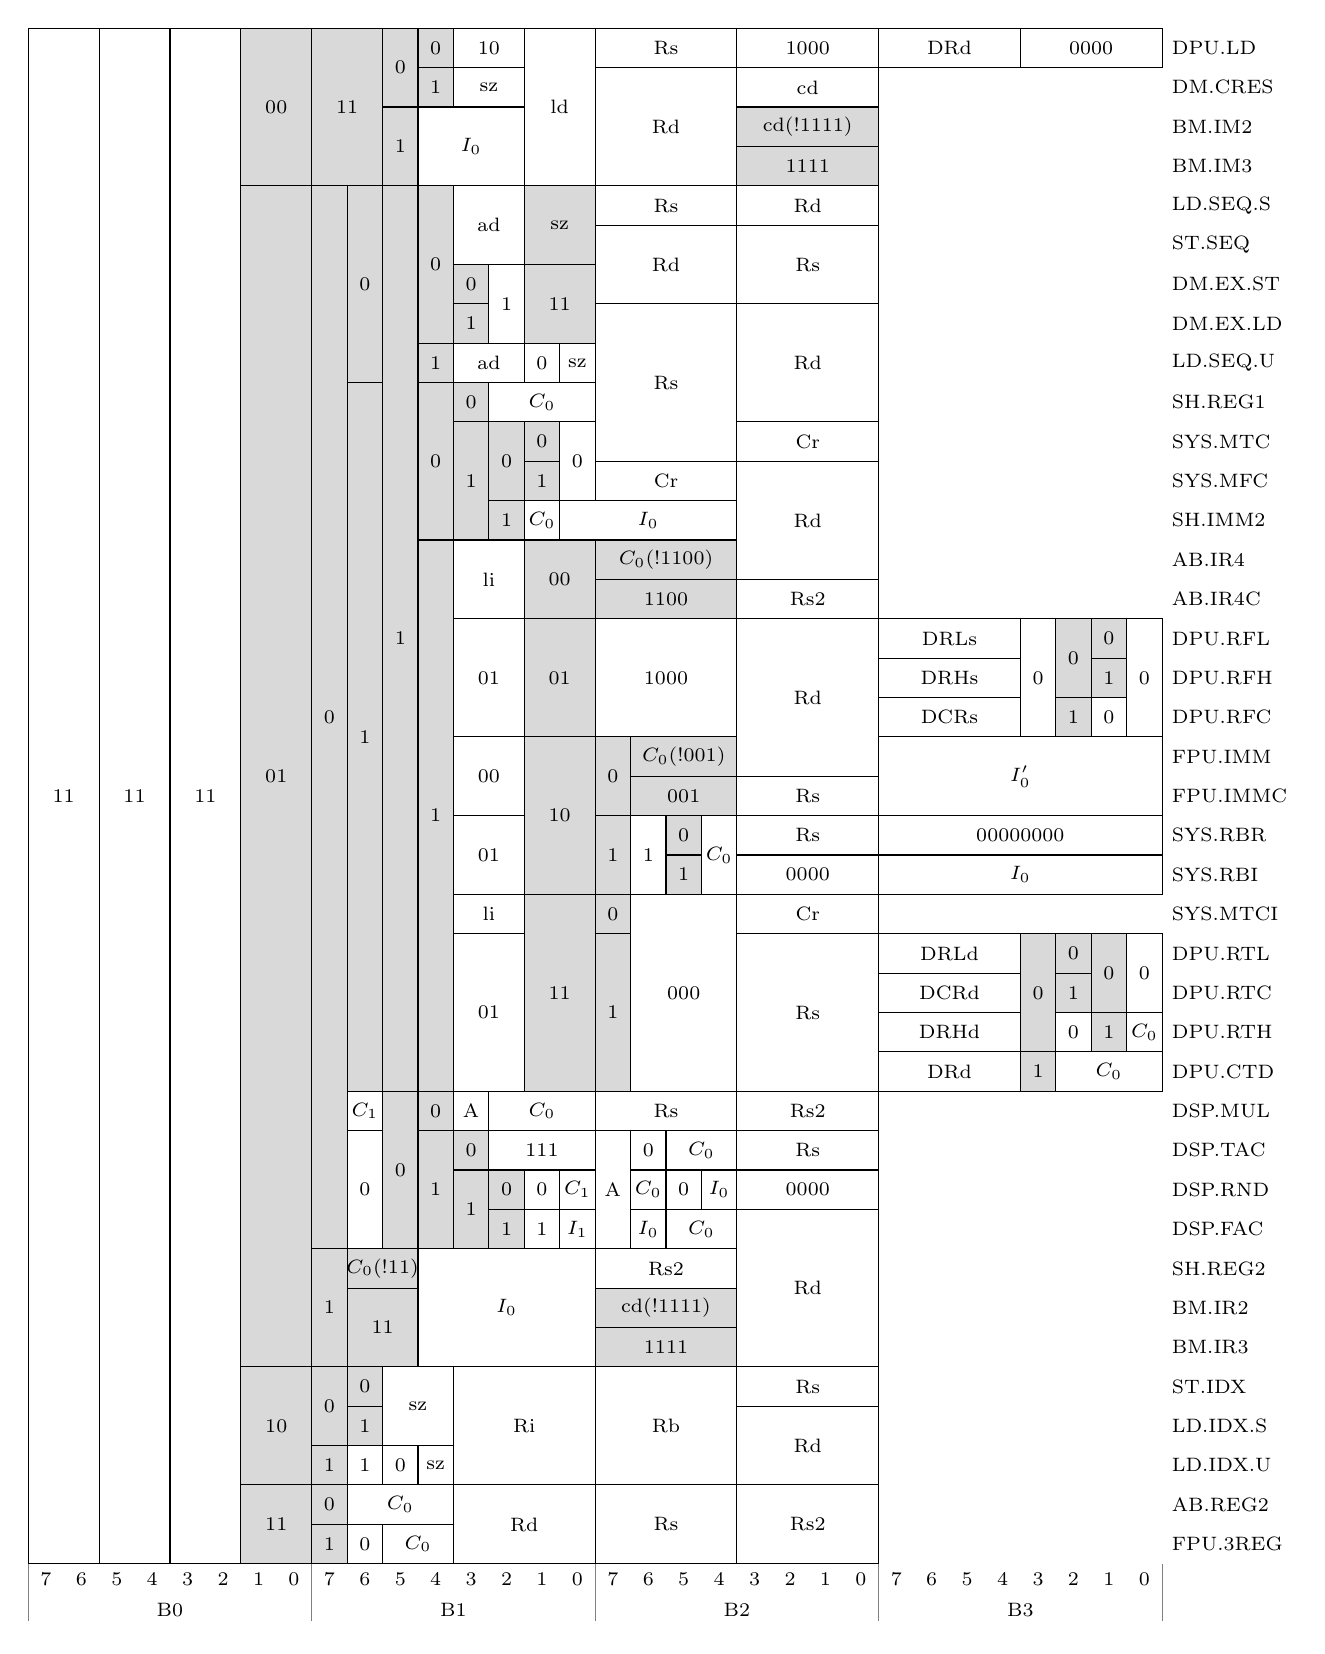
\begin{tikzpicture}[xscale=0.45,yscale=0.25]
\foreach \x in {0, 1, ..., 31}
    \draw (\x + 0.5, 1) node[anchor=north] {\scriptsize \pgfmathparse{int(7 - mod(\x, 8))}\pgfmathresult};
\draw (4, -0.5) node[anchor=north] {\scriptsize B0};
\draw (12, -0.5) node[anchor=north] {\scriptsize B1};
\draw (20, -0.5) node[anchor=north] {\scriptsize B2};
\draw (28, -0.5) node[anchor=north] {\scriptsize B3};
\foreach \x in {0, 8, 16, 24, 32}
    \draw[gray] (\x, -1.9) -- (\x, 1);

% Encoding
% B0(7)
\draw (0, \fputhreeregp * 2 + 1) rectangle (2, \dpuldp * 2 + 3) node[pos=.5] {\scriptsize 11};
% B0(5)
\draw (2, \fputhreeregp * 2 + 1) rectangle (4, \dpuldp * 2 + 3) node[pos=.5] {\scriptsize 11};
% B0(3)
\draw (4, \fputhreeregp * 2 + 1) rectangle (6, \dpuldp * 2 + 3) node[pos=.5] {\scriptsize 11};
% B0(1)
\fill[black!15] (6, \bmimfourp * 2 + 1) rectangle (8, \dpuldp * 2 + 3);
\draw (6, \bmimfourp * 2 + 1) rectangle (8, \dpuldp * 2 + 3) node[pos=.5] {\scriptsize 00};
\fill[black!15] (6, \bmirthreep * 2 + 1) rectangle (8, \ldseqsp * 2 + 3);
\draw (6, \bmirthreep * 2 + 1) rectangle (8, \ldseqsp * 2 + 3) node[pos=.5] {\scriptsize 01};
\fill[black!15] (6, \ldidxup * 2 + 1) rectangle (8, \stidxp * 2 + 3);
\draw (6, \ldidxup * 2 + 1) rectangle (8, \stidxp * 2 + 3) node[pos=.5] {\scriptsize 10};
\fill[black!15] (6, \fputhreeregp * 2 + 1) rectangle (8, \iaabregtwop * 2 + 3);
\draw (6, \fputhreeregp * 2 + 1) rectangle (8, \iaabregtwop * 2 + 3) node[pos=.5] {\scriptsize 11};

% B1(7)
\fill[black!15] (8, \bmimfourp * 2 + 1) rectangle (10, \dpuldp * 2 + 3);
\draw (8, \bmimfourp * 2 + 1) rectangle (10, \dpuldp * 2 + 3) node[pos=.5] {\scriptsize 11};
\fill[black!15] (8, \dspfacp * 2 + 1) rectangle (9, \ldseqsp * 2 + 3);
\draw (8, \dspfacp * 2 + 1) rectangle (9, \ldseqsp * 2 + 3) node[pos=.5] {\scriptsize 0};
\fill[black!15] (8, \bmirthreep * 2 + 1) rectangle (9, \iashregtwop * 2 + 3);
\draw (8, \bmirthreep * 2 + 1) rectangle (9, \iashregtwop * 2 + 3) node[pos=.5] {\scriptsize 1};
\fill[black!15] (8, \ldidxsp * 2 + 1) rectangle (9, \stidxp * 2 + 3);
\draw (8, \ldidxsp * 2 + 1) rectangle (9, \stidxp * 2 + 3) node[pos=.5] {\scriptsize 0};
\fill[black!15] (8, \ldidxup * 2 + 1) rectangle (9, \ldidxup * 2 + 3);
\draw (8, \ldidxup * 2 + 1) rectangle (9, \ldidxup * 2 + 3) node[pos=.5] {\scriptsize 1};
\fill[black!15] (8, \iaabregtwop * 2 + 1) rectangle (9, \iaabregtwop * 2 + 3);
\draw (8, \iaabregtwop * 2 + 1) rectangle (9, \iaabregtwop * 2 + 3) node[pos=.5] {\scriptsize 0};
\fill[black!15] (8, \fputhreeregp * 2 + 1) rectangle (9, \fputhreeregp * 2 + 3);
\draw (8, \fputhreeregp * 2 + 1) rectangle (9, \fputhreeregp * 2 + 3) node[pos=.5] {\scriptsize 1};

% B1(6)
\fill[black!15] (9, \lssequp * 2 + 1) rectangle (10, \ldseqsp * 2 + 3);
\draw (9, \lssequp * 2 + 1) rectangle (10, \ldseqsp * 2 + 3) node[pos=.5] {\scriptsize 0};
\fill[black!15] (9, \dpuctdp * 2 + 1) rectangle (10, \iashregonep * 2 + 3);
\draw (9, \dpuctdp * 2 + 1) rectangle (10, \iashregonep * 2 + 3) node[pos=.5] {\scriptsize 1};
\draw (9, \dspmulp * 2 + 1) rectangle (10, \dspmulp * 2 + 3) node[pos=.5] {\scriptsize $C_1$};
\draw (9, \dspfacp * 2 + 1) rectangle (10, \dsptacp * 2 + 3) node[pos=.5] {\scriptsize 0};
\fill[black!15] (9, \iashregtwop * 2 + 1) rectangle (11, \iashregtwop * 2 + 3);
\draw (9, \iashregtwop * 2 + 1) rectangle (11, \iashregtwop * 2 + 3) node[pos=.5] {\scriptsize $C_0$(!11)};
\fill[black!15] (9, \bmirthreep * 2 + 1) rectangle (11, \bmirtwop * 2 + 3);
\draw (9, \bmirthreep * 2 + 1) rectangle (11, \bmirtwop * 2 + 3) node[pos=.5] {\scriptsize 11};
\fill[black!15] (9, \stidxp * 2 + 1) rectangle (10, \stidxp * 2 + 3);
\draw (9, \stidxp * 2 + 1) rectangle (10, \stidxp * 2 + 3) node[pos=.5] {\scriptsize 0};
\fill[black!15] (9, \ldidxsp * 2 + 1) rectangle (10, \ldidxsp * 2 + 3);
\draw (9, \ldidxsp * 2 + 1) rectangle (10, \ldidxsp * 2 + 3) node[pos=.5] {\scriptsize 1};
\draw (9, \ldidxup * 2 + 1) rectangle (10, \ldidxup * 2 + 3) node[pos=.5] {\scriptsize 1};
\draw (9, \iaabregtwop * 2 + 1) rectangle (12, \iaabregtwop * 2 + 3) node[pos=.5] {\scriptsize $C_0$};
\draw (9, \fputhreeregp * 2 + 1) rectangle (10, \fputhreeregp * 2 + 3) node[pos=.5] {\scriptsize 0};

% B1(5)
\fill[black!15] (10, \dmcresp * 2 + 1) rectangle (11, \dpuldp * 2 + 3);
\draw (10, \dmcresp * 2 + 1) rectangle (11, \dpuldp * 2 + 3) node[pos=.5] {\scriptsize 0};
\fill[black!15] (10, \bmimfourp * 2 + 1) rectangle (11, \bmimthreep * 2 + 3);
\draw (10, \bmimfourp * 2 + 1) rectangle (11, \bmimthreep * 2 + 3) node[pos=.5] {\scriptsize 1};
\fill[black!15] (10, \dpuctdp * 2 + 1) rectangle (11, \ldseqsp * 2 + 3);
\draw (10, \dpuctdp * 2 + 1) rectangle (11, \ldseqsp * 2 + 3) node[pos=.5] {\scriptsize 1};
\fill[black!15] (10, \dspfacp * 2 + 1) rectangle (11, \dspmulp * 2 + 3);
\draw (10, \dspfacp * 2 + 1) rectangle (11, \dspmulp * 2 + 3) node[pos=.5] {\scriptsize 0};
\draw (10, \ldidxsp * 2 + 1) rectangle (12, \stidxp * 2 + 3) node[pos=.5] {\scriptsize sz};
\draw (10, \ldidxup * 2 + 1) rectangle (11, \ldidxup * 2 + 3) node[pos=.5] {\scriptsize 0};
\draw (10, \fputhreeregp * 2 + 1) rectangle (12, \fputhreeregp * 2 + 3) node[pos=.5] {\scriptsize $C_0$};

% B1(4)
\fill[black!15] (11, \dpuldp * 2 + 1) rectangle (12, \dpuldp * 2 + 3);
\draw (11, \dpuldp * 2 + 1) rectangle (12, \dpuldp * 2 + 3) node[pos=.5] {\scriptsize 0};
\fill[black!15] (11, \dmcresp * 2 + 1) rectangle (12, \dmcresp * 2 + 3);
\draw (11, \dmcresp * 2 + 1) rectangle (12, \dmcresp * 2 + 3) node[pos=.5] {\scriptsize 1};
\draw (11, \bmimfourp * 2 + 1) rectangle (14, \bmimthreep * 2 + 3) node[pos=.5] {\scriptsize $I_0$};
\fill[black!15] (11, \dmexldp * 2 + 1) rectangle (12, \ldseqsp * 2 + 3);
\draw (11, \dmexldp * 2 + 1) rectangle (12, \ldseqsp * 2 + 3) node[pos=.5] {\scriptsize 0};
\fill[black!15] (11, \lssequp * 2 + 1) rectangle (12, \lssequp * 2 + 3);
\draw (11, \lssequp * 2 + 1) rectangle (12, \lssequp * 2 + 3) node[pos=.5] {\scriptsize 1};
\fill[black!15] (11, \iashimmtwop * 2 + 1) rectangle (12, \iashregonep * 2 + 3);
\draw (11, \iashimmtwop * 2 + 1) rectangle (12, \iashregonep * 2 + 3) node[pos=.5] {\scriptsize 0};
\fill[black!15] (11, \dpuctdp * 2 + 1) rectangle (12, \iaabirfourp * 2 + 3);
\draw (11, \dpuctdp * 2 + 1) rectangle (12, \iaabirfourp * 2 + 3) node[pos=.5] {\scriptsize 1};
\fill[black!15] (11, \dspmulp * 2 + 1) rectangle (12, \dspmulp * 2 + 3);
\draw (11, \dspmulp * 2 + 1) rectangle (12, \dspmulp * 2 + 3) node[pos=.5] {\scriptsize 0};
\fill[black!15] (11, \dspfacp * 2 + 1) rectangle (12, \dsptacp * 2 + 3);
\draw (11, \dspfacp * 2 + 1) rectangle (12, \dsptacp * 2 + 3) node[pos=.5] {\scriptsize 1};
\draw (11, \bmirthreep * 2 + 1) rectangle (16, \iashregtwop * 2 + 3) node[pos=.5] {\scriptsize $I_0$};
\draw (11, \ldidxup * 2 + 1) rectangle (12, \ldidxup * 2 + 3) node[pos=.5] {\scriptsize sz};

% B1(3)
\draw (12, \dpuldp * 2 + 1) rectangle (14, \dpuldp * 2 + 3) node[pos=.5] {\scriptsize 10};
\draw (12, \dmcresp * 2 + 1) rectangle (14, \dmcresp * 2 + 3) node[pos=.5] {\scriptsize sz};
\draw (12, \stseqp * 2 + 1) rectangle (14, \ldseqsp * 2 + 3) node[pos=.5] {\scriptsize ad};
\fill[black!15] (12, \dmexstp * 2 + 1) rectangle (13, \dmexstp * 2 + 3);
\draw (12, \dmexstp * 2 + 1) rectangle (13, \dmexstp * 2 + 3) node[pos=.5] {\scriptsize 0};
\fill[black!15] (12, \dmexldp * 2 + 1) rectangle (13, \dmexldp * 2 + 3);
\draw (12, \dmexldp * 2 + 1) rectangle (13, \dmexldp * 2 + 3) node[pos=.5] {\scriptsize 1};
\draw (12, \lssequp * 2 + 1) rectangle (14, \lssequp * 2 + 3) node[pos=.5] {\scriptsize ad};
\fill[black!15] (12, \iashregonep * 2 + 1) rectangle (13, \iashregonep * 2 + 3);
\draw (12, \iashregonep * 2 + 1) rectangle (13, \iashregonep * 2 + 3) node[pos=.5] {\scriptsize 0};
\fill[black!15] (12, \iashimmtwop * 2 + 1) rectangle (13, \sysmtcp * 2 + 3);
\draw (12, \iashimmtwop * 2 + 1) rectangle (13, \sysmtcp * 2 + 3) node[pos=.5] {\scriptsize 1};
\draw (12, \iaabirfourcp * 2 + 1) rectangle (14, \iaabirfourp * 2 + 3) node[pos=.5] {\scriptsize li};
\draw (12, \dpurfcp * 2 + 1) rectangle (14, \dpurflp * 2 + 3) node[pos=.5] {\scriptsize 01};
\draw (12, \fpuimmcp * 2 + 1) rectangle (14, \fpuimmp * 2 + 3) node[pos=.5] {\scriptsize 00};
\draw (12, \sysrbip * 2 + 1) rectangle (14, \sysrbrp * 2 + 3) node[pos=.5] {\scriptsize 01};
\draw (12, \sysmtcip * 2 + 1) rectangle (14, \sysmtcip * 2 + 3) node[pos=.5] {\scriptsize li};
\draw (12, \dpuctdp * 2 + 1) rectangle (14, \dpurtlp * 2 + 3) node[pos=.5] {\scriptsize 01};
\draw (12, \dspmulp * 2 + 1) rectangle (13, \dspmulp * 2 + 3) node[pos=.5] {\scriptsize A};
\fill[black!15] (12, \dsptacp * 2 + 1) rectangle (13, \dsptacp * 2 + 3);
\draw (12, \dsptacp * 2 + 1) rectangle (13, \dsptacp * 2 + 3) node[pos=.5] {\scriptsize 0};
\fill[black!15] (12, \dspfacp * 2 + 1) rectangle (13, \dsprndp * 2 + 3);
\draw (12, \dspfacp * 2 + 1) rectangle (13, \dsprndp * 2 + 3) node[pos=.5] {\scriptsize 1};
\draw (12, \ldidxup * 2 + 1) rectangle (16, \stidxp * 2 + 3) node[pos=.5] {\scriptsize Ri};
\draw (12, \fputhreeregp * 2 + 1) rectangle (16, \iaabregtwop * 2 + 3) node[pos=.5] {\scriptsize Rd};

% B1(2)
\draw (13, \dmexldp * 2 + 1) rectangle (14, \dmexstp * 2 + 3) node[pos=.5] {\scriptsize 1};
\draw (13, \iashregonep * 2 + 1) rectangle (16, \iashregonep * 2 + 3) node[pos=.5] {\scriptsize $C_0$};
\fill[black!15] (13, \sysmfcp * 2 + 1) rectangle (14, \sysmtcp * 2 + 3);
\draw (13, \sysmfcp * 2 + 1) rectangle (14, \sysmtcp * 2 + 3) node[pos=.5] {\scriptsize 0};
\fill[black!15] (13, \iashimmtwop * 2 + 1) rectangle (14, \iashimmtwop * 2 + 3);
\draw (13, \iashimmtwop * 2 + 1) rectangle (14, \iashimmtwop * 2 + 3) node[pos=.5] {\scriptsize 1};
\draw (13, \dspmulp * 2 + 1) rectangle (16, \dspmulp * 2 + 3) node[pos=.5] {\scriptsize $C_0$};
\draw (13, \dsptacp * 2 + 1) rectangle (16, \dsptacp * 2 + 3) node[pos=.5] {\scriptsize 111};
\fill[black!15] (13, \dsprndp * 2 + 1) rectangle (14, \dsprndp * 2 + 3);
\draw (13, \dsprndp * 2 + 1) rectangle (14, \dsprndp * 2 + 3) node[pos=.5] {\scriptsize 0};
\fill[black!15] (13, \dspfacp * 2 + 1) rectangle (14, \dspfacp * 2 + 3);
\draw (13, \dspfacp * 2 + 1) rectangle (14, \dspfacp * 2 + 3) node[pos=.5] {\scriptsize 1};

% B1(1)
\fill[black!15] (14, \dpuctdp * 2 + 1) rectangle (16, \sysmtcip * 2 + 3);
\draw (14, \bmimfourp * 2 + 1) rectangle (16, \dpuldp * 2 + 3) node[pos=.5] {\scriptsize ld};
\fill[black!15] (14, \stseqp * 2 + 1) rectangle (16, \ldseqsp * 2 + 3);
\draw (14, \stseqp * 2 + 1) rectangle (16, \ldseqsp * 2 + 3) node[pos=.5] {\scriptsize sz};
\fill[black!15] (14, \dmexldp * 2 + 1) rectangle (16, \dmexstp * 2 + 3);
\draw (14, \dmexldp * 2 + 1) rectangle (16, \dmexstp * 2 + 3) node[pos=.5] {\scriptsize 11};
\draw (14, \lssequp * 2 + 1) rectangle (15, \lssequp * 2 + 3) node[pos=.5] {\scriptsize 0};
\fill[black!15] (14, \sysmtcp * 2 + 1) rectangle (15, \sysmtcp * 2 + 3);
\draw (14, \sysmtcp * 2 + 1) rectangle (15, \sysmtcp * 2 + 3) node[pos=.5] {\scriptsize 0};
\fill[black!15] (14, \sysmfcp * 2 + 1) rectangle (15, \sysmfcp * 2 + 3);
\draw (14, \sysmfcp * 2 + 1) rectangle (15, \sysmfcp * 2 + 3) node[pos=.5] {\scriptsize 1};
\draw (14, \iashimmtwop * 2 + 1) rectangle (15, \iashimmtwop * 2 + 3) node[pos=.5] {\scriptsize $C_0$};
\fill[black!15] (14, \iaabirfourcp * 2 + 1) rectangle (16, \iaabirfourp * 2 + 3);
\draw (14, \iaabirfourcp * 2 + 1) rectangle (16, \iaabirfourp * 2 + 3) node[pos=.5] {\scriptsize 00};
\fill[black!15] (14, \dpurfcp * 2 + 1) rectangle (16, \dpurflp * 2 + 3);
\draw (14, \dpurfcp * 2 + 1) rectangle (16, \dpurflp * 2 + 3) node[pos=.5] {\scriptsize 01};
\fill[black!15] (14, \sysrbip * 2 + 1) rectangle (16, \fpuimmp * 2 + 3);
\draw (14, \sysrbip * 2 + 1) rectangle (16, \fpuimmp * 2 + 3) node[pos=.5] {\scriptsize 10};
\draw (14, \dpuctdp * 2 + 1) rectangle (16, \sysmtcip * 2 + 3) node[pos=.5] {\scriptsize 11};
\draw (14, \dsprndp * 2 + 1) rectangle (15, \dsprndp * 2 + 3) node[pos=.5] {\scriptsize 0};
\draw (14, \dspfacp * 2 + 1) rectangle (15, \dspfacp * 2 + 3) node[pos=.5] {\scriptsize 1};

% B1(0)
\draw (15, \lssequp * 2 + 1) rectangle (16, \lssequp * 2 + 3) node[pos=.5] {\scriptsize sz};
\draw (15, \sysmfcp * 2 + 1) rectangle (16, \sysmtcp * 2 + 3) node[pos=.5] {\scriptsize 0};
\draw (15, \iashimmtwop * 2 + 1) rectangle (20, \iashimmtwop * 2 + 3) node[pos=.5] {\scriptsize $I_0$};
\draw (15, \dsprndp * 2 + 1) rectangle (16, \dsprndp * 2 + 3) node[pos=.5] {\scriptsize $C_1$};
\draw (15, \dspfacp * 2 + 1) rectangle (16, \dspfacp * 2 + 3) node[pos=.5] {\scriptsize $I_1$};

% B2(7)
\draw (16, \dpuldp * 2 + 1) rectangle (20, \dpuldp * 2 + 3) node[pos=.5] {\scriptsize Rs};
\draw (16, \bmimfourp * 2 + 1) rectangle (20, \dmcresp * 2 + 3) node[pos=.5] {\scriptsize Rd};
\draw (16, \ldseqsp * 2 + 1) rectangle (20, \ldseqsp * 2 + 3) node[pos=.5] {\scriptsize Rs};
\draw (16, \dmexstp * 2 + 1) rectangle (20, \stseqp * 2 + 3) node[pos=.5] {\scriptsize Rd};
\draw (16, \sysmtcp * 2 + 1) rectangle (20, \dmexldp * 2 + 3) node[pos=.5] {\scriptsize Rs};
\draw (16, \sysmfcp * 2 + 1) rectangle (20, \sysmfcp * 2 + 3) node[pos=.5] {\scriptsize Cr};
\fill[black!15] (16, \iaabirfourp * 2 + 1) rectangle (20, \iaabirfourp * 2 + 3);
\draw (16, \iaabirfourp * 2 + 1) rectangle (20, \iaabirfourp * 2 + 3) node[pos=.5] {\scriptsize $C_0$(!1100)};
\fill[black!15] (16, \iaabirfourcp * 2 + 1) rectangle (20, \iaabirfourcp * 2 + 3);
\draw (16, \iaabirfourcp * 2 + 1) rectangle (20, \iaabirfourcp * 2 + 3) node[pos=.5] {\scriptsize 1100};
\draw (16, \dpurfcp * 2 + 1) rectangle (20, \dpurflp * 2 + 3) node[pos=.5] {\scriptsize 1000};
\fill[black!15] (16, \fpuimmcp * 2 + 1) rectangle (17, \fpuimmp * 2 + 3);
\draw (16, \fpuimmcp * 2 + 1) rectangle (17, \fpuimmp * 2 + 3) node[pos=.5] {\scriptsize 0};
\fill[black!15] (16, \sysrbip * 2 + 1) rectangle (17, \sysrbrp * 2 + 3);
\draw (16, \sysrbip * 2 + 1) rectangle (17, \sysrbrp * 2 + 3) node[pos=.5] {\scriptsize 1};
\fill[black!15] (16, \sysmtcip * 2 + 1) rectangle (17, \sysmtcip * 2 + 3);
\draw (16, \sysmtcip * 2 + 1) rectangle (17, \sysmtcip * 2 + 3) node[pos=.5] {\scriptsize 0};
\fill[black!15] (16, \dpuctdp * 2 + 1) rectangle (17, \dpurtlp * 2 + 3);
\draw (16, \dpuctdp * 2 + 1) rectangle (17, \dpurtlp * 2 + 3) node[pos=.5] {\scriptsize 1};
\draw (16, \dspmulp * 2 + 1) rectangle (20, \dspmulp * 2 + 3) node[pos=.5] {\scriptsize Rs};
\draw (16, \dspfacp * 2 + 1) rectangle (17, \dsptacp * 2 + 3) node[pos=.5] {\scriptsize A};
\draw (16, \iashregtwop * 2 + 1) rectangle (20, \iashregtwop * 2 + 3) node[pos=.5] {\scriptsize Rs2};
\fill[black!15] (16, \bmirtwop * 2 + 1) rectangle (20, \bmirtwop * 2 + 3);
\draw (16, \bmirtwop * 2 + 1) rectangle (20, \bmirtwop * 2 + 3) node[pos=.5] {\scriptsize cd(!1111)};
\fill[black!15] (16, \bmirthreep * 2 + 1) rectangle (20, \bmirthreep * 2 + 3);
\draw (16, \bmirthreep * 2 + 1) rectangle (20, \bmirthreep * 2 + 3) node[pos=.5] {\scriptsize 1111};
\draw (16, \ldidxup * 2 + 1) rectangle (20, \stidxp * 2 + 3) node[pos=.5] {\scriptsize Rb};
\draw (16, \fputhreeregp * 2 + 1) rectangle (20, \iaabregtwop * 2 + 3) node[pos=.5] {\scriptsize Rs};

% B2(6)
\fill[black!15] (17, \fpuimmp * 2 + 1) rectangle (20, \fpuimmp * 2 + 3);
\draw (17, \fpuimmp * 2 + 1) rectangle (20, \fpuimmp * 2 + 3) node[pos=.5] {\scriptsize $C_0$(!001)};
\fill[black!15] (17, \fpuimmcp * 2 + 1) rectangle (20, \fpuimmcp * 2 + 3);
\draw (17, \fpuimmcp * 2 + 1) rectangle (20, \fpuimmcp * 2 + 3) node[pos=.5] {\scriptsize 001};
\draw (17, \sysrbip * 2 + 1) rectangle (18, \sysrbrp * 2 + 3) node[pos=.5] {\scriptsize 1};
\draw (17, \dpuctdp * 2 + 1) rectangle (20, \sysmtcip * 2 + 3) node[pos=.5] {\scriptsize 000};
\draw (17, \dsptacp * 2 + 1) rectangle (18, \dsptacp * 2 + 3) node[pos=.5] {\scriptsize 0};
\draw (17, \dsprndp * 2 + 1) rectangle (18, \dsprndp * 2 + 3) node[pos=.5] {\scriptsize $C_0$};
\draw (17, \dspfacp * 2 + 1) rectangle (18, \dspfacp * 2 + 3) node[pos=.5] {\scriptsize $I_0$};

% B2(5)
\fill[black!15] (18, \sysrbrp * 2 + 1) rectangle (19, \sysrbrp * 2 + 3);
\draw (18, \sysrbrp * 2 + 1) rectangle (19, \sysrbrp * 2 + 3) node[pos=.5] {\scriptsize 0};
\fill[black!15] (18, \sysrbip * 2 + 1) rectangle (19, \sysrbip * 2 + 3);
\draw (18, \sysrbip * 2 + 1) rectangle (19, \sysrbip * 2 + 3) node[pos=.5] {\scriptsize 1};
\draw (18, \dsptacp * 2 + 1) rectangle (20, \dsptacp * 2 + 3) node[pos=.5] {\scriptsize $C_0$};
\draw (18, \dsprndp * 2 + 1) rectangle (19, \dsprndp * 2 + 3) node[pos=.5] {\scriptsize 0};
\draw (18, \dspfacp * 2 + 1) rectangle (20, \dspfacp * 2 + 3) node[pos=.5] {\scriptsize $C_0$};

% B2(4)
\draw (19, \sysrbip * 2 + 1) rectangle (20, \sysrbrp * 2 + 3) node[pos=.5] {\scriptsize $C_0$};
\draw (19, \dsprndp * 2 + 1) rectangle (20, \dsprndp * 2 + 3) node[pos=.5] {\scriptsize $I_0$};

% B2(3)
\draw (20, \dpuldp * 2 + 1) rectangle (24, \dpuldp * 2 + 3) node[pos=.5] {\scriptsize 1000};
\draw (20, \dmcresp * 2 + 1) rectangle (24, \dmcresp * 2 + 3) node[pos=.5] {\scriptsize cd};
\fill[black!15] (20, \bmimthreep * 2 + 1) rectangle (24, \bmimthreep * 2 + 3);
\draw (20, \bmimthreep * 2 + 1) rectangle (24, \bmimthreep * 2 + 3) node[pos=.5] {\scriptsize cd(!1111)};
\fill[black!15] (20, \bmimfourp * 2 + 1) rectangle (24, \bmimfourp * 2 + 3);
\draw (20, \bmimfourp * 2 + 1) rectangle (24, \bmimfourp * 2 + 3) node[pos=.5] {\scriptsize 1111};
\draw (20, \ldseqsp * 2 + 1) rectangle (24, \ldseqsp * 2 + 3) node[pos=.5] {\scriptsize Rd};
\draw (20, \dmexstp * 2 + 1) rectangle (24, \stseqp * 2 + 3) node[pos=.5] {\scriptsize Rs};
\draw (20, \iashregonep * 2 + 1) rectangle (24, \dmexldp * 2 + 3) node[pos=.5] {\scriptsize Rd};
\draw (20, \sysmtcp * 2 + 1) rectangle (24, \sysmtcp * 2 + 3) node[pos=.5] {\scriptsize Cr};
\draw (20, \iaabirfourp * 2 + 1) rectangle (24, \sysmfcp * 2 + 3) node[pos=.5] {\scriptsize Rd};
\draw (20, \iaabirfourcp * 2 + 1) rectangle (24, \iaabirfourcp * 2 + 3) node[pos=.5] {\scriptsize Rs2};
\draw (20, \fpuimmp * 2 + 1) rectangle (24, \dpurflp * 2 + 3) node[pos=.5] {\scriptsize Rd};
\draw (20, \fpuimmcp * 2 + 1) rectangle (24, \fpuimmcp * 2 + 3) node[pos=.5] {\scriptsize Rs};
\draw (20, \sysrbrp * 2 + 1) rectangle (24, \sysrbrp * 2 + 3) node[pos=.5] {\scriptsize Rs};
\draw (20, \sysrbip * 2 + 1) rectangle (24, \sysrbip * 2 + 3) node[pos=.5] {\scriptsize 0000};
\draw (20, \sysmtcip * 2 + 1) rectangle (24, \sysmtcip * 2 + 3) node[pos=.5] {\scriptsize Cr};
\draw (20, \dpuctdp * 2 + 1) rectangle (24, \dpurtlp * 2 + 3) node[pos=.5] {\scriptsize Rs};
\draw (20, \dspmulp * 2 + 1) rectangle (24, \dspmulp * 2 + 3) node[pos=.5] {\scriptsize Rs2};
\draw (20, \dsptacp * 2 + 1) rectangle (24, \dsptacp * 2 + 3) node[pos=.5] {\scriptsize Rs};
\draw (20, \dsprndp * 2 + 1) rectangle (24, \dsprndp * 2 + 3) node[pos=.5] {\scriptsize 0000};
\draw (20, \bmirthreep * 2 + 1) rectangle (24, \dspfacp * 2 + 3) node[pos=.5] {\scriptsize Rd};
\draw (20, \stidxp * 2 + 1) rectangle (24, \stidxp * 2 + 3) node[pos=.5] {\scriptsize Rs};
\draw (20, \ldidxup * 2 + 1) rectangle (24, \ldidxsp * 2 + 3) node[pos=.5] {\scriptsize Rd};
\draw (20, \fputhreeregp * 2 + 1) rectangle (24, \iaabregtwop * 2 + 3) node[pos=.5] {\scriptsize Rs2};

% B3(7)
\draw (24, \dpuldp * 2 + 1) rectangle (28, \dpuldp * 2 + 3) node[pos=.5] {\scriptsize DRd};
\draw (24, \dpurflp * 2 + 1) rectangle (28, \dpurflp * 2 + 3) node[pos=.5] {\scriptsize DRLs};
\draw (24, \dpurfhp * 2 + 1) rectangle (28, \dpurfhp * 2 + 3) node[pos=.5] {\scriptsize DRHs};
\draw (24, \dpurfcp * 2 + 1) rectangle (28, \dpurfcp * 2 + 3) node[pos=.5] {\scriptsize DCRs};
\draw (24, \fpuimmcp * 2 + 1) rectangle (32, \fpuimmp * 2 + 3) node[pos=.5] {\scriptsize $I_0'$};
\draw (24, \sysrbrp * 2 + 1) rectangle (32, \sysrbrp * 2 + 3) node[pos=.5] {\scriptsize 00000000};
\draw (24, \sysrbip * 2 + 1) rectangle (32, \sysrbip * 2 + 3) node[pos=.5] {\scriptsize $I_0$};
\draw (24, \dpurtlp * 2 + 1) rectangle (28, \dpurtlp * 2 + 3) node[pos=.5] {\scriptsize DRLd};
\draw (24, \dpurtcp * 2 + 1) rectangle (28, \dpurtcp * 2 + 3) node[pos=.5] {\scriptsize DCRd};
\draw (24, \dpurthp * 2 + 1) rectangle (28, \dpurthp * 2 + 3) node[pos=.5] {\scriptsize DRHd};
\draw (24, \dpuctdp * 2 + 1) rectangle (28, \dpuctdp * 2 + 3) node[pos=.5] {\scriptsize DRd};

% B3(3)
\draw (28, \dpuldp * 2 + 1) rectangle (32, \dpuldp * 2 + 3) node[pos=.5] {\scriptsize 0000};
\draw (28, \dpurfcp * 2 + 1) rectangle (29, \dpurflp * 2 + 3) node[pos=.5] {\scriptsize 0};
\fill[black!15] (28, \dpurthp * 2 + 1) rectangle (29, \dpurtlp * 2 + 3);
\draw (28, \dpurthp * 2 + 1) rectangle (29, \dpurtlp * 2 + 3) node[pos=.5] {\scriptsize 0};
\fill[black!15] (28, \dpuctdp * 2 + 1) rectangle (29, \dpuctdp * 2 + 3);
\draw (28, \dpuctdp * 2 + 1) rectangle (29, \dpuctdp * 2 + 3) node[pos=.5] {\scriptsize 1};

% B3(2)
\fill[black!15] (29, \dpurfhp * 2 + 1) rectangle (30, \dpurflp * 2 + 3);
\draw (29, \dpurfhp * 2 + 1) rectangle (30, \dpurflp * 2 + 3) node[pos=.5] {\scriptsize 0};
\fill[black!15] (29, \dpurfcp * 2 + 1) rectangle (30, \dpurfcp * 2 + 3);
\draw (29, \dpurfcp * 2 + 1) rectangle (30, \dpurfcp * 2 + 3) node[pos=.5] {\scriptsize 1};
\fill[black!15] (29, \dpurtlp * 2 + 1) rectangle (30, \dpurtlp * 2 + 3);
\draw (29, \dpurtlp * 2 + 1) rectangle (30, \dpurtlp * 2 + 3) node[pos=.5] {\scriptsize 0};
\fill[black!15] (29, \dpurtcp * 2 + 1) rectangle (30, \dpurtcp * 2 + 3);
\draw (29, \dpurtcp * 2 + 1) rectangle (30, \dpurtcp * 2 + 3) node[pos=.5] {\scriptsize 1};
\draw (29, \dpurthp * 2 + 1) rectangle (30, \dpurthp * 2 + 3) node[pos=.5] {\scriptsize 0};
\draw (29, \dpuctdp * 2 + 1) rectangle (32, \dpuctdp * 2 + 3) node[pos=.5] {\scriptsize $C_0$};

% B3(1)
\fill[black!15] (30, \dpurflp * 2 + 1) rectangle (31, \dpurflp * 2 + 3);
\draw (30, \dpurflp * 2 + 1) rectangle (31, \dpurflp * 2 + 3) node[pos=.5] {\scriptsize 0};
\fill[black!15] (30, \dpurfhp * 2 + 1) rectangle (31, \dpurfhp * 2 + 3);
\draw (30, \dpurfhp * 2 + 1) rectangle (31, \dpurfhp * 2 + 3) node[pos=.5] {\scriptsize 1};
\draw (30, \dpurfcp * 2 + 1) rectangle (31, \dpurfcp * 2 + 3) node[pos=.5] {\scriptsize 0};
\fill[black!15] (30, \dpurtcp * 2 + 1) rectangle (31, \dpurtlp * 2 + 3);
\draw (30, \dpurtcp * 2 + 1) rectangle (31, \dpurtlp * 2 + 3) node[pos=.5] {\scriptsize 0};
\fill[black!15] (30, \dpurthp * 2 + 1) rectangle (31, \dpurthp * 2 + 3);
\draw (30, \dpurthp * 2 + 1) rectangle (31, \dpurthp * 2 + 3) node[pos=.5] {\scriptsize 1};

% B3(0)
\draw (31, \dpurfcp * 2 + 1) rectangle (32, \dpurflp * 2 + 3) node[pos=.5] {\scriptsize 0};
\draw (31, \dpurtcp * 2 + 1) rectangle (32, \dpurtlp * 2 + 3) node[pos=.5] {\scriptsize 0};
\draw (31, \dpurthp * 2 + 1) rectangle (32, \dpurthp * 2 + 3) node[pos=.5] {\scriptsize $C_0$};

% Group names
\draw (32, \dpuldp * 2 + 2) node[anchor=west] {\scriptsize DPU.LD};
\draw (32, \dmcresp * 2 + 2) node[anchor=west] {\scriptsize DM.CRES};
\draw (32, \bmimthreep * 2 + 2) node[anchor=west] {\scriptsize BM.IM2};
\draw (32, \bmimfourp * 2 + 2) node[anchor=west] {\scriptsize BM.IM3};
\draw (32, \ldseqsp * 2 + 2) node[anchor=west] {\scriptsize LD.SEQ.S};
\draw (32, \stseqp * 2 + 2) node[anchor=west] {\scriptsize ST.SEQ};
\draw (32, \dmexstp * 2 + 2) node[anchor=west] {\scriptsize DM.EX.ST};
\draw (32, \dmexldp * 2 + 2) node[anchor=west] {\scriptsize DM.EX.LD};
\draw (32, \lssequp * 2 + 2) node[anchor=west] {\scriptsize LD.SEQ.U};
\draw (32, \iashregonep * 2 + 2) node[anchor=west] {\scriptsize SH.REG1};
\draw (32, \sysmtcp * 2 + 2) node[anchor=west] {\scriptsize SYS.MTC};
\draw (32, \sysmfcp * 2 + 2) node[anchor=west] {\scriptsize SYS.MFC};
\draw (32, \iashimmtwop * 2 + 2) node[anchor=west] {\scriptsize SH.IMM2};
\draw (32, \iaabirfourp * 2 + 2) node[anchor=west] {\scriptsize AB.IR4};
\draw (32, \iaabirfourcp * 2 + 2) node[anchor=west] {\scriptsize AB.IR4C};
\draw (32, \dpurflp * 2 + 2) node[anchor=west] {\scriptsize DPU.RFL};
\draw (32, \dpurfhp * 2 + 2) node[anchor=west] {\scriptsize DPU.RFH};
\draw (32, \dpurfcp * 2 + 2) node[anchor=west] {\scriptsize DPU.RFC};
\draw (32, \fpuimmp * 2 + 2) node[anchor=west] {\scriptsize FPU.IMM};
\draw (32, \fpuimmcp * 2 + 2) node[anchor=west] {\scriptsize FPU.IMMC};
\draw (32, \sysrbrp * 2 + 2) node[anchor=west] {\scriptsize SYS.RBR};
\draw (32, \sysrbip * 2 + 2) node[anchor=west] {\scriptsize SYS.RBI};
\draw (32, \sysmtcip * 2 + 2) node[anchor=west] {\scriptsize SYS.MTCI};
\draw (32, \dpurtlp * 2 + 2) node[anchor=west] {\scriptsize DPU.RTL};
\draw (32, \dpurtcp * 2 + 2) node[anchor=west] {\scriptsize DPU.RTC};
\draw (32, \dpurthp * 2 + 2) node[anchor=west] {\scriptsize DPU.RTH};
\draw (32, \dpuctdp * 2 + 2) node[anchor=west] {\scriptsize DPU.CTD};
\draw (32, \dspmulp * 2 + 2) node[anchor=west] {\scriptsize DSP.MUL};
\draw (32, \dsptacp * 2 + 2) node[anchor=west] {\scriptsize DSP.TAC};
\draw (32, \dsprndp * 2 + 2) node[anchor=west] {\scriptsize DSP.RND};
\draw (32, \dspfacp * 2 + 2) node[anchor=west] {\scriptsize DSP.FAC};
\draw (32, \iashregtwop * 2 + 2) node[anchor=west] {\scriptsize SH.REG2};
\draw (32, \bmirtwop * 2 + 2) node[anchor=west] {\scriptsize BM.IR2};
\draw (32, \bmirthreep * 2 + 2) node[anchor=west] {\scriptsize BM.IR3};
\draw (32, \stidxp * 2 + 2) node[anchor=west] {\scriptsize ST.IDX};
\draw (32, \ldidxsp * 2 + 2) node[anchor=west] {\scriptsize LD.IDX.S};
\draw (32, \ldidxup * 2 + 2) node[anchor=west] {\scriptsize LD.IDX.U};
\draw (32, \iaabregtwop * 2 + 2) node[anchor=west] {\scriptsize AB.REG2};
\draw (32, \fputhreeregp * 2 + 2) node[anchor=west] {\scriptsize FPU.3REG};
\end{tikzpicture}
\end{center}
\captionsetup{font=scriptsize, labelfont=scriptsize}
\caption{RX Instruction Encoding Part 4 of 4. sz $\ne$ 11 when its width is 2 bits. ad[1] = 1 and 0 for LD.SEQ.S and 
ST.SEQ instruction groups. Refer to \protect\SOPNoteRef{CArch.Summary.ISA.RX.Note.4}{Section 4} 
and \protect\SOPNoteRef{CArch.Summary.ISA.RX.Note.7}{Section 7} for details of fields used and constraints on those 
fields.}
\figlabel{CArch.Summary.ISA.RX.IEncoding.PartIV}
\end{figure}


\clearpage
\begin{table}
\begin{center}
\tiny
\begin{tabular}{l|ll|ll|ll|ll}
\hline
Code & Group      & Opcode   & Group     & Opcode          & Group      & Opcode          & Group      & Opcode    \\ \hline
-    & AB.IR1C    & CMP      & AB.IR2C   & CMP             & AB.IR3C    & CMP             & AB.IR4C    & TST       \\
-    & AB.IR5     & ADD      & AB.LD1C   & CMP             & AB.LD2C    & TST             & AB.MI1C    & CMP       \\
-    & AB.MI2C    & TST      & BM.IM1C   & BTST            & BM.IM2     & BM$<$Cond$>$    & BM.IM3     & BNOT      \\
-    & BM.IR1C    & BTST     & BM.IR2    & BM$<$Cond$>$    & BM.IR3     & BNOT            & BM.REGC    & BTST      \\
-    & CTL.ACA    & RTSD     & CTL.ACR   & RTSD            & DM.CRES    & SC$<$Cond$>$.sz & DM.EX.LD   & MOVLI     \\
-    & DM.EX.ST   & MOVCO    & DM.IM     & MOV.sz          & DM.IMS     & MOV.sz          & DM.IR      & MOV.L     \\
-    & DM.IRS     & MOV.L    & DM.MM     & MOV.sz          & DM.RR      & MOV.sz          & DM.XCHG.LD & XCHG      \\
-    & DM.XCHG.MI & XCHG     & DPU.LD    & DMOV.D          & DPU.MVF    & MVFDR           & DPU.POP    & DPOPM.D   \\
-    & DPU.POPC   & DPOPM.L  & DPU.PUSH  & DPUSHM.D        & DPU.PUSHC  & DPUSHM.L        & DPU.RFC    & DMOV.L    \\
-    & DPU.RFH    & DMOV.L   & DPU.RFL   & DMOV.L          & DPU.RTC    & DMOV.L          & DPU.RTL    & DMOV.L    \\
-    & DPU.RTLI   & DMOV.L   & DPU.ST    & DMOV.D          & FPU.IMMC   & FCMP            & FPU.LDC    & FCMP      \\
-    & LD.IDX.S   & MOV.sz   & LD.IDX.U  & MOVU.sz         & LD.OFF.S   & MOV.sz          & LD.OFF.U   & MOVU.sz   \\
-    & LD.SEQ.S   & MOV.sz   & LD.SEQ.U  & MOVU.sz         & LD.SOFF.S  & MOV.sz          & LD.SOFF.U  & MOVU.sz   \\
-    & ST.IDX     & MOV.sz   & ST.OFF    & MOV.sz          & ST.SEQ     & MOV.sz          & ST.SOFF    & MOV.sz    \\
-    & STK.MI     & PUSHM    & STK.MO    & POPM            & STK.SI     & PUSH            & STK.SIM    & PUSH      \\
-    & STK.SO     & POP      & SYS.INT   & INT             & SYS.IPL    & MVTIPL          & SYS.MFC    & MVFC      \\
-    & SYS.MTC    & MVTC     & SYS.MTCI  & MVTC            & -          & -               & -          & -         \\
     &            &          &           &                 &            &                 &            &           \\
0    & BM.IM1     & BSET     & BM.IR1    & BSET            & BM.RNG     & BFMOVZ          & CTL.IMM.A  & BRA.A     \\
1    &            & BCLR     &           & BCLR            &            & BFMOV           &            & BSR.A     \\
     &            &          &           &                 &            &                 &            &           \\
0    & DM.CMOV    & STZ      & DPU.RTH   & DMOV.L          & DPU.RTHI   & DMOV.L          & FPU.I2F.LD & ITOF      \\
1    &            & STNZ     &           & DMOV.D          &            & DMOV.D          &            & UTOF      \\
     &            &          &           &                 &            &                 &            &           \\
0    & FPU.I2F.MI & ITOF     & SH.CRY    & RORC            & SH.IMM2    & ROTR            & STK.CTL    & PUSHC     \\
1    &            & UTOF     &           & ROLC            &            & ROTL            &            & POPC      \\
     &            &          &           &                 &            &                 &            &           \\
0    & SYS.PSW    & SETPSW   & SYS.RBI   & SAVE            & SYS.RBR    & SAVE            & -          & -         \\
1    &            & CLRPSW   &           & RSTR            &            & RSTR            & -          & -         \\
     &            &          &           &                 &            &                 &            &           \\
00   & AB.IR3     & -        & AB.REG1   & NOT             & ARY.B      & SCMPU           & ARY.SZ     & SUNTIL.sz \\
01   &            & MUL      &           & NEG             &            & SMOVU           &            & SWHILE.sz \\
10   &            & AND      &           & ABS             &            & SMOVB           &            & SSTR.sz   \\
11   &            & OR       &           & SAT             &            & SMOVF           &            & RMPA.sz   \\
     &            &          &           &                 &            &                 &            &           \\
00   & BM.REG     & BSET     & CTL.IMM.S & -               & CTL.IMM.W  & BRA.W           & CTL.REG    & JMP       \\
01   &            & BCLR     &           & BRA.S           &            & BSR.W           &            & JSR       \\
10   &            & -        &           & BEQ.S           &            & BEQ.W           &            & BRA.L     \\
11   &            & BNOT     &           & BNE.S           &            & BNE.W           &            & BSR.L     \\
     &            &          &           &                 &            &                 &            &           \\
00   & DPU.CFD    & DTOI     & DSP.FAC   & MVFACHI         & DSP.RND    & RACW            & DSP.TAC    & MVTACHI   \\
01   &            & DTOU     &           & MVFACLO         &            & RDACW           &            & MVTACLO   \\
10   &            & DTOF     &           & MVFACMI         &            & RACL            &            & -         \\
11   &            & DROUND   &           & MVFACGU         &            & RDACL           &            & MVTACGU   \\
     &            &          &           &                 &            &                 &            &           \\
00   & FPU.3REG   & FSUB     & SH.IMM1   & SHLR            & SH.REG2    & SHLR            & ZERO.OP2   & BRK       \\
01   &            & -        &           & SHAR            &            & SHAR            &            & -         \\
10   &            & FADD     &           & SHLL            &            & SHLL            &            & RTS       \\
11   &            & FMUL     &           & -               &            & -               &            & NOP       \\
     &            &          &           &                 &            &                 &            &           \\
000  & AB.IR1     & SUB      & AB.LD1    & SUB             & AB.MI1     & SUB             & AB.REG2    & SUB       \\
001  &            & -        &           & -               &            & -               &            & -         \\
010  &            & ADD      &           & ADD             &            & ADD             &            & ADD       \\
011  &            & MUL      &           & MUL             &            & MUL             &            & MUL       \\
100  &            & AND      &           & AND             &            & AND             &            & AND       \\
101  &            & OR       &           & OR              &            & OR              &            & OR        \\
110  &            & MOV.L    &           & -               &            & -               &            & XOR       \\
111  &            & -        &           & -               &            & -               &            & -         \\
     &            &          &           &                 &            &                 &            &           \\
000  & DPU.BA     & DADD     & DPU.CMP   & -               & DPU.CTD    & -               & DPU.UAM    & DMOV.D    \\
001  &            & DSUB     &           & DCMPUN          &            & ITOD            &            & DABS      \\
010  &            & DMUL     &           & DCMPEQ          &            & FTOD            &            & DNEG      \\
011  &            & -        &           & -               &            & -               &            & -         \\
100  &            & -        &           & DCMPLT          &            & -               &            & DSQRT     \\
101  &            & DDIV     &           & -               &            & UTOD            &            & -         \\
110  &            & -        &           & DCMPLE          &            & -               &            & -         \\
111  &            & -        &           & -               &            & -               &            & -         \\
     &            &          &           &                 &            &                 &            &           \\
000  & FPU.IMM    & FSUB     & SH.REG1   & SHLR            & ZERO.OP1   & -               & -          & -         \\
001  &            & -        &           & SHAR            &            & -               & -          & -         \\
010  &            & FADD     &           & SHLL            &            & -               & -          & -         \\
011  &            & FMUL     &           & -               &            & SATR            & -          & -         \\
100  &            & FDIV     &           & ROTR            &            & RTFI            & -          & -         \\
101  &            & -        &           & REVW            &            & RTE             & -          & -         \\
110  &            & -        &           & ROTL            &            & WAIT            & -          & -         \\
111  &            & -        &           & REVL            &            & -               & -          & -         \\
     &            &          &           &                 &            &                 &            &           \\
000  & AB.IR4     & -        & AB.IR4    & DIV             & AB.LD2     & SBB             & AB.LD2     & DIV       \\
001  &            & -        &           & DIVU            &            & NEG             &            & DIVU      \\
010  &            & ADC      &           & -               &            & ADC             &            & -         \\
011  &            & -        &           & -               &            & ABS             &            & -         \\
100  &            & MAX      &           & -               &            & MAX             &            & -         \\
101  &            & MIN      &           & XOR             &            & MIN             &            & XOR       \\
110  &            & EMUL     &           & STZ             &            & EMUL            &            & NOT       \\
111  &            & EMULU    &           & STNZ            &            & EMULU           &            & -         \\
     &            &          &           &                 &            &                 &            &           \\
000  & AB.MI2     & SBB      & AB.MI2    & DIV             & CTL.IMM.B  & BEQ.B           & CTL.IMM.B  & BGE.B     \\
001  &            & -        &           & DIVU            &            & BNE.B           &            & BLT.B     \\
010  &            & ADC      &           & -               &            & BGEU.B          &            & BGT.B     \\
011  &            & -        &           & -               &            & BLTU.B          &            & BLE.B     \\
100  &            & MAX      &           & -               &            & BGTU.B          &            & BO.B      \\
101  &            & MIN      &           & XOR             &            & BLEU.B          &            & BNO.B     \\
110  &            & EMUL     &           & -               &            & BPZ.B           &            & BRA.B     \\
111  &            & EMULU    &           & -               &            & BN.B            &            & -         \\
     &            &          &           &                 &            &                 &            &           \\
000  & DSP.MUL    & MULHI    & DSP.MUL   & MSBHI           & FPU.LD     & FSUB            & FPU.LD     & FSQRT     \\
001  &            & MULLO    &           & MSBLO           &            & -               &            & FTOU      \\
010  &            & MULLH    &           & MSBLH           &            & FADD            &            & -         \\
011  &            & EMULA    &           & EMSBA           &            & FMUL            &            & -         \\
100  &            & MACHI    &           & -               &            & FDIV            &            & -         \\
101  &            & MACLO    &           & -               &            & FTOI            &            & -         \\
110  &            & MACLH    &           & -               &            & ROUND           &            & -         \\
111  &            & EMACA    &           & -               &            & -               &            & -         \\ \hline
\end{tabular}
\end{center}
\captionsetup{font=tiny, labelfont=tiny}
\caption{Relationship between code field used in machine code and opcode used in assembly code.
4-bit code values use two columns with first and second column having codes with prefix 0 and 
1 respectively.}
\tablabel{CArch.Summary.ISA.RX.IEncode.Code.Opcode.Mapping}
\end{table}



\clearpage
\begin{table}
\begin{subtable}{\linewidth}
\scriptsize
\begin{center}
\begin{tabular}{lll|lll}
\hline
In Syntax   & imm(In Machine Code)  & In Assembly Code         & In Syntax & imm(In Machine Code)  & PC Relative Offset         \\ \hline
sh1         & 0                     & 1                        & pcdsp3    & 000                   & 8                          \\
            & 1                     & 2                        &           & 001                   & 9                          \\
            &                       &                          &           & 010                   & 10                         \\
sh2         & 00                    & 2                        &           & 011                   & 3                          \\
            & 01                    & -                        &           & 100                   & 4                          \\
            & 10                    & 0                        &           & 101                   & 5                          \\
            & 11                    & 1                        &           & 110                   & 6                          \\
            &                       &                          &           & 111                   & 7                          \\
bp3         & 000-111               & 0-7                      &           &                       &                            \\
            &                       &                          & pcdsp8    & 0x00-0xFF             & $[-2^{7}, 2^{7}-1]$        \\
ipl, uimm4  & 0000-1111             & 0-15                     &           &                       &                            \\
            &                       &                          & pcdsp16   & 0x0000-0xFFFF         & $[-2^{15}, 2^{15}-1]$      \\
bp5, sh     & 00000-11111           & [0, 31]                  &           &                       &                            \\
            &                       &                          & pcdsp24   & 0x000000-0xFFFFFF     & $[-2^{23}, 2^{23}-1]$      \\
dsp5        & 00000-11111           & [0, 31] * Size           &           &                       &                            \\
            &                       &                          &           &                       &                            \\
uimm8       & 0x00-0xFF             & $[0, 2^{8}-1]$           &           &                       &                            \\
            &                       &                          &           &                       &                            \\
suimm8      & 0x00-0xFF             & $[0, 2^{8}-1] * 4$       &           &                       &                            \\
            &                       &                          &           &                       &                            \\
dsp         & 0x00-0xFF             & $[0, 2^{8}-1]$ * Size    &           &                       &                            \\
            & 0x0000-0xFFFF         & $[0, 2^{16}-1]$ * Size   &           &                       &                            \\
            &                       &                          &           &                       &                            \\
limm        & 0x00-0xFF             & $[-2^{7}, 2^{7}-1]$      &           &                       &                            \\
            & 0x0000-0xFFFF         & $[-2^{15}, 2^{15}-1]$    &           &                       &                            \\
            & 0x000000-0xFFFFFF     & $[-2^{23}, 2^{23}-1]$    &           &                       &                            \\
            & 0x00000000-0xFFFFFFFF & $[-2^{31}, 2^{31}-1]$    &           &                       &                            \\ \hline
\end{tabular}    
\end{center}
\captionsetup{font=scriptsize, labelfont=scriptsize}
\caption{Relationship between symbol used in syntax of instruction reference, immediate field 
encoded in the machine code and value corresponding to it in the assembly code.}
\tablabel{CArch.Summary.ISA.RX.IEncode.Immediate.Mapping}
\end{subtable}

\vspace{0.5cm}

\begin{subtable}{\linewidth}
\begin{center}
\scriptsize
\begin{tabular}{l|lll|ll|ll|ll}
\hline
Operand         & Field   & Asm Code  & Flags                           & Field           & Asm Code      & Field & Asm Code & Field & Asm Code    \\ \hline
0               & sz      & B         &                                 &                 &               &       &          &       &             \\
1               &         & W         &                                 &                 &               &       &          &       &             \\
                &         &           &                                 &                 &               &       &          &       &             \\
00              & ad      & Rs, [Rd+] &                                 & ld, lds,        & [Rs/Rd]       & li    & \#imm32  & mi    & B           \\
01              &         & Rs, [-Rd] &                                 & ldd             & dsp:8[Rs/Rd]  &       & \#simm8  &       & W           \\
10              &         & [Rs+], Rd &                                 &                 & dsp:16[Rs/Rd] &       & \#simm16 &       & L           \\
11              &         & [-Rs], Rd &                                 &                 & Rs/Rd         &       & \#simm24 &       & UW          \\
                &         &           &                                 &                 &               &       &          &       &             \\
00              & sz      & B         &                                 &                 &               &       &          &       &             \\
01              &         & W         &                                 &                 &               &       &          &       &             \\
10              &         & L         &                                 &                 &               &       &          &       &             \\
11              &         & -         &                                 &                 &               &       &          &       &             \\
                &         &           &                                 &                 &               &       &          &       &             \\
0000            & cd      & EQ/Z      & Z == 1                          & Cr              & PSW           & flag  & C        & DCR   & DCR0/DPSW   \\
0001            &         & NE/NZ     & Z == 0                          &                 & PC            &       & Z        &       & DCR1/DCMR   \\
0010            &         & GEU/C     & C == 1                          &                 & USP           &       & S        &       & DCR2/DECNT  \\
0011            &         & LTU/NC    & C == 0                          &                 & FPSW          &       & O        &       & DCR3/DEPC   \\
0100            &         & GTU       & C \& $\overline{Z}$ == 1        &                 & -             &       & -        &       & -           \\
0101            &         & LEU       & (C \& $\overline{Z}$) == 0      &                 & -             &       & -        &       & -           \\
0110            &         & PZ        & S == 0                          &                 & -             &       & -        &       & -           \\
0111            &         & N         & S == 1                          &                 & -             &       & -        &       & -           \\
1000            &         & GE        & S $\wedge$ O == 0               &                 & BPSW          &       & I        &       & -           \\
1001            &         & LT        & S $\wedge$ O == 1               &                 & BPC           &       & U        &       & -           \\
1010            &         & GT        & (S $\wedge$ O) $\mid$ Z == 0    &                 & ISP           &       & -        &       & -           \\
1011            &         & LE        & (S $\wedge$ O) $\mid$ Z == 1    &                 & FINTV         &       & -        &       & -           \\
1100            &         & O         & O == 1                          &                 & INTB          &       & -        &       & -           \\
1101            &         & NO        & O == 0                          &                 & EXTB          &       & -        &       & -           \\
1110            &         & -         & -                               &                 & -             &       & -        &       & -           \\
1111            &         & -         & -                               &                 & -             &       & -        &       & -           \\ \hline
\end{tabular}
\end{center}
\captionsetup{font=scriptsize, labelfont=scriptsize}
\caption{Relationship between operand field used in machine code and operands used in assembly code.
When width of sz field is 1, 0 and 1 in machine code correspond to 0 and 1 in assembly code.}
\tablabel{CArch.Summary.ISA.RX.IEncode.Operand.Mapping}
\end{subtable}
\captionsetup{font=scriptsize, labelfont=scriptsize}
\caption{Operand/Immediate value mapping between machine and assembly code.}
\tablabel{CArch.Summary.ISA.RX.IEncode.Operand.Immediate.Mapping}
\end{table}
